\documentclass[12pt,openany]{book}

% -------------------- Packages --------------------
\usepackage[a4paper,margin=1in]{geometry}
\usepackage{amsmath,amssymb,amsthm,mathtools}
\usepackage{graphicx}
\usepackage{xurl}
\usepackage{hyperref}
\usepackage{fancyhdr}
\usepackage{titlesec}
\usepackage{enumitem}
\usepackage{array}
\usepackage{fvextra}
\usepackage{imakeidx}
\usepackage{xcolor}
\usepackage{tikz}
\usetikzlibrary{arrows.meta}
\DeclareUnicodeCharacter{20B9}{Rs.\ }
\definecolor{bullc}{HTML}{168A45}
\definecolor{bearc}{HTML}{B83A3A}

% -------------------- Candlestick Diagram Helpers --------------------
\newcommand{\drawcandle}[6]{%
    \pgfmathsetmacro{\bodytop}{max(#2,#5)}%
    \pgfmathsetmacro{\bodybottom}{min(#2,#5)}%
    \pgfmathsetmacro{\candleleft}{#1-0.23}%
    \pgfmathsetmacro{\candleright}{#1+0.23}%
    \draw[black,line width=0.45pt] (#1,#4) -- (#1,#3);
    \filldraw[fill=#6!72,draw=black,line width=0.45pt] (\candleleft,\bodybottom) rectangle (\candleright,\bodytop);
}

\newcommand{\drawdoji}[5]{%
    \pgfmathsetmacro{\dojileft}{#1-0.28}%
    \pgfmathsetmacro{\dojiright}{#1+0.28}%
    \draw[black,line width=0.45pt] (#1,#4) -- (#1,#3);
    \draw[draw=#5,line width=1pt] (\dojileft,#2) -- (\dojiright,#2);
}

\newcommand{\candlediagram}[1]{%
\begin{center}
\begin{tikzpicture}[x=0.72cm,y=0.28cm,line cap=round]
    #1
\end{tikzpicture}
\end{center}
}

\makeindex

% -------------------- Hyperref Setup --------------------
\hypersetup{
    colorlinks=true,
    linkcolor=blue,
    urlcolor=blue,
    pdftitle={Introduction to Quant Finance},
    pdfauthor={Quant Club IIT KGP},
    pdfsubject={Summer of Quant},
    pdfkeywords={quant finance, stock markets, algorithmic trading, derivatives, machine learning}
}

% -------------------- Page Style --------------------
\pagestyle{fancy}
\fancyhf{}
\fancyhead[L]{Quant Club IIT KGP}
\fancyhead[R]{Summer of Quant}
\fancyfoot[C]{\thepage}
\setlength{\headheight}{14.5pt}

% -------------------- Formatting --------------------
\raggedbottom
\setlength{\emergencystretch}{3em}
\titleformat{\chapter}[display]
  {\normalfont\bfseries\Huge}
  {\chaptername\ \thechapter}{20pt}{\Huge}

\setcounter{tocdepth}{2}   % show chapters and sections in TOC
\newcolumntype{L}[1]{>{\raggedright\arraybackslash}p{#1}}


% -------------------- Document --------------------
\begin{document}

% -------------------- Title Page --------------------
\begin{titlepage}
    \centering
    \vspace*{2cm}

    {\Huge \textbf{Introduction to Quant Finance}\par}
    \vspace{0.8cm}
    {\Large Quant Club IIT KGP\par}
    \vspace{0.4cm}
    {\Large Summer of Quant\par}

    \vfill

    {\large Study Notes\par}
    \vspace{0.5cm}
    {\large \today\par}

    \vfill
\end{titlepage}


\tableofcontents

% =========================================================
% ELEMENTARY MODULE
% =========================================================
\part{Elementary Module}

% -------------------- Introduction to Stock Markets --------------------
\chapter{Introduction to Stock Markets}

\section{Investments}
\index{Investments}

\subsection{The Imperative of Investing and Asset Allocation}

\subsubsection{What is Investing?}
Investing is the act of purchasing assets with the goal of generating passive income, capital appreciation, and future wealth. Instead of allowing money to remain idle, an investor deploys capital into productive assets so that wealth can grow over time.

\subsubsection{The Mathematical Case for Investing: Why to Invest}
Before exploring the avenues of investment, it is critical to understand the financial consequences of holding idle cash. The fundamental driver of this necessity is \textbf{inflation}, which is the persistent erosion of purchasing power over time. If wealth does not grow at a rate equal to or greater than inflation, then the investor is losing purchasing power in real terms.

\paragraph{The Peril of Idle Cash: A Scenario Analysis}
Consider a scenario with a baseline monthly income of Rs. 50,000, monthly living expenses of Rs. 30,000, and a monthly surplus of Rs. 20,000. Assume a 10\% annual salary increase, an 8\% annual inflation rate, and a 20-year working horizon before retirement.

\begin{itemize}[leftmargin=*]
    \item \textbf{The Zero-Growth Trap:} Retaining the surplus as hard cash without generating any yield results in an accumulated corpus of approximately Rs. 1.7 Crores after 20 years.
    \item \textbf{Longevity Risk:} Because the cost of living continues to compound at 8\% annually after retirement, this seemingly large corpus of Rs. 1.7 Crores may be depleted in about 8 years. The individual then faces serious financial stress for the remainder of life, despite having sacrificed lifestyle upgrades during the working years.
\end{itemize}

\paragraph{The Power of Compound Interest}
Deploying the same surplus into an investment vehicle generating a 12\% annualized return drastically changes the financial trajectory. For the first year's retained cash of Rs. 240,000, the future value over the remaining 19 years is given by:

\begin{equation*}
    FV = P \times (1 + r)^n
\end{equation*}

\begin{equation*}
    FV = 240{,}000 \times (1 + 0.12)^{19} \approx 2{,}067{,}063
\end{equation*}

When this discipline is applied consistently across the 20-year timeline, the accumulated corpus can grow to approximately Rs. 4.26 Crores, which is about 2.4 times the idle-cash strategy.

\subsection{Core Objectives of Investing}
Investing is essential for wealth creation, achieving financial freedom, and capitalizing on market growth. The major objectives are:

\begin{enumerate}[leftmargin=*]
    \item \textbf{Fighting Inflation:} Investing acts as a vital hedge against the growing cost of living and protects purchasing power over time.
    \item \textbf{Wealth Creation:} Harnessing compounding allows an investor to build a substantial corpus for goals such as education, real estate, retirement, or financial independence.
    \item \textbf{Elevating Quality of Life:} A growing corpus provides financial flexibility to meet lifelong aspirations without jeopardizing basic security.
    \item \textbf{Risk Reduction Through Diversification:} Spreading capital across different asset classes reduces dependence on a single source of return.
    \item \textbf{Tax Benefits:} Certain investment vehicles provide tax advantages, depending on the applicable rules and investment structure.
    \item \textbf{Understanding the Risk/Reward Trade-off:} Risk and return are directly correlated; higher expected returns generally require accepting higher volatility and potential capital loss. Success requires research, planning, discipline, and a long-term perspective.
\end{enumerate}

\subsection{Asset Classes: Where to Invest?}
Selecting the correct investment vehicle depends on an individual's risk tolerance, return expectations, liquidity needs, and time horizon. An asset class is fundamentally defined by its risk--reward characteristics.

\subsubsection{Fixed Income Instruments}
Fixed income instruments are debt instruments where the principal investment is generally considered safer than equity, and the issuing entity pays a predetermined interest rate at regular intervals until maturity.

\begin{itemize}[leftmargin=*]
    \item \textbf{Examples:} Bank fixed deposits (FDs), government securities (G-Secs/T-Bills), corporate bonds, certificates of deposit (CDs), and treasury bills.
    \item \textbf{Key Details:} These instruments provide relatively stable income and capital preservation. They protect nominal principal but may lose value after adjusting for inflation.
    \item \textbf{Risk vs. Return:} Returns typically range from 5\% to 10\%. Government bonds offer lower yields, around 5.5\%, because they carry very low default risk due to sovereign backing. Corporate bonds offer higher yields, around 9--10\%, to compensate for elevated credit risk, since companies can default and potentially wipe out principal.
\end{itemize}

\subsubsection{Equity}
Equities represent fractional ownership in publicly traded companies listed on major exchanges such as the BSE and NSE.

\begin{itemize}[leftmargin=*]
    \item \textbf{Examples:} Stocks and equity mutual funds.
    \item \textbf{Key Details:} Equities offer potential for capital appreciation and dividends. They historically beat inflation, often averaging around 14--15\% returns over long periods, but come with higher risk and market fluctuations.
    \item \textbf{Risk vs. Return:} Unlike fixed income, equities offer no capital guarantee. However, this risk is compensated by historically superior long-term returns. The Indian equity market has historically delivered a CAGR of upwards of 12\% over 10-to-15-year horizons, while fundamentally strong and exceptionally managed companies can deliver over 20\% CAGR.
    \item \textbf{Requirements:} Succeeding in equities requires rigorous fundamental analysis, emotional discipline during volatility, and a long-term investment horizon.
\end{itemize}

\subsubsection{Real Estate}
Real estate involves the acquisition, management, and sale of commercial or residential land and properties.

\begin{itemize}[leftmargin=*]
    \item \textbf{Examples:} Physical properties and Real Estate Investment Trusts (REITs).
    \item \textbf{Income Streams:} Investors earn through rental yields, typically around 2--3\%, and capital appreciation, which is highly localized and non-uniform.
    \item \textbf{Key Details:} Real estate can generate rental income and property value appreciation, but it requires substantial upfront capital and lacks liquidity.
    \item \textbf{Challenges:} Real estate has high barriers to entry, complex legal procedures, severe illiquidity, and an opaque, non-standardized market. As a result, accurately measuring broad market returns is difficult.
\end{itemize}

\subsubsection{Commodities and Bullion}
Precious metals, primarily gold and silver, have served as traditional stores of value for long periods.

\begin{itemize}[leftmargin=*]
    \item \textbf{Examples:} Gold, silver, jewelry, ETFs, and sovereign gold bonds (SGBs).
    \item \textbf{Key Details:} Precious metals act as relatively safe hedges against inflation and economic uncertainty, though their historical returns have not been consistently high.
    \item \textbf{Risk vs. Return:} Bullion typically yields a long-term CAGR of 5--8\%. It is primarily a defensive hedge against inflation and systemic instability rather than a primary driver of aggressive wealth creation.
\end{itemize}

\subsubsection{The Exclusion of Cryptocurrencies}
Although cryptocurrencies are highly publicized, they currently lack the foundational regulatory frameworks, macroeconomic tethering, and structural investor protections associated with established asset classes. Until robust regulations are enacted, they are better classified as highly speculative instruments rather than foundational investments.

\subsection{The Science of Asset Allocation}
Strategic asset allocation is the methodology of diversifying capital across asset classes to optimize the risk-adjusted return of a portfolio based on the investor's life stage and risk profile.

\begin{itemize}[leftmargin=*]
    \item \textbf{Aggressive Profile, such as a young professional:} With a long investment horizon and high risk tolerance, a sample allocation might be 60\% equities for aggressive growth, 20\% fixed income for stability, and 20\% precious metals for hedging.
    \item \textbf{Conservative Profile, such as a retiree:} With a focus on capital preservation and steady income, a sample allocation might shift to 80\% fixed income, 10\% equities for limited inflation protection, and 10\% precious metals.
\end{itemize}

\subsection{Critical Considerations Before Investing}
To approach financial planning systematically, an investor must internalize the following principles:

\begin{enumerate}[leftmargin=*]
    \item \textbf{The Risk/Reward Axiom:} There is an inescapable direct correlation between risk and potential return. Seeking higher yields requires accepting higher volatility and the possibility of capital loss.
    \item \textbf{The Threat of Negative Real Returns:} Fixed-income investments protect nominal principal but remain vulnerable to inflation. If a corporate bond yields 9\% while inflation is 10\%, the investor suffers a real rate of return of $-1\%$, meaning purchasing power decreases despite the apparently safe investment.
    \item \textbf{Equity as a Long-Term Inflation Hedge:} While volatile in the short term, equities are structurally designed to beat inflation over the long term, making them important for preserving wealth across decades.
    \item \textbf{Liquidity Constraints:} Real estate demands large capital lockups and cannot be liquidated quickly during financial emergencies.
    \item \textbf{The Limitation of Gold:} Gold provides safety and emotional comfort, but its historical returns often lag equities. An excessive allocation to gold can slow long-term wealth generation.
\end{enumerate}


\section{Stocks and Stock Market}
\index{Stocks}
\index{Stock market}

\subsection{Stocks \& the Stock Market}

\subsubsection{What are Stocks?}
Stocks, interchangeably referred to as \textbf{shares} or \textbf{equities}, represent fractional ownership in a corporation.

\begin{itemize}[leftmargin=*]
    \item \textbf{The Corporate Purpose:} When a company requires capital to fund operations, expand, or pay off debt, it can raise money by issuing and selling shares of its stock to the public.
    \item \textbf{The Shareholder's Position:} By purchasing a stock, an investor becomes a shareholder, which entitles them to a proportional claim on the company's assets and future earnings.
\end{itemize}

\paragraph{Drivers of Stock Value}
The intrinsic and market value of a stock is not static; it fluctuates based on a confluence of variables:

\begin{itemize}[leftmargin=*]
    \item Fundamental company performance, including earnings, revenue growth, and debt levels.
    \item Broader macroeconomic conditions.
    \item Specific industry trends and disruptions.
    \item Overall investor sentiment and market psychology.
\end{itemize}

\paragraph{Mechanisms for Generating Returns}
Investors primarily generate wealth from equities through two channels:

\begin{enumerate}[leftmargin=*]
    \item \textbf{Capital Appreciation:} The profit realized when a stock's market price increases over time, commonly described as buying low and selling high.
    \item \textbf{Dividends:} Periodic cash payments distributed by a company to its shareholders, representing a portion of the company's generated profits.
\end{enumerate}

\begin{quote}
\textit{Note: The stock market is inherently volatile. Stock prices can fluctuate significantly, meaning equity investments carry a strict risk of capital loss.}
\end{quote}

\subsubsection{What is the Stock Market?}
The stock market is a highly regulated, centralized marketplace where buyers and sellers congregate to trade fractional ownership of public companies and other financial instruments.

\paragraph{Dual Functionality}
\begin{enumerate}[leftmargin=*]
    \item It provides liquidity and a platform for \textbf{investors} to buy and sell securities.
    \item It provides a primary market for \textbf{companies} to raise crucial capital by issuing shares to the public.
\end{enumerate}

\paragraph{Major Global Stock Exchanges}
Exchanges provide the physical or digital infrastructure, regulatory frameworks, and standardized rules required for orderly trading. Some of the most prominent include:

\begin{center}
\begin{tabular}{|p{0.52\textwidth}|p{0.28\textwidth}|}
\hline
\textbf{Exchange Name} & \textbf{Country} \\
\hline
New York Stock Exchange (NYSE) & United States \\
\hline
Nasdaq & United States \\
\hline
London Stock Exchange (LSE) & United Kingdom \\
\hline
Tokyo Stock Exchange (TSE) & Japan \\
\hline
\end{tabular}
\end{center}

\subsubsection{Factors Affecting the Stock Market}
At its most fundamental level, stock-market pricing is dictated by the economic laws of \textbf{supply and demand}. However, the forces that shift this supply and demand are multifaceted:

\begin{itemize}[leftmargin=*]
    \item \textbf{Micro Factors:} Individual company earnings reports, leadership changes, or product launches.
    \item \textbf{Macro Factors:} Economic indicators such as inflation rates, GDP growth, and interest rates.
    \item \textbf{External Shocks:} Geopolitical events, wars, or global pandemics.
    \item \textbf{Psychology:} Investor sentiment, including fear that drives sell-offs and greed that drives rallies.
\end{itemize}

\subsubsection{Why Do Investors Participate?}
Market participants have varying horizons and strategic objectives:

\begin{itemize}[leftmargin=*]
    \item \textbf{Long-Term Investing:} Purchasing fundamentally strong companies to hold for years or decades, aiming for compounded wealth creation.
    \item \textbf{Short-Term Trading:} Attempting to capitalize on daily or weekly price fluctuations for rapid profits. This requires active management and carries higher risk.
    \item \textbf{Diversification:} Adding equities to a broader portfolio, alongside assets such as bonds or real estate, to optimize risk-adjusted returns.
\end{itemize}

Investors generally tailor their strategies to target either \textbf{capital gains} through growth-focused portfolios or consistent \textbf{dividend income} through yield-focused portfolios.

\subsubsection{Important Considerations Before Investing}
Success in the stock market requires discipline and preparation. Before deploying capital, individuals must critically evaluate:

\begin{enumerate}[leftmargin=*]
    \item \textbf{Investment Objectives \& Financial Goals:} What is the specific purpose of the capital, such as retirement, buying a house, or building a legacy?
    \item \textbf{Risk Tolerance:} How much portfolio drawdown can the investor endure both financially and emotionally without panic selling?
    \item \textbf{Due Diligence:} Investors should conduct thorough market research and fundamental analysis before buying any asset.
\end{enumerate}

Because of the inherent risks and volatility involved, consulting with a certified financial advisor and continuously educating oneself are critical steps for long-term survival and success in the markets.


\section{Market Participants}
\index{Market participants}
\index{SEBI}
\index{Stock exchanges}
\index{Market intermediaries}

\subsection{Market Participants: The Ecosystem of the Stock Market}
The stock market functions much like a cohesive organization, similar to a large company with distinct departments such as HR, sales, and finance working together toward a common goal. It comprises a network of participants that serve as the integral link between buyers and sellers of securities, ensuring that the market operates smoothly, transparently, and efficiently.

The main participants in this financial ecosystem are divided into five distinct categories:

\subsubsection{Regulators}
Just as the Board of Control for Cricket in India (BCCI) governs and administers the rules of cricket, the stock market requires a governing body to oversee financial activities and ensure fairness. Regulators are government agencies tasked with overseeing financial markets, enforcing strict rules, and protecting the interests of the investing public. While different financial sectors have regulators such as the Ministry of Finance, RBI, IRDA, and PFRDA, the primary regulator for the Indian stock market is the \textbf{Securities and Exchange Board of India (SEBI)}.

\paragraph{Key Responsibilities of SEBI}
\begin{itemize}[leftmargin=*]
    \item \textbf{Investor Protection \& Education:} Protects investor interests by ensuring fair, honest treatment and conducting widespread awareness programs.
    \item \textbf{Market Oversight:} Regulates stock-market activities to keep markets efficient and transparent.
    \item \textbf{Fraud Prevention:} Actively prevents malpractices and investigates suspected fraud.
    \item \textbf{Rule Enforcement:} Designs strict guidelines and codes of conduct for financial intermediaries, conducts inquiries and audits under the SEBI Act, and exercises the power to impose penalties for rule violations.
    \item \textbf{Licensing:} Grants investment advisory licenses and registers market intermediaries such as brokers, sub-brokers, and merchant bankers.
\end{itemize}

\subsubsection{Stock Exchanges}
Stock exchanges, also called securities exchanges, are centralized platforms where publicly listed securities are actively traded between buyers and sellers. They provide the digital infrastructure and electronic systems required to facilitate efficient price discovery and rapid trade execution for registered stockbrokers and investors.

\begin{itemize}[leftmargin=*]
    \item \textbf{Major Indian Examples:} The two premier stock exchanges in India are the \textbf{National Stock Exchange (NSE)} and \textbf{BSE Limited (BSE)}.
\end{itemize}

\subsubsection{Companies}
Every share available for transaction in the stock market originates from a publicly traded company. When a private company needs to raise capital, it can introduce itself to the stock exchange by conducting an \textbf{Initial Public Offer (IPO)}. Through this process, the company issues ownership shares to the public and transitions into a publicly traded entity.

\subsubsection{Investors and Traders}
Individuals and institutions deploying capital are among the most vital participants in the market, though they approach it with different time horizons and strategic objectives.

\begin{itemize}[leftmargin=*]
    \item \textbf{Investors:} Focus on long-term wealth creation. By investing in publicly listed companies, they take an ownership stake and aim to achieve specific financial goals over extended periods.
    \item \textbf{Traders:} Focus on short-term horizons. Their primary intention is to profit rapidly from day-to-day or week-to-week price fluctuations of a security.
\end{itemize}

Investors are further categorized by their size and structure:

\begin{itemize}[leftmargin=*]
    \item \textbf{Retail Investors:} Individual participants who directly invest personal funds into the stock market to build personal portfolios.
    \item \textbf{Institutional Investors:} Large organizations, both domestic and foreign, that invest substantial pools of capital on behalf of clients or beneficiaries. Examples include mutual funds, pension funds, insurance companies, asset management companies (AMCs), and hedge funds. Because of the volume of capital they command, institutional investors can significantly influence broad market movements and trends.
\end{itemize}

\subsubsection{Market Intermediaries}
Intermediaries act as the vital bridge between investors and the stock exchange, facilitating the buying, selling, and settlement of securities while ensuring that regulatory rules are followed.

\begin{itemize}[leftmargin=*]
    \item \textbf{Depositories \& Depository Participants (DP):} In the 1990s, stock ownership required physical paper certificates. Today, securities are held digitally through dematerialization (DEMAT). Depositories such as NSDL and CDSL in India act like banks for digital securities. Because investors cannot directly interface with depositories, they open DEMAT accounts through agents known as depository participants.
    \item \textbf{Trading Members or Stock Brokers:} Entities permitted to become members of recognized stock exchanges, subject to strict eligibility criteria, to provide electronic securities trading facilities to investors. They may be individuals, partnerships, corporates, or banks. Since retail investors cannot trade directly on the exchange, they must open a trading account with a broker.
    \item \textbf{Clearing Houses or Clearing Corporations:} Mediators responsible for clearing and settling all transactions executed in the market. They reduce counterparty risk by ensuring that the buyer receives the correct securities and the seller receives the correct funds. For example, NSE Clearing Limited performs this role for the National Stock Exchange.
    \item \textbf{Clearing Members:} Entities that help clear and settle the specific deals executed by trading members through clearing houses.
    \item \textbf{Clearing Banks:} Financial institutions that act as the link between clearing corporations and clearing members for settlement of funds. Clearing members must maintain accounts with sufficient balances at these banks to meet financial obligations.
    \item \textbf{Other Intermediaries:} Dealers and investment banks also play important roles by providing trade execution, advisory support, underwriting services, and other market functions.
\end{itemize}


\section{Candlesticks and How to Read Them}
\index{Candlesticks}
\index{Candlestick patterns}
\index{Technical analysis!candlesticks}

\subsection{Candlesticks and Candlestick Patterns}

\subsubsection{What are Candlesticks?}
Candlesticks provide a visual representation of a stock's price movement over a specific time period. A single candlestick summarizes crucial price data for that interval:

\begin{center}
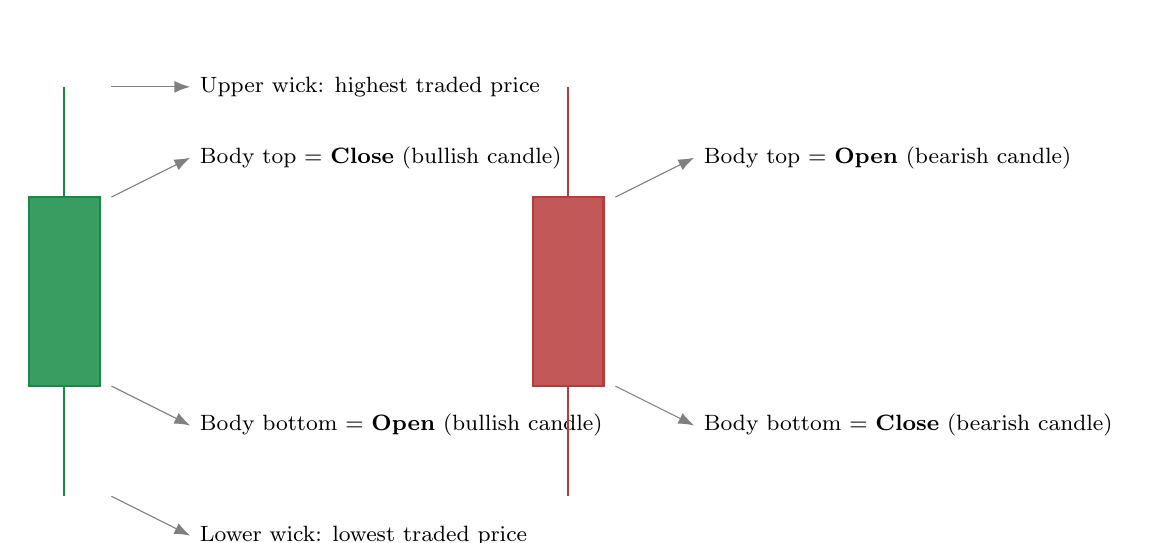
\begin{tikzpicture}[x=1.0cm,y=1.0cm]
  % Green (bullish) candle anatomy
  \draw[bullc,thick] (0,0) -- (0,5.2);
  \fill[bullc!85] (-0.45,1.4) rectangle (0.45,3.8);
  \draw[bullc,thick] (-0.45,1.4) rectangle (0.45,3.8);
  \draw[-{Latex[length=2mm]},gray] (0.6,5.2) -- (1.6,5.2) node[right,black,font=\footnotesize]{Upper wick: highest traded price};
  \draw[-{Latex[length=2mm]},gray] (0.6,3.8) -- (1.6,4.3) node[right,black,font=\footnotesize]{Body top = \textbf{Close} (bullish candle)};
  \draw[-{Latex[length=2mm]},gray] (0.6,1.4) -- (1.6,0.9) node[right,black,font=\footnotesize]{Body bottom = \textbf{Open} (bullish candle)};
  \draw[-{Latex[length=2mm]},gray] (0.6,0) -- (1.6,-0.5) node[right,black,font=\footnotesize]{Lower wick: lowest traded price};
  % Red (bearish) candle anatomy, shown alongside
  \begin{scope}[xshift=6.4cm]
    \draw[bearc,thick] (0,0) -- (0,5.2);
    \fill[bearc!85] (-0.45,1.4) rectangle (0.45,3.8);
    \draw[bearc,thick] (-0.45,1.4) rectangle (0.45,3.8);
    \draw[-{Latex[length=2mm]},gray] (0.6,3.8) -- (1.6,4.3) node[right,black,font=\footnotesize]{Body top = \textbf{Open} (bearish candle)};
    \draw[-{Latex[length=2mm]},gray] (0.6,1.4) -- (1.6,0.9) node[right,black,font=\footnotesize]{Body bottom = \textbf{Close} (bearish candle)};
  \end{scope}
\end{tikzpicture}
\end{center}

\begin{itemize}[leftmargin=*]
    \item \textbf{Open:} The price at the beginning of the period.
    \item \textbf{Close:} The price at the end of the period.
    \item \textbf{High:} The absolute highest price reached during the period.
    \item \textbf{Low:} The absolute lowest price reached during the period.
\end{itemize}

\paragraph{Anatomy of a Candlestick}
\begin{itemize}[leftmargin=*]
    \item \textbf{The Body:} The thick, shaded or colored portion represents the range between the open and close prices.
    \item \textbf{Green/White Body:} Indicates bullish sentiment; the closing price was higher than the opening price. The lower end is the open, and the upper end is the close.
    \item \textbf{Red/Black Body:} Indicates bearish sentiment; the closing price was lower than the opening price. The upper end is the open, and the lower end is the close.
    \item \textbf{The Wicks or Shadows:} The thin lines extending above and below the body show the full trading range, from high to low, during that specific time frame.
\end{itemize}

\subsubsection{Why Use Candlestick Charts?}
Candlestick charts are preferred over simple line charts because they offer a deeper, more immediate understanding of market dynamics.

\begin{itemize}[leftmargin=*]
    \item \textbf{Visual Efficiency:} They provide a quick snapshot of market sentiment, such as bullishness or bearishness, at a glance.
    \item \textbf{Predictive Value:} Specific individual candles or multi-candle patterns can signal potential trend reversals or the continuation of an existing trend.
    \item \textbf{Actionable Insights:} Traders rely on these patterns to identify precise entry and exit points for their trades.
    \item \textbf{Momentum Tracking:} Candlesticks help gauge market momentum and visualize price action better than basic charts. A candlestick chart can convey useful information such as trend, bullishness, bearishness, and volume context.
\end{itemize}

\subsubsection{Analyzing Candlestick Charts for Day Trading}

\paragraph{Time Frames}
Candlesticks represent different durations depending on the selected chart. For instance, in a 5-minute chart, one candle represents 5 minutes of trading; in a 10-minute chart, it represents 10 minutes.

\begin{itemize}[leftmargin=*]
    \item \textbf{Scalping/Day Trading:} 5-minute, 10-minute, or 15-minute charts are used to capture small price fluctuations quickly.
    \item \textbf{Larger Movements:} 30-minute, 1-hour, 3-hour, and daily charts are used to study broader price action.
\end{itemize}

\paragraph{Price Action Analysis}
Reading candlestick charts forms the basis of price action analysis, allowing traders to predict near-future movements by observing current fluctuations. The primary goal in day trading is identifying the overarching trend:

\begin{itemize}[leftmargin=*]
    \item \textbf{Uptrend:} The stock is consistently moving higher. The action bias is to look for long or buy opportunities.
    \item \textbf{Downtrend:} The stock is consistently moving lower. The action bias is to be cautious with long positions or to look for short-side opportunities where appropriate.
\end{itemize}

\paragraph{Assessing Bullish and Bearish Strength}
\begin{itemize}[leftmargin=*]
    \item \textbf{Full Body Candles:} Indicate strong buying when green or strong selling when red because the stock traded strongly through that range.
    \item \textbf{Long Wicks:} A long upper and lower wick on a single candle indicates price volatility: the price swung widely but did not sustain those levels.
    \item \textbf{Wick Positioning:} A body at the upper end with a long lower wick suggests bulls are in control. A body at the lower end with a long upper wick suggests bears are in control.
\end{itemize}

\paragraph{Trend Phases}
\begin{itemize}[leftmargin=*]
    \item \textbf{Trends and Corrections:} A stock rarely moves in a perfectly straight line. A trend often looks like a wave, with periodic moves in the opposite direction before the primary trend resumes. Shortening waves may signal trend exhaustion.
    \item \textbf{Consolidation:} A phase where price moves within a narrow, horizontal range, indicating that neither buyers nor sellers are in firm control. A breakout from consolidation can signal the start of a new trend.
\end{itemize}

\subsection{25 Essential Candlestick Patterns for Trading}
Below is a detailed breakdown of the patterns discussed, categorized by their structural meaning. The diagrams are schematic: green candles close above their open, red candles close below their open, and the surrounding trend or confirmation candle is part of the pattern context.

\subsubsection{Single Candlestick Patterns}

\paragraph{Hammer}
\candlediagram{
    \drawcandle{0}{8.0}{8.9}{3.0}{8.5}{bullc}
}
\begin{itemize}[leftmargin=*]
    \item \textbf{Visual Description:} Small real body near the top of the candle, little or no upper wick, and a long lower wick usually at least twice the body size.
    \item \textbf{How to Identify:} Found near the bottom of a downtrend. It can be red or green, though a green hammer is usually stronger.
    \item \textbf{Interpretation:} Bullish reversal warning. It suggests that the downtrend may be weakening, but confirmation from the next candle is preferred.
    \item \textbf{Psychology:} Sellers pushed the price down sharply, but buyers entered aggressively and forced the close back near the high, rejecting lower prices.
\end{itemize}

\paragraph{Hanging Man}
\candlediagram{
    \drawcandle{0}{8.5}{8.9}{3.0}{8.0}{bearc}
}
\begin{itemize}[leftmargin=*]
    \item \textbf{Visual Description:} Same shape as a hammer: small body near the top, little or no upper wick, and a long lower wick.
    \item \textbf{How to Identify:} Found near the top of an uptrend.
    \item \textbf{Interpretation:} Bearish reversal warning. It is stronger when followed by a red confirmation candle.
    \item \textbf{Psychology:} Sellers managed to push price far below the open during the session. Even if buyers recovered part of the move, the long lower wick warns that selling pressure has appeared after an advance.
\end{itemize}

\paragraph{Inverted Hammer}
\candlediagram{
    \drawcandle{0}{3.5}{9.0}{3.0}{4.0}{bullc}
}
\begin{itemize}[leftmargin=*]
    \item \textbf{Visual Description:} Small body near the bottom of the candle, little or no lower wick, and a long upper wick.
    \item \textbf{How to Identify:} Found near the bottom of a downtrend. It can be red or green.
    \item \textbf{Interpretation:} Bullish reversal warning, especially if the next candle closes higher.
    \item \textbf{Psychology:} Buyers attempted to push price upward, creating the long upper wick. Even though they could not hold the highs, sellers failed to extend the downtrend convincingly.
\end{itemize}

\paragraph{Shooting Star}
\candlediagram{
    \drawcandle{0}{4.0}{9.0}{3.1}{3.5}{bearc}
}
\begin{itemize}[leftmargin=*]
    \item \textbf{Visual Description:} Same shape as an inverted hammer: small body near the bottom and a long upper wick.
    \item \textbf{How to Identify:} Found near the top of an uptrend.
    \item \textbf{Interpretation:} Bearish reversal warning, especially if followed by a red confirmation candle.
    \item \textbf{Psychology:} Buyers pushed price higher, but sellers overwhelmed them and forced the close back near the low, rejecting higher prices.
\end{itemize}

\paragraph{Spinning Top}
\candlediagram{
    \drawcandle{0}{4.8}{8.5}{1.5}{5.2}{bullc}
}
\begin{itemize}[leftmargin=*]
    \item \textbf{Visual Description:} Small real body with long upper and lower wicks of roughly similar length.
    \item \textbf{How to Identify:} Can appear anywhere in a chart.
    \item \textbf{Interpretation:} Indecision or temporary pause. It can precede reversal or continuation depending on the next candles.
    \item \textbf{Psychology:} Both buyers and sellers moved price significantly, but neither side gained dominance, so the close remained near the open.
\end{itemize}

\paragraph{Bullish Spinning Top}
\candlediagram{
    \drawcandle{0}{7.8}{8.2}{5.2}{5.8}{bearc}
    \drawcandle{1}{5.7}{6.1}{3.2}{3.8}{bearc}
    \drawcandle{2}{4.4}{7.0}{1.8}{4.8}{bullc}
    \drawcandle{3}{5.0}{7.4}{4.6}{6.8}{bullc}
}
\begin{itemize}[leftmargin=*]
    \item \textbf{Visual Description:} A spinning top that appears after a downward move and is followed by bullish confirmation.
    \item \textbf{How to Identify:} Found near the bottom of a downtrend, preferably followed by a green candle closing above the spinning top's high.
    \item \textbf{Interpretation:} Potential bullish reversal. The spinning top shows indecision, and the confirmation candle suggests buyers are taking control.
    \item \textbf{Psychology:} Heavy selling pauses and becomes a tug-of-war. The subsequent green candle confirms that buyers have gained the upper hand.
\end{itemize}

\paragraph{Bearish Spinning Top}
\candlediagram{
    \drawcandle{0}{3.2}{5.8}{3.0}{5.4}{bullc}
    \drawcandle{1}{5.2}{7.5}{5.0}{7.1}{bullc}
    \drawcandle{2}{6.4}{9.0}{3.8}{6.0}{bearc}
    \drawcandle{3}{5.8}{6.2}{3.0}{3.6}{bearc}
}
\begin{itemize}[leftmargin=*]
    \item \textbf{Visual Description:} A spinning top that appears after an upward move and is followed by bearish confirmation.
    \item \textbf{How to Identify:} Found near the top of an uptrend, preferably followed by a red candle closing below the spinning top's low.
    \item \textbf{Interpretation:} Potential bearish reversal. The spinning top shows indecision, and the confirmation candle suggests sellers are taking control.
    \item \textbf{Psychology:} Aggressive buying stalls. The subsequent red candle confirms that sellers have taken control from exhausted buyers.
\end{itemize}

\paragraph{Doji}
\candlediagram{
    \drawdoji{0}{5.0}{8.0}{2.0}{black}
}
\begin{itemize}[leftmargin=*]
    \item \textbf{Visual Description:} Almost no real body because open and close prices are virtually identical; it often looks like a plus sign or cross.
    \item \textbf{How to Identify:} Can appear anywhere. Its color is less important than the equality between open and close.
    \item \textbf{Interpretation:} Indecision or possible reversal, especially near the extreme top or bottom of a trend.
    \item \textbf{Psychology:} Represents equilibrium between supply and demand. Neither bulls nor bears could assert dominance during the session.
\end{itemize}

\paragraph{Dragonfly Doji}
\candlediagram{
    \drawdoji{0}{8.0}{8.0}{2.0}{bullc}
}
\begin{itemize}[leftmargin=*]
    \item \textbf{Visual Description:} Looks like a T: open, close, and high are nearly equal, with a long lower wick and little or no upper wick.
    \item \textbf{How to Identify:} Most meaningful near the bottom of a downtrend.
    \item \textbf{Interpretation:} Bullish reversal warning that becomes stronger with a higher close on the next candle.
    \item \textbf{Psychology:} Sellers aggressively pushed price down, but buyers drove price back to the opening high, rejecting lower levels.
\end{itemize}

\paragraph{Gravestone Doji}
\candlediagram{
    \drawdoji{0}{2.0}{8.0}{2.0}{bearc}
}
\begin{itemize}[leftmargin=*]
    \item \textbf{Visual Description:} Looks like an inverted T: open, close, and low are nearly equal, with a long upper wick and little or no lower wick.
    \item \textbf{How to Identify:} Most meaningful near the top of an uptrend.
    \item \textbf{Interpretation:} Bearish reversal warning that becomes stronger with a lower close on the next candle.
    \item \textbf{Psychology:} Buyers pushed price sharply upward, but sellers erased the advance and forced the close back near the low, rejecting higher levels.
\end{itemize}

\paragraph{Marubozu}
\candlediagram{
    \drawcandle{0}{2.0}{8.0}{2.0}{8.0}{bullc}
    \drawcandle{1.2}{8.0}{8.0}{2.0}{2.0}{bearc}
    \node[font=\scriptsize] at (0,-0.3) {Bullish};
    \node[font=\scriptsize] at (1.2,-0.3) {Bearish};
}
\begin{itemize}[leftmargin=*]
    \item \textbf{Visual Description:} A long full-body candle with virtually no upper or lower wick.
    \item \textbf{How to Identify:} Can appear anywhere. A bullish Marubozu opens near the low and closes near the high; a bearish Marubozu opens near the high and closes near the low.
    \item \textbf{Interpretation:} Strong directional conviction. It may signal continuation or reversal depending on trend context and follow-through.
    \item \textbf{Psychology:} Shows one-sided control for nearly the entire session: buyers dominate a green Marubozu, while sellers dominate a red Marubozu.
\end{itemize}

\subsubsection{Multi-Candlestick Patterns}

\paragraph{Bullish Engulfing}
\candlediagram{
    \drawcandle{0}{5.5}{6.0}{4.0}{4.5}{bearc}
    \drawcandle{1}{4.0}{8.0}{3.7}{7.5}{bullc}
}
\begin{itemize}[leftmargin=*]
    \item \textbf{Visual Description:} A small red candle followed by a larger green candle.
    \item \textbf{How to Identify:} Found near the bottom of a downtrend. The second green real body completely engulfs the first red real body.
    \item \textbf{Interpretation:} Bullish reversal signal that is stronger when volume rises or the next candle confirms upward movement.
    \item \textbf{Psychology:} The small red candle shows sellers losing momentum, while the large green candle shows buyers aggressively overwhelming them.
\end{itemize}

\paragraph{Bearish Engulfing}
\candlediagram{
    \drawcandle{0}{4.5}{6.0}{4.0}{5.5}{bullc}
    \drawcandle{1}{7.5}{8.0}{3.7}{4.0}{bearc}
}
\begin{itemize}[leftmargin=*]
    \item \textbf{Visual Description:} A small green candle followed by a larger red candle.
    \item \textbf{How to Identify:} Found near the top of an uptrend. The second red real body completely engulfs the first green real body.
    \item \textbf{Interpretation:} Bearish reversal signal that is stronger when volume rises or the next candle confirms downward movement.
    \item \textbf{Psychology:} The small green candle shows buyers losing momentum, while the large red candle shows sellers aggressively overwhelming them.
\end{itemize}

\paragraph{Bullish Harami}
\candlediagram{
    \drawcandle{0}{8.0}{8.5}{2.5}{3.0}{bearc}
    \drawcandle{1}{4.5}{5.5}{4.2}{5.2}{bullc}
}
\begin{itemize}[leftmargin=*]
    \item \textbf{Visual Description:} A large red candle followed by a smaller green or neutral candle contained inside the previous real body.
    \item \textbf{How to Identify:} Found after a downtrend. The second candle's real body should remain within the first candle's real body.
    \item \textbf{Interpretation:} Potential bullish reversal or loss of bearish momentum, preferably confirmed by a later upward close.
    \item \textbf{Psychology:} Strong selling is followed by a much narrower session, showing that selling pressure has stalled and buyers may be entering.
\end{itemize}

\paragraph{Bearish Harami}
\candlediagram{
    \drawcandle{0}{3.0}{8.5}{2.5}{8.0}{bullc}
    \drawcandle{1}{6.0}{6.3}{5.0}{5.3}{bearc}
}
\begin{itemize}[leftmargin=*]
    \item \textbf{Visual Description:} A large green candle followed by a smaller red or neutral candle contained inside the previous real body.
    \item \textbf{How to Identify:} Found after an uptrend. The second candle's real body should remain within the first candle's real body.
    \item \textbf{Interpretation:} Potential bearish reversal or loss of bullish momentum, preferably confirmed by a later downward close.
    \item \textbf{Psychology:} Strong buying is followed by a much narrower session, showing that buying pressure has stalled and sellers may be entering.
\end{itemize}

\paragraph{Piercing Line}
\candlediagram{
    \drawcandle{0}{8.0}{8.5}{3.0}{3.5}{bearc}
    \drawcandle{1}{2.8}{6.8}{2.5}{6.4}{bullc}
    \draw[dashed,gray] (-0.35,5.75) -- (1.35,5.75);
    \node[font=\scriptsize,gray] at (1.75,5.75) {50\%};
}
\begin{itemize}[leftmargin=*]
    \item \textbf{Visual Description:} A red candle followed by a green candle that opens below the prior candle's low and closes above the midpoint of the prior red body.
    \item \textbf{How to Identify:} Found near the bottom of a downtrend. The green candle should close more than halfway into the previous red body, but usually below the previous open.
    \item \textbf{Interpretation:} Bullish reversal signal that becomes stronger with a subsequent higher close.
    \item \textbf{Psychology:} Sellers initially drive price lower, but buyers forcefully regain control and recover much of the previous session's decline.
\end{itemize}

\paragraph{Dark Cloud Cover}
\candlediagram{
    \drawcandle{0}{3.5}{8.5}{3.0}{8.0}{bullc}
    \drawcandle{1}{8.7}{9.0}{5.0}{5.2}{bearc}
    \draw[dashed,gray] (-0.35,5.75) -- (1.35,5.75);
    \node[font=\scriptsize,gray] at (1.75,5.75) {50\%};
}
\begin{itemize}[leftmargin=*]
    \item \textbf{Visual Description:} A green candle followed by a red candle that opens above the prior high and closes below the midpoint of the prior green body.
    \item \textbf{How to Identify:} Found near the top of an uptrend. The red candle should close deeply into the previous green body.
    \item \textbf{Interpretation:} Bearish reversal signal that becomes stronger with a subsequent lower close.
    \item \textbf{Psychology:} Buyers create an optimistic open, but sellers take control and erase much of the previous session's advance.
\end{itemize}

\paragraph{Morning Star}
\candlediagram{
    \drawcandle{0}{8.0}{8.5}{3.2}{3.5}{bearc}
    \drawcandle{1.2}{2.6}{3.2}{2.2}{2.9}{bullc}
    \drawcandle{2.4}{3.6}{8.5}{3.4}{8.0}{bullc}
}
\begin{itemize}[leftmargin=*]
    \item \textbf{Visual Description:} A three-candle pattern: long red candle, small-bodied candle after a downward gap or weak session, and long green candle.
    \item \textbf{How to Identify:} Found after a downtrend. The third candle should close well into the first candle's body.
    \item \textbf{Interpretation:} Bullish reversal signal indicating that buyers may have taken control.
    \item \textbf{Psychology:} Panic selling slows into indecision, then a strong green candle confirms a shift from bearish to bullish momentum.
\end{itemize}

\paragraph{Evening Star}
\candlediagram{
    \drawcandle{0}{3.5}{8.5}{3.2}{8.0}{bullc}
    \drawcandle{1.2}{8.9}{9.3}{8.4}{8.6}{bearc}
    \drawcandle{2.4}{7.8}{8.0}{3.2}{3.5}{bearc}
}
\begin{itemize}[leftmargin=*]
    \item \textbf{Visual Description:} A three-candle pattern: long green candle, small-bodied candle after an upward gap or strong session, and long red candle.
    \item \textbf{How to Identify:} Found after an uptrend. The third candle should close well into the first candle's body.
    \item \textbf{Interpretation:} Bearish reversal signal indicating that sellers may have taken control.
    \item \textbf{Psychology:} Euphoric buying slows into indecision, then a strong red candle confirms a shift from bullish to bearish momentum.
\end{itemize}

\paragraph{Bullish Abandoned Baby}
\candlediagram{
    \drawcandle{0}{8.0}{8.5}{3.8}{4.0}{bearc}
    \drawdoji{1.2}{2.5}{2.8}{2.2}{black}
    \drawcandle{2.4}{3.8}{8.2}{3.5}{7.8}{bullc}
}
\begin{itemize}[leftmargin=*]
    \item \textbf{Visual Description:} Similar to a Morning Star, but the middle candle is a Doji separated by gaps on both sides.
    \item \textbf{How to Identify:} Found after a downtrend. The Doji should be isolated below the first and third candles.
    \item \textbf{Interpretation:} Strong bullish reversal signal, especially when the third candle closes firmly upward.
    \item \textbf{Psychology:} Sellers exhaust themselves into an isolated Doji, then buyers take control with a sharp move upward.
\end{itemize}

\paragraph{Bearish Abandoned Baby}
\candlediagram{
    \drawcandle{0}{4.0}{8.2}{3.8}{8.0}{bullc}
    \drawdoji{1.2}{9.0}{9.3}{8.7}{black}
    \drawcandle{2.4}{8.2}{8.5}{3.8}{4.0}{bearc}
}
\begin{itemize}[leftmargin=*]
    \item \textbf{Visual Description:} Similar to an Evening Star, but the middle candle is a Doji separated by gaps on both sides.
    \item \textbf{How to Identify:} Found after an uptrend. The Doji should be isolated above the first and third candles.
    \item \textbf{Interpretation:} Strong bearish reversal signal, especially when the third candle closes firmly downward.
    \item \textbf{Psychology:} Buyers exhaust themselves into an isolated Doji, then sellers take control with a sharp move downward.
\end{itemize}

\paragraph{Three White Soldiers}
\candlediagram{
    \drawcandle{0}{2.5}{5.8}{2.2}{5.5}{bullc}
    \drawcandle{1}{4.8}{7.5}{4.5}{7.2}{bullc}
    \drawcandle{2}{6.5}{9.0}{6.2}{8.8}{bullc}
}
\begin{itemize}[leftmargin=*]
    \item \textbf{Visual Description:} Three consecutive long green candles, each closing higher than the previous candle.
    \item \textbf{How to Identify:} Found after a downtrend. Each candle typically opens within the previous candle's real body and closes near its high.
    \item \textbf{Interpretation:} Strong bullish reversal or continuation signal, but traders should avoid chasing if the candles are extremely extended.
    \item \textbf{Psychology:} Sustained buying pressure over three periods overwhelms remaining sellers from the prior downtrend.
\end{itemize}

\paragraph{Three Black Crows}
\candlediagram{
    \drawcandle{0}{8.8}{9.0}{5.8}{6.0}{bearc}
    \drawcandle{1}{6.8}{7.0}{4.0}{4.2}{bearc}
    \drawcandle{2}{5.0}{5.2}{2.2}{2.5}{bearc}
}
\begin{itemize}[leftmargin=*]
    \item \textbf{Visual Description:} Three consecutive long red candles, each closing lower than the previous candle.
    \item \textbf{How to Identify:} Found after an uptrend. Each candle typically opens within the previous candle's real body and closes near its low.
    \item \textbf{Interpretation:} Strong bearish reversal or continuation signal, but traders should avoid chasing if the candles are extremely extended.
    \item \textbf{Psychology:} Sustained selling pressure over three periods overwhelms remaining buyers from the prior uptrend.
\end{itemize}

\paragraph{Gap Up}
\candlediagram{
    \drawcandle{0}{3.0}{5.0}{2.0}{4.2}{bullc}
    \drawcandle{1.2}{6.2}{8.5}{6.0}{8.0}{bullc}
    \draw[<->,gray] (0.6,5.05) -- (0.6,5.95);
    \node[font=\scriptsize,gray] at (1.15,5.5) {gap};
}
\begin{itemize}[leftmargin=*]
    \item \textbf{Visual Description:} A new candle opens and trades above the previous candle's high, leaving visible empty space on the chart.
    \item \textbf{How to Identify:} The second candle's low is above the first candle's high.
    \item \textbf{Interpretation:} Strong bullish sentiment or positive repricing; follow-through depends on volume and whether the gap holds.
    \item \textbf{Psychology:} Buyers are eager enough to pay significantly higher prices immediately, bypassing lower levels.
\end{itemize}

\paragraph{Gap Down}
\candlediagram{
    \drawcandle{0}{7.2}{8.5}{6.0}{6.3}{bearc}
    \drawcandle{1.2}{4.0}{5.0}{2.0}{3.0}{bearc}
    \draw[<->,gray] (0.6,5.05) -- (0.6,5.95);
    \node[font=\scriptsize,gray] at (1.15,5.5) {gap};
}
\begin{itemize}[leftmargin=*]
    \item \textbf{Visual Description:} A new candle opens and trades below the previous candle's low, leaving visible empty space on the chart.
    \item \textbf{How to Identify:} The second candle's high is below the first candle's low.
    \item \textbf{Interpretation:} Strong bearish sentiment or sudden negative repricing. Follow-through depends on volume and whether the gap holds.
    \item \textbf{Psychology:} Sellers are urgent enough to accept significantly lower prices immediately, bypassing higher levels.
\end{itemize}

\subsubsection{Expert Trading Advice}
While patterns are powerful, they should not be traded blindly.

\begin{itemize}[leftmargin=*]
    \item \textbf{Wait for Confirmation:} Do not take action based on a single pattern formation. Wait for subsequent candles to confirm the anticipated direction.
    \item \textbf{Consider Macro Context:} Market conditions and breaking news, such as border tensions, regulatory changes, or dividend announcements, can cause sudden shifts that override technical chart patterns.
    \item \textbf{Use Confluence:} Successful traders combine candlestick patterns with other technical indicators and comprehensive trading strategies to increase their probability of success.
\end{itemize}


\subsection{Volume in the Stock Market}
\index{Volume}
\index{Relative Volume}
\index{On-Balance Volume}
\index{Chaikin Money Flow}
\index{Klinger Oscillator}

\subsubsection{What is Trading Volume?}
In stock trading, \textbf{volume} represents the total number of financial assets, such as shares or contracts, that change hands during a specific timeframe. It is a critical indicator of market activity, liquidity, and sentiment.

\begin{itemize}[leftmargin=*]
    \item \textbf{Stocks:} Measured by the number of shares traded.
    \item \textbf{Futures \& Options:} Measured by the number of contracts traded.
\end{itemize}

\paragraph{Why Volume Matters}
\begin{itemize}[leftmargin=*]
    \item \textbf{High Volume:} Indicates high liquidity and strong market interest. It allows traders to enter and exit large positions more easily without significantly affecting the asset's price.
    \item \textbf{Low Volume:} Suggests limited interest and low liquidity, making it difficult to execute large trades without causing erratic price shifts.
    \item \textbf{Timing:} Volume typically peaks during the opening and closing periods of a trading session.
\end{itemize}

\subsubsection{Relative Volume (RVOL)}
While raw volume provides the total number of trades, \textbf{Relative Volume (RVOL)} determines whether that level of activity is normal or unusually high for a specific asset.

RVOL is a ratio that compares current activity to historical averages:

\begin{equation*}
    RVOL = \frac{\text{Current Volume}}{\text{Average Historical Volume}}
\end{equation*}

\begin{quote}
\textit{Example: If a stock's historical average is 500,000 shares per day, but it has traded 1,000,000 shares today, the RVOL is 2, meaning it is trading at twice its normal activity.}
\end{quote}

\paragraph{The Importance of RVOL}
\begin{itemize}[leftmargin=*]
    \item \textbf{Highlights Unusual Activity:} High RVOL is often a direct reaction to earnings reports, breaking news, or macroeconomic triggers.
    \item \textbf{Confirms Price Moves:} Breakouts or price trends accompanied by high RVOL are significantly more reliable and more likely to sustain.
    \item \textbf{Indicates Liquidity:} A high RVOL generally implies better liquidity during that specific trading session.
\end{itemize}

\subsubsection{The Relationship Between Price and Volume}
Traders continuously analyze volume alongside price action to gauge the true strength of a market move. Volume acts as an important confirmation tool.

\begin{itemize}[leftmargin=*]
    \item \textbf{Rising price with increasing volume:} Bullish momentum; the upward trend is backed by genuine buying conviction.
    \item \textbf{Falling price with decreasing volume:} Downward trend with waning participation.
    \item \textbf{Price and volume moving in opposite directions:} Uncertainty or potential reversal; the current trend lacks conviction, so a major change in trend direction becomes more probable.
\end{itemize}

\begin{quote}
\textit{Note: High volume does not inherently mean a stock's price will rise; heavy volume on a red candle signifies immense selling pressure.}
\end{quote}

\subsubsection{Key Volume Indicators}
Volume indicators apply mathematical formulas to raw volume data, producing visual overlays that help traders confirm trends, spot divergences, and identify entry/exit points.

\paragraph{On-Balance Volume (OBV)}
Created by Joseph Granville in 1963, OBV is a cumulative indicator that measures buying and selling pressure to reflect crowd sentiment.

\begin{itemize}[leftmargin=*]
    \item If the current closing price is \textbf{greater} than the previous close:
    \begin{equation*}
        OBV_{\text{current}} = OBV_{\text{previous}} + \text{Volume}_{\text{current}}
    \end{equation*}

    \item If the current closing price is \textbf{less} than the previous close:
    \begin{equation*}
        OBV_{\text{current}} = OBV_{\text{previous}} - \text{Volume}_{\text{current}}
    \end{equation*}

    \item If the current closing price is \textbf{equal} to the previous close:
    \begin{equation*}
        OBV_{\text{current}} = OBV_{\text{previous}}
    \end{equation*}
\end{itemize}

\paragraph{Chaikin Money Flow (CMF)}
Developed by Marc Chaikin in the 1980s, CMF identifies short-term money-flow divergence. It uses a standard 21-day period to measure the volume-weighted average of buying and selling. Values oscillate between $+1$, indicating strong buying, and $-1$, indicating strong selling, with the zero line representing equilibrium.

\begin{enumerate}[leftmargin=*]
    \item \textbf{Step 1: Calculate the Money Flow Multiplier.}
    \begin{equation*}
        \text{Multiplier} = \frac{(\text{Close} - \text{Low}) - (\text{High} - \text{Low})}{\text{High} - \text{Low}}
    \end{equation*}

    \item \textbf{Step 2: Calculate the Money Flow Volume.}
    \begin{equation*}
        \text{MFV} = \text{Multiplier} \times \text{Volume}
    \end{equation*}

    \item \textbf{Step 3: Calculate the CMF.}
    \begin{equation*}
        CMF = \frac{\text{21-day Average of Daily MFV}}{\text{21-day Average of Volume}}
    \end{equation*}
\end{enumerate}

\paragraph{Klinger Oscillator}
Developed by Stephen Klinger in 1977, this tool measures the long-term trend of money flow while remaining highly sensitive to short-term price fluctuations. It relies heavily on Volume Force and Exponential Moving Averages (EMA).

\subsubsection{Interpreting Volume Data on Charts}
Trading volume is typically displayed at the bottom of an asset's candlestick price chart as a series of vertical bars.

\begin{itemize}[leftmargin=*]
    \item \textbf{Green Volume Bars (Buying Volume):} Indicates transactions primarily settled at the ask price, pushing the stock price upward.
    \item \textbf{Red Volume Bars (Selling Volume):} Indicates transactions primarily settled at the bid price, exerting downward pressure on the stock price.
\end{itemize}

Volume data can be adjusted to any time frame, such as hourly, daily, or weekly, and is widely accessible through broker platforms, stock exchanges, and financial news sites. Used correctly, it allows investors to distinguish between a minor price pull-back and a structural market reversal.


\section{How Do Stock Prices Change?}
\index{Stock prices}
\index{Supply and demand}
\index{Order book}
\index{Market microstructure}

\subsection{Dynamics of Stock Prices and Market Microstructure}

\subsubsection{Why Do Stock Prices Change?}
Stock prices are inherently unpredictable and fluctuate based on a complex interaction of microeconomic and macroeconomic variables. These variables fundamentally alter the supply and demand for a specific asset.

\paragraph{Supply and Demand}
\begin{itemize}[leftmargin=*]
    \item \textbf{The Core Principle:} Supply and demand form the foundational driver of all markets. If demand for a stock is high while supply is limited, the price increases. Conversely, if there is a surplus of sellers, meaning high supply, and few buyers, meaning low demand, the price decreases.
\end{itemize}

\paragraph{Company Performance: Fundamentals}
\begin{itemize}[leftmargin=*]
    \item \textbf{Positive Drivers:} Strong earnings reports, new product launches, strategic acquisitions, and business expansions can boost investor confidence and drive valuations higher.
    \item \textbf{Negative Drivers:} Poor earnings, legal lawsuits, management controversies, and operational setbacks can erode confidence and cause prices to drop.
\end{itemize}

\paragraph{Economic Factors: Macroeconomics}
\begin{itemize}[leftmargin=*]
    \item \textbf{Key Indicators:} Broader economic conditions such as interest rates, inflation, GDP growth, and employment levels influence the entire market.
    \item \textbf{Example:} Lower interest rates combined with robust economic growth typically support higher stock prices, because borrowing is cheap and investors are optimistic about future corporate expansion.
\end{itemize}

\paragraph{Industry Trends and Competition}
\begin{itemize}[leftmargin=*]
    \item \textbf{Sector Tailwinds:} Technological advancements, surging consumer demand, and favorable regulatory shifts can elevate expectations for entire industries.
    \item \textbf{Sector Headwinds:} Increased competition, structural industry disruptions, and declining demand can negatively affect investor expectations and suppress prices.
\end{itemize}

\paragraph{Investor Sentiment and Market Psychology}
\begin{itemize}[leftmargin=*]
    \item \textbf{Emotional Drivers:} Market movements are heavily influenced by human psychology, especially confidence, fear, uncertainty, speculation, and momentum trading.
    \item \textbf{Impact:} These behavioral factors frequently drive sharp short-term price fluctuations that may temporarily diverge from a company's underlying fundamentals.
\end{itemize}

\paragraph{Political and Geopolitical Events}
\begin{itemize}[leftmargin=*]
    \item \textbf{Catalysts for Volatility:} Elections, changes in government policies, tax reforms, trade agreements, and international conflicts inject uncertainty into the market and can abruptly alter investor behavior and asset pricing.
\end{itemize}

\subsection{Understanding Price Determination: The Order Book}
To understand exactly how the factors above translate into a specific market price, one must understand the exchange's matching mechanism.

\subsubsection{What is an Order Book?}
An order book, also known as a \textbf{continuous book}, is a real-time electronic ledger maintained by a financial exchange. It records and displays all outstanding buy and sell orders for a specific financial asset, such as stocks, derivatives, bonds, or currencies.

\begin{itemize}[leftmargin=*]
    \item \textbf{Structure:} It organizes \textbf{bid} orders, or buy offers, and \textbf{ask} orders, or sell offers, by price level.
    \item \textbf{Contents:} It houses various order types, including market orders, limit orders, stop-loss orders, and trailing stop-loss orders.
\end{itemize}

\subsubsection{Key Insights Provided by the Order Book}
Because the order book updates continuously throughout the trading day, observing how orders accumulate, execute, or get canceled allows traders to gauge:

\begin{itemize}[leftmargin=*]
    \item Real-time market sentiment and short-term buying or selling pressure.
    \item Market depth and order imbalances.
    \item The spread between the highest bid and the lowest ask.
    \item Participant activity, which can help distinguish between retail activity and large institutional flows.
\end{itemize}

\subsubsection{Advantages \& Trading Strategies}
\begin{enumerate}[leftmargin=*]
    \item \textbf{Identifying Support and Resistance:} By locating price levels with large concentrations of buy orders, or support, and sell orders, or resistance, traders can anticipate where a stock's price is likely to bounce or stall.
    \item \textbf{Trend Analysis \& Reversals:} Traders monitor the book to determine whether a current trend has the momentum to continue or whether order flow suggests that the market is about to reverse, helping guide precise entry and exit points.
    \item \textbf{Algorithmic \& Quantitative Trading:} Market participants who favor technical analysis over fundamental analysis rely heavily on order book data to build automated trading algorithms and seek a quantitative edge.
    \item \textbf{Transparency \& Regulation:} While some institutional entities attempt to conceal trades using dark pools, the general transparency of the order book allows regulatory bodies, such as the SEC, to monitor for market delinquencies, fraud, and manipulation.
\end{enumerate}

\subsubsection{Real-World Example: NASDAQ TotalView}
\begin{itemize}[leftmargin=*]
    \item NASDAQ TotalView is regarded as one of the most comprehensive order books in the US and globally. It provides deep data for securities listed on both the NASDAQ and NYSE, equipping traders, investors, and analysts with historical trading volumes, precise price data, and advanced tools for navigating the markets.
\end{itemize}

\subsection{Bid-Ask Spread: Study Notes}
\index{Bid-ask spread}
\index{Market microstructure!bid-ask spread}
\index{Liquidity!bid-ask spread}
\index{Market makers}
\index{Transaction costs}
\index{Effective spread}

\subsubsection{What Is the Bid-Ask Spread?}
Every tradable security has \textbf{two simultaneously quoted prices} at any moment, not one:

\begin{itemize}[leftmargin=*]
    \item \textbf{Bid Price:} The highest price a buyer, trader, investor, or market maker is currently willing to \textbf{pay} to purchase the security.
    \item \textbf{Ask Price or Offer Price:} The lowest price a seller or market maker is currently willing to \textbf{accept} to sell the security.
\end{itemize}

The \textbf{bid-ask spread} is the difference between these two prices:

\begin{equation*}
    \boxed{\text{Bid-Ask Spread} = \text{Ask Price} - \text{Bid Price}}
\end{equation*}

The spread is much more than a technical detail. It is simultaneously the principal transaction cost of trading outside explicit commissions, a real-time barometer of market liquidity, and a reflection of supply-demand dynamics, market-maker risk, and overall market structure.

\subsubsection{The Two Key Players in Every Transaction}
Understanding the spread requires identifying who stands on each side of a trade.

\begin{description}[leftmargin=*,style=nextline]
    \item[Price Taker: Trader or Investor] The party that \textbf{initiates} a trade by accepting a currently quoted price. Price takers demand immediacy: they want to buy or sell right now. To \textbf{buy}, they pay the \textbf{ask price}; to \textbf{sell}, they receive the \textbf{bid price}.
    \item[Market Maker: Counterparty] The party that \textbf{stands ready} to buy or sell at any time by continuously quoting two-sided prices, meaning both bid and ask quotes. Market makers can be brokerage-employed traders, independent proprietary trading firms, or electronic systems and algorithms.
\end{description}

Market makers provide immediacy to price takers and earn compensation through the spread. A market maker \textbf{buys} at the \textbf{bid price} from sellers and \textbf{sells} at the \textbf{ask price} to buyers.

\begin{quote}
\textit{Key insight: The spread is the market maker's compensation for providing immediacy and for assuming inventory risk.}
\end{quote}

\subsubsection{The Spread as Transaction Cost}
When a trader executes a market order, they buy at the ask and sell at the bid. Therefore, the round-trip cost of entering and exiting a position is effectively the spread. The trader starts underwater by exactly the spread amount the moment the position is entered. This is what brokerages mean when they say revenue comes from traders \textbf{crossing the spread}.

This matters even in commission-free trading. A trade may have no explicit commission, but it is not truly free if the execution cost is embedded in the bid-ask spread.

\subsubsection{Order Book Depth and How It Shapes the Spread}
The spread is not fixed. It is a dynamic result of \textbf{resting limit orders} in the order book.

\begin{itemize}[leftmargin=*]
    \item \textbf{Many bid limit orders:} Competitive buyers push the highest bid upward, creating a \textbf{narrower spread}.
    \item \textbf{Few bid limit orders:} Weak demand causes the highest bid to fall, creating a \textbf{wider spread}.
    \item \textbf{Many ask limit orders:} Competitive sellers push the lowest ask downward, creating a \textbf{narrower spread}.
    \item \textbf{Few ask limit orders:} Limited selling interest causes the lowest ask to rise, creating a \textbf{wider spread}.
\end{itemize}

\paragraph{Practical implication:} When placing a buy-limit order, always check the current spread. If the limit price sits inside the spread but no counterparty is willing to meet it, the order will remain unfilled.

\subsubsection{Spread Calculations: From Basic to Advanced}
The most basic formula is:

\begin{equation*}
    \text{Spread} = \text{Ask} - \text{Bid}
\end{equation*}

For example, if the bid is \$19 and the ask is \$20, then the spread is \$1.00.

\paragraph{Percentage Spread}
The percentage spread converts the dollar spread into a relative metric that is useful for comparing securities with different price levels:

\begin{equation*}
    \text{Percentage Spread} = \frac{\text{Ask} - \text{Bid}}{\text{Ask}} \times 100\%
\end{equation*}

For example, if the spread is \$1 and the ask is \$20, then the percentage spread is $5\%$. This makes the cost meaningful in context: a \$1 spread on a \$20 stock is far more significant than the same \$1 spread on a \$500 stock, where it is only $0.2\%$.

\begin{quote}
\textit{Note: Some formulations use the midpoint or the current stock price as the denominator instead of the ask. The key is to use a consistent base for comparison.}
\end{quote}

\paragraph{Midpoint}
The midpoint is the theoretical fair price between buyers and sellers:

\begin{equation*}
    \text{Midpoint} = \frac{\text{Bid} + \text{Ask}}{2}
\end{equation*}

It is a key reference point for calculating the effective spread and assessing price improvement.

\paragraph{Effective Spread}
The \textbf{effective spread} measures the actual cost of a completed market order. It accounts for the possibility that an order may receive \textbf{price improvement}, meaning it fills better than the quoted price, or may \textbf{walk the book}, meaning it fills worse than the top quote because the order consumes multiple price levels.

For a buy order:

\begin{align*}
    \text{Effective Half-Spread} &= \text{Execution Price} - \text{Midpoint}, \\
    \text{Effective Spread} &= 2 \times (\text{Execution Price} - \text{Midpoint}).
\end{align*}

For a sell order:

\begin{equation*}
    \text{Effective Spread} = 2 \times (\text{Midpoint} - \text{Execution Price}).
\end{equation*}

For example, if the midpoint is \$20.00 and a market buy fills at \$20.05, then the effective half-spread is \$0.05 and the effective round-trip spread is \$0.10. The effective spread is a more accurate measure of true trading cost than the quoted spread, especially in highly liquid markets where quote-to-fill differences are common.

\paragraph{Weighted Average Spread}
In a layered order book with multiple price levels, the quoted best bid and best ask only show the top of the book. Larger orders can consume multiple levels, making the true execution cost higher. A \textbf{weighted average spread} accounts for this by:

\begin{enumerate}[leftmargin=*]
    \item Weighting each price tier by the volume available at that level.
    \item Computing a volume-weighted average ask and a volume-weighted average bid.
    \item Defining the weighted spread as the weighted average ask minus the weighted average bid.
\end{enumerate}

This is especially important for institutional traders executing large block orders, because the simple quoted spread may dramatically understate execution cost.

\subsubsection{The Spread as a Liquidity Measure}
\textbf{Market liquidity} is the ease with which an asset can be bought or sold without materially moving its price. The bid-ask spread is one of the most direct real-time measures of liquidity:

\begin{align*}
    \text{Narrow spread} &\Rightarrow \text{High liquidity}, \\
    \text{Wide spread} &\Rightarrow \text{Low liquidity}.
\end{align*}

\paragraph{Supply and Demand of Liquidity}
Price takers \textbf{demand liquidity} because they want immediate execution. Market makers \textbf{supply liquidity} by posting prices at which immediate trades can occur. The spread is therefore the \textbf{price of immediacy}.

Typical spread behavior varies across markets:

\begin{itemize}[leftmargin=*]
    \item \textbf{Major FX pairs, such as EUR/USD:} Very narrow spreads, often around $0.01\%$ or fractions of a penny.
    \item \textbf{Large-cap US stocks, such as AAPL or MSFT:} Spreads are often just pennies, commonly around \$0.01.
    \item \textbf{Small-cap stocks:} Spreads can reach $1$--$2\%$ of the ask price or more.
    \item \textbf{Exotic derivatives and options:} Spreads can be very wide relative to the instrument's price.
\end{itemize}

\paragraph{Perceived Risk and Inventory Risk}
Spreads also reflect \textbf{market-maker risk}. Wider spreads are demanded when:

\begin{itemize}[leftmargin=*]
    \item The security's price can move rapidly and unpredictably, meaning volatility is high.
    \item The market maker faces \textbf{adverse selection}, or the risk of trading against a counterparty with superior information.
    \item Hedging costs are high, as with complex derivatives.
\end{itemize}

Options and futures often show spreads that are a much larger percentage of their price than equities or FX because of these risk and hedging considerations.

\subsubsection{Factors That Determine Spread Width}
Seven key factors shape the spread at any moment, and they are deeply interrelated:

\begin{enumerate}[leftmargin=*]
    \item \textbf{Market Liquidity:} More buyers and sellers create more competition and a tighter spread. Fewer participants create wider spreads.
    \item \textbf{Volatility:} Higher price uncertainty causes market makers to widen spreads to protect against adverse price moves between quote and execution. Earnings announcements, geopolitical events, and major macroeconomic releases often cause temporary spread widening.
    \item \textbf{Trading Volume:} Higher volume typically narrows spreads through increased efficiency. However, a volume spike in an inherently illiquid stock may not narrow the spread if the underlying order-book depth remains thin.
    \item \textbf{Asset Class:} Large-cap equities usually have narrow spreads; small-cap equities are wider; major FX pairs are among the tightest globally; exotic currencies and OTC derivatives can be wide; options and futures can be wide relative to price.
    \item \textbf{Time of Day:} Market open and close often have high activity and relatively tight spreads, while midday lulls can widen spreads. In FX, the London/New York overlap is often the most liquid window. Major announcements, such as central-bank decisions, can widen spreads sharply around the release before normalization.
    \item \textbf{Market Structure and Competition:} Electronic limit order books with many participants create intense competition and tight spreads. OTC markets with fewer participants, lower transparency, and higher search costs tend to have wider spreads.
    \item \textbf{Market-Maker Risk Perception:} If a market maker perceives elevated risk in a specific security, such as a rumored takeover, upcoming FDA ruling, or earnings uncertainty, they may widen the spread as self-protection.
\end{enumerate}

\subsubsection{The Role of Market Makers}
Market makers are the structural backbone of the bid-ask spread. Their key functions are:

\begin{enumerate}[leftmargin=*]
    \item \textbf{Providing Liquidity:} They continuously quote two-sided prices so buyers and sellers can find a counterparty without waiting for a natural match.
    \item \textbf{Narrowing Spreads Through Competition:} Multiple market makers compete for order flow by offering the highest bid and lowest ask, compressing spreads for all participants.
    \item \textbf{Managing Risk and Inventory:} Each trade leaves the market maker with a long or short inventory position. The spread compensates them for this risk. If they are overly long, they may lower both bid and ask to discourage additional buys and attract sellers. If they are overly short, they may raise both bid and ask to discourage sells and attract buyers.
    \item \textbf{Adapting to Market Conditions:} During high volatility or low liquidity, market makers widen spreads to account for higher adverse price risk. They continuously recalibrate quotes based on order flow, news, and price action.
    \item \textbf{Enhancing Market Efficiency:} By posting competitive prices, market makers help align executed prices with fair value and make prices more informative.
    \item \textbf{Supporting Orderly Order Flow:} Market makers absorb imbalances between buy and sell orders, preventing sudden price spikes from one-sided order pressure and smoothing price discovery.
\end{enumerate}

\subsubsection{Market Orders vs. Limit Orders: Practical Implications}
Order choice determines whether a trader pays or avoids the spread:

\begin{itemize}[leftmargin=*]
    \item \textbf{Market Order:} A buy market order pays the ask, and a sell market order receives the bid. The trader acts as a \textbf{liquidity taker} and effectively pays the full spread.
    \item \textbf{Limit Order:} The trader specifies the execution price. If the order fills at that price, the trader acts as a \textbf{liquidity provider} and may avoid paying the spread, though execution is not guaranteed.
\end{itemize}

\begin{quote}
\textit{Practical rule: When the spread is wide or shifting rapidly, avoid market orders when possible. Use limit orders to specify the exact price and reduce the risk of an unfavorable fill.}
\end{quote}

The round-trip cost with a market order equals buying at the ask and selling at the bid, so the implicit cost equals the full spread per unit.

\subsubsection{Bid-Ask Spread and Arbitrage}
\paragraph{Cross-Market Arbitrage}
Arbitrageurs exploit price discrepancies across venues. For example, if Exchange A quotes stock XYZ with a bid of \$100 while Exchange B quotes the same stock with an ask of \$99, an arbitrageur can simultaneously buy at \$99 on Exchange B and sell at \$100 on Exchange A, earning \$1 per share before costs. Such opportunities usually disappear in milliseconds once discovered.

\paragraph{Market-Making as Arbitrage}
Some algorithmic traders act as informal market makers by posting both bid and ask quotes to capture the spread itself. This is effectively arbitrage between the bid and the ask within a single market, though traders must manage net inventory risk through dynamic quote adjustment.

\paragraph{Technology Dependency}
Spread-based arbitrage is highly technology-driven. Important requirements include co-location, meaning servers placed physically near exchange matching engines; ultra-low-latency data feeds; and execution algorithms that can react in microseconds. Once an opportunity is discovered and acted upon, it disappears as other participants respond.

\subsubsection{Worked Examples}
\paragraph{Example 1: Basic Spread}
For stock XYZ, suppose the bid is \$19.00 and the ask is \$20.00. The spread is \$1.00, and the percentage spread is:

\begin{equation*}
    \frac{\$1}{\$20} \times 100\% = 5\%.
\end{equation*}

The spread narrows if a buyer raises the bid to \$19.50 or a seller lowers the ask to \$19.80.

\paragraph{Example 2: Large Trade Cost}
Suppose Apple stock has a bid of \$50.00 and an ask of \$50.05. The spread is only \$0.05, which appears trivial. However, if a trader buys 100 shares at market, they pay \$50.05 per share. The immediate theoretical sale value is \$50.00 per share, so the implicit spread cost is:

\begin{equation*}
    100 \times \$0.05 = \$5.00.
\end{equation*}

At institutional scale, a 10,000-share trade creates an implicit cost of \$500 from the spread alone. This illustrates why even tiny spreads matter at scale and why large traders focus heavily on execution quality.


\section{Stock Market Index}
\index{Stock market index}
\index{Nifty 50}
\index{Sensex}
\index{Market capitalization weighting}
\index{Free-float market capitalization}
\index{Index divisor}

\subsection{Stock Market Indices}

\subsubsection{What is a Stock Market Index?}
Tracking the individual performance of every listed company to determine the overall market direction is practically difficult because major exchanges contain thousands of listed securities. A \textbf{stock market index} solves this problem by grouping a specific selection of companies into a representative basket.

By observing a single index value, investors can quickly gauge the broad direction, sentiment, and risk appetite of a market segment. An index therefore acts like a market thermometer: it does not show every individual company's movement, but it gives a reliable summary of the selected market universe.

\subsubsection{Major Indian Broad-Market Indices}
The two primary indices that serve as bellwethers for the Indian stock market are:

\begin{itemize}[leftmargin=*]
    \item \textbf{Nifty 50:} Managed by the National Stock Exchange ecosystem through NSE Indices. It comprises 50 large-cap companies and is often remembered using the phrase \emph{Nifty Fifty}.
    \item \textbf{BSE Sensex:} Managed by BSE Limited. ``Sensex'' is short for \emph{Sensitivity Index}. It comprises 30 large-cap companies.
\end{itemize}

\paragraph{Correlation Between Nifty and Sensex}
Nifty and Sensex generally move in similar directions because both are broad-market large-cap indices and many of their constituent companies overlap. It is therefore uncommon for one to be sharply positive while the other is sharply negative, unless the difference is driven by index-specific weights or constituent-specific news.

\subsubsection{Categories of Indices}
Indices are categorized based on the segment of the market they are designed to track.

\begin{enumerate}[leftmargin=*]
    \item \textbf{Market-Capitalization Indices:} These track companies based on size.
    \begin{itemize}[leftmargin=*]
        \item \textbf{Large-Cap:} Nifty 50 and Sensex.
        \item \textbf{Mid-Cap:} Nifty Midcap indices.
        \item \textbf{Small-Cap:} Nifty Smallcap indices.
    \end{itemize}

    \item \textbf{Sector-Specific Indices:} These track companies within a particular industry or economic sector.
    \begin{itemize}[leftmargin=*]
        \item \textbf{Bank Nifty:} Comprises major banking stocks.
        \item \textbf{Fin Nifty:} Comprises financial services companies, including banks and other financial institutions.
    \end{itemize}

    \item \textbf{Strategy or Factor Indices:} These track companies based on rules such as low volatility, quality, momentum, dividend yield, or value characteristics.

    \item \textbf{Thematic Indices:} These track a market theme, such as consumption, infrastructure, technology, or energy transition.
\end{enumerate}

\subsubsection{The Core Uses of an Index}
Indices serve several important functions for market participants.

\paragraph{Benchmarking: Performance Evaluation}
An index provides a standard benchmark against which an investor can measure portfolio performance.

\begin{itemize}[leftmargin=*]
    \item \textbf{Example:} If a portfolio generates a 20\% return in a year, that may appear successful. However, if the Nifty 50 generated a 30\% return over the same period, the portfolio underperformed the broader large-cap market.
    \item \textbf{Application:} The benchmark should match the portfolio universe. A large-cap portfolio should be compared with Nifty 50 or Sensex, while a small-cap portfolio should be compared with a relevant small-cap index.
\end{itemize}

\paragraph{Trading and Derivatives}
The base index itself, often called the \textbf{spot index}, is only a calculated number and cannot be directly bought or sold like a stock. However, traders actively trade index-linked instruments in the derivatives market.

\begin{itemize}[leftmargin=*]
    \item Traders buy and sell \textbf{Futures and Options (F\&O)} contracts based on indices such as Nifty, Bank Nifty, and Fin Nifty.
    \item Unlike the spot index, derivative contracts have active buyers, sellers, bids, asks, expiries, and tradable prices on broker terminals.
\end{itemize}

\paragraph{Market Sentiment and Economic Signalling}
Indices summarize whether a market segment is broadly risk-on or risk-off. A rising broad-market index usually indicates positive sentiment, while a falling index indicates caution, pessimism, or selling pressure.

\paragraph{Passive Investing}
Index funds and exchange traded funds (ETFs) replicate indices so investors can gain diversified exposure without selecting individual stocks. This is one reason index construction methodology matters: it determines what passive investors ultimately own.

\subsection{Index Construction Methodology}
Indices are not usually simple averages where every company has equal importance. Most major equity indices use a \textbf{market-capitalization weighted methodology}, often specifically a \textbf{free-float market-capitalization weighted methodology}. This means larger companies receive higher weights and therefore have greater influence on index movement.

\subsubsection{Market Capitalization: The Starting Point}
A company's market capitalization is its total equity value in the stock market:

\begin{equation*}
    \text{Market Capitalization} = \text{Share Price} \times \text{Total Shares Outstanding}.
\end{equation*}

For example, if a company has 100 crore shares outstanding and each share trades at Rs. 200, its market capitalization is:

\begin{equation*}
    100 \text{ crore} \times 200 = \text{Rs. }20{,}000 \text{ crore}.
\end{equation*}

A market-cap weighted index gives more weight to companies with larger market capitalizations because these companies represent a larger share of the total investable equity market.

\subsubsection{Free-Float Market Capitalization}
Many modern indices use \textbf{free-float market capitalization} rather than total market capitalization. Free float refers to the shares that are actually available for public trading. Shares held by promoters, governments, strategic investors, or locked-in shareholders are often excluded because they do not freely trade in the market.

\begin{equation*}
    \text{Free-Float Market Cap} = \text{Share Price} \times \text{Free-Float Shares}.
\end{equation*}

Equivalently:

\begin{equation*}
    \text{Free-Float Market Cap} = \text{Total Market Cap} \times \text{Free-Float Factor}.
\end{equation*}

\paragraph{Why Free Float Matters}
Free-float weighting is considered more practical because it reflects the portion of a company that investors can realistically buy and sell. A company may be very large on paper, but if most of its shares are locked with promoters, only a smaller portion is actually available to the market. Free-float adjustment prevents such companies from receiving an unrealistically high index weight.

\subsubsection{How Index Weights Are Calculated}
The weight of company $i$ in a market-cap weighted index is calculated as:

\begin{equation*}
    w_i = \frac{\text{Free-Float Market Cap}_i}{\sum_{j=1}^{N} \text{Free-Float Market Cap}_j}.
\end{equation*}

Here, $N$ is the number of companies in the index, and $w_i$ is the percentage influence of company $i$ on the index.

\paragraph{Simple Example}
Suppose an index has only three companies:

\begin{center}
\begin{tabular}{|l|r|r|}
\hline
\textbf{Company} & \textbf{Free-Float Market Cap} & \textbf{Index Weight} \\
\hline
Company A & Rs. 50,000 crore & 50\% \\
\hline
Company B & Rs. 30,000 crore & 30\% \\
\hline
Company C & Rs. 20,000 crore & 20\% \\
\hline
\end{tabular}
\end{center}

The total free-float market capitalization is Rs. 1,00,000 crore. Company A receives the highest weight because it represents half of the investable value of the index universe. If Company A rises by 2\% while the other two companies are unchanged, the index rises by approximately:

\begin{equation*}
    50\% \times 2\% = 1\%.
\end{equation*}

This demonstrates why large-weight constituents can move the whole index even when many smaller constituents do not move much.

\subsubsection{How the Index Level Is Maintained: The Divisor}
An index value is typically calculated using a base value and an \textbf{index divisor}. A simplified representation is:

\begin{equation*}
    \text{Index Level} = \frac{\sum \text{Free-Float Market Capitalization of Constituents}}{\text{Index Divisor}}.
\end{equation*}

The divisor is adjusted for corporate actions such as stock splits, bonus issues, rights issues, mergers, spin-offs, and constituent changes. This prevents purely mechanical events from creating artificial jumps or drops in the index.

\paragraph{Example of Divisor Logic}
If a company undergoes a stock split, its share price falls but its number of shares increases proportionally. The company's economic value has not changed. The divisor mechanism ensures that the index does not fall simply because the stock split changed the quoted share price.

\subsubsection{Why Market-Cap Weighting Is Considered Useful}
Market-cap weighting is widely used because it has several practical advantages:

\begin{enumerate}[leftmargin=*]
    \item \textbf{Represents Economic Size:} Larger companies account for a greater share of the market's total value, so giving them larger weights reflects their economic importance.
    \item \textbf{Investability:} Free-float weighting focuses on shares available for public trading, making the index easier for funds and ETFs to replicate.
    \item \textbf{Low Turnover:} Weights adjust naturally as stock prices move, so the index does not need constant rebalancing after every price change.
    \item \textbf{Liquidity Alignment:} Larger companies usually trade more actively, so higher index weights often correspond to securities that can absorb larger investment flows.
    \item \textbf{Passive Replication:} Index funds can mirror the index by buying stocks in the same weights, which makes the methodology transparent and scalable.
\end{enumerate}

\subsubsection{Limitations of Market-Cap Weighting}
Despite its advantages, market-cap weighting has important limitations:

\begin{itemize}[leftmargin=*]
    \item \textbf{Concentration Risk:} A few mega-cap stocks can dominate the index, making the index less diversified than it appears.
    \item \textbf{Momentum Bias:} Stocks that have already risen significantly become larger weights, while stocks that have fallen become smaller weights. This can cause the index to overweight expensive stocks and underweight cheaper stocks.
    \item \textbf{Sector Imbalance:} If one sector becomes very large, the index may become heavily exposed to that sector.
    \item \textbf{Not Equal Representation:} A 50-stock index does not mean each stock contributes equally. A large constituent may matter far more than several smaller constituents combined.
\end{itemize}

\subsubsection{Rebalancing and Reconstitution}
Index providers periodically review indices to ensure they remain representative of the intended market segment.

\begin{itemize}[leftmargin=*]
    \item \textbf{Rebalancing:} Adjusting constituent weights to reflect updated free-float market capitalizations, free-float factors, and methodology rules.
    \item \textbf{Reconstitution:} Adding or removing companies based on eligibility criteria such as market capitalization, liquidity, listing history, and sector representation.
\end{itemize}

Rebalancing matters because index funds and ETFs tracking the index must adjust their portfolios accordingly. This can create temporary buying or selling pressure in stocks that are added, removed, or significantly reweighted.

\subsubsection{Equal-Weighted vs. Market-Cap Weighted Indices}
An \textbf{equal-weighted index} assigns the same weight to every constituent, while a market-cap weighted index assigns weights based on company size.

\begin{itemize}[leftmargin=*]
    \item \textbf{Equal-Weighted Index:} Gives every stock the same influence, improving diversification but requiring more frequent rebalancing.
    \item \textbf{Market-Cap Weighted Index:} Gives larger companies more influence, improving investability and reducing turnover but increasing concentration risk.
\end{itemize}

\paragraph{Key Takeaway}
A stock market index is not just a list of companies. It is a rules-based measurement system. The weighting methodology determines how much each company affects the index, how passive funds allocate capital, and how accurately the index reflects the market segment it is designed to represent.

\section{Fundamental Analysis}

\subsection{What is Fundamental Analysis?}

Fundamental Analysis (FA) evaluates a security's intrinsic value by examining the factors that drive its underlying business and industry, rather than short-term price action. The goal is to judge whether a stock is undervalued or overvalued relative to its fundamentals, so an investor can decide what to buy.

FA has two components: Quantitative Analysis (balance sheets, P\&L, cash flows --- numbers-driven) and Qualitative Analysis (business model, management quality, competitive position --- judgment-driven). Both matter; numbers tell you what happened, qualitative factors help explain why and whether it will continue.

A useful framing: anyone whose daily decisions affect a company's revenue or costs --- engineers improving efficiency, salespeople closing deals, doctors running a hospital department --- is effectively already shaping the company's financial health, even without a finance title. An accountant, by contrast, only records transactions; they don't drive the operational outcomes that determine performance. This matters because it reframes FA as understanding \emph{business} drivers, not just accounting mechanics.

\subsection{1. Macro \& Industry Analysis}

This is the outermost layer --- the environment a company operates in, which sets the ceiling and floor on what's achievable regardless of company quality.

\paragraph{Economic conditions} GDP growth (overall demand in the economy), interest rates (cost of borrowing for both the company and its customers; also affects valuation multiples), inflation (affects input costs and pricing power), and fiscal/monetary policy (government spending, taxation, central bank actions). A great company in a contracting economy still faces headwinds; a mediocre company in a booming sector can coast on tailwinds.

\paragraph{Industry trends} supply-demand dynamics (is the industry growing or saturated?), regulatory changes (can create or destroy entire business models overnight), technological disruption (risk of obsolescence), and competitive intensity (how many players are fighting for the same customers, and how that affects pricing power and margins). A company's industry largely caps its long-term growth and margin potential before you even look at the company itself.

\subsection{2. Company Analysis}

\paragraph{Business model \& competitive advantage (moat)} how does the company actually make money, what stops a competitor from copying it, and is that protection durable? Common moats:

\begin{itemize}[leftmargin=*]
    \item \emph{Brand recognition} --- allows premium pricing (e.g., consumer goods, luxury).
    \item \emph{Patents/IP} --- legal exclusivity, common in pharma and tech.
    \item \emph{Network effects} --- the product gets more valuable as more people use it (e.g., marketplaces, social platforms), making it self-reinforcing.
    \item \emph{Cost leadership} --- structurally lower costs than competitors, allowing the company to win on price while still being profitable.
\end{itemize}

The key analytical question isn't just "does an advantage exist" but "how sustainable is it" --- moats erode with technology shifts, regulation, or new entrants, so this needs periodic reassessment, not a one-time check.

\paragraph{Management \& governance} judged via leadership's track record (have past promises been delivered?), capital allocation history (do they reinvest wisely, overpay for acquisitions, or return cash sensibly?), and governance practices (board independence, related-party transactions, alignment of management incentives with shareholders). Poor governance is a common reason fundamentally "good" businesses still destroy shareholder value --- the numbers can look fine while capital is being misallocated or minority shareholders are being short-changed.

\subsection{3. The Annual Report --- Where to Find Everything}

The annual report is the primary, authoritative source --- pull it directly from the company's investor relations page rather than relying solely on secondary data aggregators. Key sections:

\begin{itemize}[leftmargin=*]
    \item \textbf{Management Discussion \& Analysis (MD\&A):} opens with commentary on the macro economy and the specific sector, then financial highlights and segment-wise discussion. This is where management explains \emph{why} the numbers look the way they do and gives forward guidance --- useful for projecting which business segments will drive future growth.
    \item \textbf{Outlook/pipeline:} disclosure of upcoming products, capacity expansions, or strategic initiatives.
    \item \textbf{Operations detail:} plant/manufacturing information, subsidiary performance, and geographic footprint --- useful for understanding diversification and operating leverage.
    \item \textbf{Corporate Governance section:} director backgrounds, qualifications, and shareholding --- a direct check on the management quality factor above.
    \item \textbf{Directors' Report and Auditor's Report.}
    \item \textbf{Financial Statements:} issued in both \emph{standalone} (parent company only) and \emph{consolidated} (including subsidiaries) form --- for a holding company or one with major subsidiaries, consolidated figures give the truer picture of overall economic exposure.
\end{itemize}

Treat the annual report as the single source of truth; use data aggregators (Yahoo Finance, Screener, etc.) for speed and cross-company comparison, but verify anything material against the filed report.

\subsection{4. Income Statement (Profit \& Loss)}

\paragraph{Purpose} shows whether a business generated a profit or loss over a period, and where that profit went (or got eaten up). This is also the source of "top line" (revenue, literally the top line of the statement) and "bottom line" (net income, the last line).

\subsubsection{Line-by-line structure and interpretation}

\paragraph{Total Revenue} Total sales generated before any costs are deducted. Figures are often reported in thousands, so "\$47,000" thousand means \$47 billion. TTM means trailing twelve months: the most recent rolling year of data, which may not align with the fiscal year-end. \emph{Interpretation:} this is the most basic growth signal, but revenue growth alone says nothing about profitability, so it must always be read alongside the lines below it.

\paragraph{Cost of Revenue (COGS)} The direct cost of producing or delivering whatever was sold. \emph{Interpretation:} a rising COGS as a percentage of revenue, or falling gross margin, often signals pricing pressure, rising input costs, or loss of operating leverage.

\paragraph{Gross Profit and Gross Margin}
\begin{equation*}
    \text{Gross Profit} = \text{Revenue} - \text{Cost of Revenue}, \qquad
    \text{Gross Margin} = \frac{\text{Gross Profit}}{\text{Revenue}}.
\end{equation*}
\emph{Interpretation:} this is the cleanest measure of how much pricing power and production efficiency a business has before overhead is considered. Comparing gross margin across years or against peers shows whether core unit economics are improving, stable, or deteriorating.

\paragraph{SG\&A} Selling, General \& Administrative expenses include marketing, salaries, and the general cost of running the company, separate from production costs. \emph{Interpretation:} if SG\&A grows faster than revenue, the business is becoming less efficient at converting sales into overhead-adjusted profit. Data aggregators sometimes show SG\&A as a lump sum; the company's filed statements provide more detail when needed.

\paragraph{Total Operating Expenses} The sum of all operating costs, including SG\&A and any other operating categories the company reports.

\paragraph{Operating Income and Operating Margin}
\begin{align*}
    \text{Operating Income} &= \text{Gross Profit} - \text{Total Operating Expenses}, \\
    \text{Operating Margin} &= \frac{\text{Operating Income}}{\text{Revenue}}.
\end{align*}
\emph{Interpretation:} this is one of the most important profitability measures because it captures the profitability of the \emph{core business} before financing costs and taxes. Around 15\% operating margin can be a healthy rough benchmark, but industry context matters. Rising operating margin alongside rising revenue suggests efficient scaling; falling margin despite revenue growth signals that growth may be coming at the expense of profitability.

\paragraph{Interest Expense} The cost of servicing debt, such as bonds, loans, and credit lines. \emph{Interpretation:} compare this against operating income to gauge how much operating profit is consumed by debt service before reaching net income.

\paragraph{Other Income/Expense, Net} Items unrelated to core operations, such as one-off gains or losses and investment income. \emph{Interpretation:} because these are non-core and often non-recurring, large swings should be treated cautiously when projecting future earnings.

\paragraph{Income Before Tax}
\begin{equation*}
    \text{Income Before Tax} = \text{Operating Income} - \text{Interest Expense} \pm \text{Other Income/Expense}.
\end{equation*}

\paragraph{Income Tax} The tax paid on income. \emph{Interpretation:} effective tax-rate changes can distort net income trends year-to-year without reflecting any change in the underlying business, so check whether a net income jump is driven by operations or by a falling tax bill.

\paragraph{Net Income}
\begin{equation*}
    \text{Net Income} = \text{Income Before Tax} - \text{Tax}.
\end{equation*}
This is the headline profit figure used in EPS, P/E, ROE, and most other valuation work.

\subsubsection{What to check, holistically}

\begin{itemize}[leftmargin=*]
    \item Both operating income and net income should be positive --- a negative operating income means the core business itself is unprofitable, which is more serious than a net loss caused by, say, a one-off tax charge.
    \item Pull as long a history as possible (ideally 10 years, though free tools like Yahoo Finance typically cap at \textasciitilde{}4 years) to separate cyclical noise from genuine trend.
    \item The single most important pattern: \textbf{does operating income grow in step with revenue?} If yes (Google's pattern: revenue \$90B\(\to\)\$161B alongside operating income \$23B\(\to\)\$36B from 2016--2019), the business scales efficiently. If revenue rises while operating income falls or turns more negative (Uber: revenue \$3.8B\(\to\)\$14.1B in 2016--2019 while operating loss widened from -\$3B to -\$8.5B, with opex eventually exceeding total revenue), that's a structural red flag, regardless of how impressive the growth headline looks. Delta's case (2016--2019) illustrates a more nuanced pattern: absolute net income rose (\$4.3B \(\to\) \$4.7B), but this was driven partly by a \emph{lower tax bill} rather than core operational improvement --- gross and operating margins were actually higher back in 2016, showing why digging into the components matters more than just glancing at the bottom line.
\end{itemize}

\subsection{5. Cash Flow Statement}

\paragraph{Why it exists} under accrual accounting (mandatory under IFRS/GAAP), revenue is recognized when \emph{earned} and expenses when \emph{incurred} --- not when cash actually moves. This means reported net income can diverge significantly from actual cash generated (e.g., a sale recorded as revenue today might not be paid for in cash for 90 days; depreciation reduces reported profit without involving any cash outflow at all). The Cash Flow Statement strips accounting adjustments back out to show real cash movement, which is critical because a company can show accounting profit while quietly running out of cash.

\paragraph{Structure} reconciles Opening Cash to Closing Cash (both pulled from the Balance Sheet) across three sections. Positive values are inflows, negative are outflows.

\begin{enumerate}[leftmargin=*]
    \item \textbf{Operating Activities} --- cash generated/consumed by core, day-to-day revenue-generating operations.
    \item \textbf{Investing Activities} --- cash spent on, or received from selling, long-term assets and investments.
    \item \textbf{Financing Activities} --- cash raised or repaid via debt (banks/bondholders) or equity (issuing shares, paying dividends, buybacks).
\end{enumerate}

\paragraph{Direct method} operating section mirrors a cash-basis P\&L directly --- cash received from customers minus cash paid to suppliers/employees minus interest/tax paid. Intuitive to read, but harder for accountants to actually compile, so it's rarely used in practice.

\paragraph{Indirect method (the standard in practice)} 

\begin{enumerate}[leftmargin=*]
    \item Start with \textbf{Net Profit/Loss} from the Income Statement.
    \item \textbf{Add back non-cash expenses} --- depreciation, amortization, and any losses on asset sales (these reduced accounting profit but involved no actual cash leaving the business). Note: a \emph{gain} on an asset sale would be subtracted, since it inflated profit without representing operating cash.
    \item \textbf{Adjust for changes in working capital} (current assets and current liabilities, excluding cash itself):
\begin{itemize}[leftmargin=*]
    \item A \emph{rise} in current assets like receivables or inventory is \textbf{subtracted} --- money tied up in unpaid invoices or unsold stock isn't cash in hand, even though it may already be counted as revenue or have consumed cash to produce.
    \item A \emph{rise} in current liabilities like payables is \textbf{added} --- the company is holding onto cash longer by delaying payment to suppliers. A \emph{fall} in payables is subtracted (cash has gone out to settle old obligations).
\end{itemize}
\end{enumerate}

\paragraph{Interpretation of working capital changes} this is one of the most useful diagnostic sections in all of FA. A company can report rising revenue and rising net income while its operating cash flow stagnates or turns negative --- usually because receivables and inventory are ballooning faster than sales. That's often an early warning sign of either aggressive revenue recognition or genuine difficulty collecting cash from customers, well before it shows up anywhere else.

\paragraph{Worked example (Tumble, fictional dating app)} 

\begin{itemize}[leftmargin=*]
    \item Net profit: \$9.65M
    \item + Non-cash D\&A: \$850K
    \item + Loss on sale of furniture: \$5K (furniture cost \$20K, accumulated depreciation \$5K \(\to\) carrying value \$15K; sold for \$10K \(\to\) \$5K loss, a non-cash item originally charged through G\&A expense on the income statement, so it must be added back here)
    \item - Increase in receivables: \$5.2M (receivables rose from \$8.85M to \$14.05M)
    \item - Decrease in payables: \$450K (payables fell from \$14.85M to \$14.4M)
    \item \textbf{= Operating Cash Flow: \$4.855M}
\end{itemize}

\begin{itemize}[leftmargin=*]
    \item Investing: -\$910K (computer equipment purchased) + \$10K (cash proceeds from the furniture sale) = \textbf{-\$900K}
    \item Financing: +\$100K (new long-term debt raised, no repayments made) + \$50K (common stock issued) - \$1M (dividends paid) = \textbf{-\$850K}
\end{itemize}

\begin{itemize}[leftmargin=*]
    \item \textbf{Net change in cash} = \$4.855M - \$0.9M - \$0.85M = \textbf{\$3.105M}, which ties out exactly against the Balance Sheet (cash rose from \$13.895M to \$17M).
\end{itemize}

\paragraph{Why this matters as a check} if your computed net change in cash doesn't match the actual Balance Sheet cash movement, you've either missed a transaction or misclassified something --- this reconciliation is effectively a built-in error check, and is also why the three statements must always be read together rather than in isolation.

\subsection{6. Balance Sheet}

\paragraph{Purpose} a snapshot (not a period) of what a company owns (Assets) versus what it owes (Liabilities + Equity) at one specific point in time. The defining identity: \textbf{Total Assets = Total Liabilities + Shareholders' Equity} --- this must always balance, which is the origin of the name.

\subsubsection{Assets}

\begin{itemize}[leftmargin=*]
    \item \textbf{Fixed Assets} --- long-term physical assets (land, machinery, buildings) requiring substantial upfront capital and used over many years. \emph{Interpretation:} steady, planned growth here (without runaway debt funding it) usually signals genuine capacity expansion.
    \item \textbf{Current Assets} --- consumed/converted within one year, primarily \emph{inventory} (finished goods plus raw materials). \emph{Interpretation:} inventory growing much faster than sales can mean unsold stock building up --- a working-capital and demand-risk warning sign (cross-reference with the Inventory Turnover Ratio below).
    \item \textbf{Financial Assets} --- investments in other companies' stocks/bonds. \emph{Interpretation:} large financial-asset holdings unrelated to the core business can sometimes indicate cash hoarding or a conglomerate structure rather than focused capital allocation.
    \item \textbf{Intangible Assets} --- non-physical assets like patents (e.g., a pharma company's drug patent). \emph{Interpretation:} valuable when tied to genuine IP-driven moats, but can also be an accounting artifact of acquisitions (see Goodwill below) rather than organically built value.
\end{itemize}

\subsubsection{Liabilities}

\begin{itemize}[leftmargin=*]
    \item \textbf{Current Liabilities} --- obligations due within 1 year, including the portion of long-term debt due in the next 12 months.
    \item \textbf{Long-term Debt} --- due beyond 1 year. \emph{Interpretation:} the key question is whether this is "manageable" relative to equity (see Debt-to-Equity below) and whether it's funding productive growth or just plugging operating losses.
    \item \textbf{Other Liabilities} --- other long-term obligations, e.g., unpaid bills due in the future.
    \item \textbf{Net Worth/Equity} --- what the company owes its owners; effectively the residual claim shareholders have on the business. Comprises:
\begin{itemize}[leftmargin=*]
    \item \emph{Paid-up Capital} --- capital raised by issuing shares.
    \item \emph{Reserves/Retained Earnings} --- the cumulative profits the company has kept (not paid out as dividends) over its life.
\end{itemize}
\end{itemize}

\subsubsection{Detailed item walkthrough (illustrated via Tata Motors, 2017--2021)}

\paragraph{Current assets} 

\begin{itemize}[leftmargin=*]
    \item \emph{Cash \& short-term investments} --- readily convertible to cash; Tata Motors showed consistent year-on-year growth here, a positive liquidity signal.
    \item \emph{Total receivables} --- amounts owed by customers for goods/services already delivered but not yet paid for; essentially "sales that haven't turned into cash yet."
    \item \emph{Total inventory} --- unsold finished goods plus raw materials.
    \item \emph{Other current assets} --- anything else converting to cash within a year.
\end{itemize}

\paragraph{Non-current assets} 

\begin{itemize}[leftmargin=*]
    \item \emph{Net loans} --- loans the company itself has extended to others (zero for Tata Motors, since it's not a lending business).
    \item \emph{Net PP\&E (property, plant \& equipment)} --- buildings, machinery, land, equipment; for Tata Motors this rose steadily, consistent with ongoing capacity investment.
    \item \emph{Goodwill} --- arises when a company pays more than the accounting (book) value of a target in an acquisition, often reflecting brand value or expected synergies; recorded as an intangible asset. \emph{Interpretation:} large goodwill balances are worth scrutinizing --- if the acquired business later underperforms, goodwill can be written down, hitting reported profit even though no new cash changes hands at that point.
    \item \emph{Intangible assets} --- patents, trademarks, and similar IP.
    \item \emph{Long-term investments} --- holdings in stocks, bonds, real estate intended to be held for the long run.
    \item \emph{Other long-term assets} --- e.g., employee advances, prepaid expenses.
\end{itemize}

\paragraph{Liabilities} 

\begin{itemize}[leftmargin=*]
    \item \emph{Accounts payable} --- money owed to suppliers/creditors; conceptually the mirror image of receivables (Tata Motors' payables also rose steadily, generally in line with growing scale of operations).
    \item \emph{Total deposits} --- relevant only to banks/NBFCs (zero for Tata Motors); for a bank, deposits are a liability (interest is paid out on them) while loans made by the bank are assets (interest is earned on them) --- the reverse of how a normal company's balance sheet works.
    \item \emph{Total other current liabilities} --- short-term obligations due within 12 months, e.g., debt due in the near term.
    \item \emph{Long-term debt} --- Tata Motors' long-term debt rose from roughly Rs.60,000 crore (2017) to roughly Rs.93,000 crore (2021); generally, lower (or at least well-covered by equity) is preferable.
    \item \emph{Deferred income tax liability} --- arises when a company's accounting tax expense differs from what tax law actually requires it to pay currently --- a future tax obligation not yet due.
    \item \emph{Other liabilities} --- pension obligations, capital leases, deferred credits, and similar items not falling into other categories.
    \item \emph{Common stock} --- capital raised through share issuance in the primary market; what subsequently trades in the secondary market.
    \item \emph{Preferred stock} --- a separate capital-raising route from common stock; preferred holders receive fixed/priority dividends and are repaid before common shareholders in bankruptcy or merger, but typically have no voting rights (common shareholders do). Not all companies issue preferred stock --- Tata Motors, for example, has none.
    \item \emph{Other equity} --- primarily accumulated reserves/retained earnings.
\end{itemize}

\subsubsection{What to check}

\begin{itemize}[leftmargin=*]
    \item \textbf{Net worth trend:} rising steadily over 5--10 years signals the business is genuinely generating and retaining value for shareholders, rather than just reporting accounting profit that doesn't accumulate.
    \item \textbf{Debt-to-Equity:} should stay "manageable" --- investigate further if it exceeds 1, as that signals liabilities exceed the equity cushion, raising insolvency risk if earnings deteriorate.
    \item \textbf{Working capital health:} current assets (including cash) should exceed current liabilities, indicating the company can meet near-term obligations without needing to raise new financing or sell long-term assets under duress.
\end{itemize}

\subsection{7. How the Three Statements Connect}

The Income Statement shows the profit generated over a period; the Balance Sheet shows the resulting assets/liabilities/equity snapshot; the Cash Flow Statement shows how much actual cash was produced, invested, and raised. None of the three tells the full story alone --- net income can be positive while cash flow is negative (working capital drag), or a company can be raising large amounts of cash through financing while its core operations are actually loss-making.

\paragraph{Worked example --- Tim's Cars (one car sold for \$100,000)} 

\paragraph{Step 1 --- Income Statement} Revenue \$100,000 - COGS \$70,000 = Gross Profit \$30,000 - SG\&A \$25,000 = \textbf{Net Income \$5,000}.

\paragraph{Step 2 --- Cash Flow Statement (indirect method), starting from that \$5,000} 

\begin{itemize}[leftmargin=*]
    \item Add back non-cash D\&A: 20\% of the \$70,000 COGS is depreciation/amortization = \$14,000 \(\to\) running total \$19,000.
    \item Adjust working capital using the Balance Sheet: Accounts Receivable rose from \$10,000 to \$15,000 (+\$5,000, subtract --- this is recorded revenue not yet collected in cash) and Inventory rose from \$40,000 to \$45,000 (+\$5,000, subtract --- cash was spent producing stock not yet sold) \(\to\) combined -\$10,000. Accounts Payable rose from \$5,000 to \$7,000 (+\$2,000, add --- the company is holding cash longer by delaying supplier payment); the current portion of debt payments stayed flat at \$1,000 (no change).
    \item \textbf{Operating Cash Flow} = \$19,000 - \$10,000 + \$2,000 = \textbf{\$11,000}.
\end{itemize}

\paragraph{Step 3 --- Investing activities} \$9,000 spent on PP\&E (\$4,500 replacing worn-out equipment + \$4,500 on additional new equipment to support growth) \(\to\) \textbf{-\$9,000}. Note that only the \emph{incremental} \$4,500 increases the non-current PP\&E balance on the Balance Sheet (50,000 \(\to\) 54,500), since the other \$4,500 simply replaced assets at the same carrying value.

\paragraph{Step 4 --- Financing activities} \$5,000 raised by issuing stock + \$5,000 raised via new long-term debt (no repayments made) \(\to\) \textbf{+\$10,000}. This pushes long-term debt on the Balance Sheet from \$10,000 to \$15,000.

\paragraph{Step 5 --- Reconciliation} Net cash change = \$11,000 (operating) - \$9,000 (investing) + \$10,000 (financing) = \textbf{\$12,000}. Adding this to the prior year's \$10,000 cash balance gives a \textbf{closing cash balance of \$22,000}, which flows directly onto this year's Balance Sheet.

\paragraph{Step 6 --- Completing the Balance Sheet} Total Current Assets = \$82,000 (including the new \$22,000 cash balance, \$15,000 receivables, \$45,000 inventory). Total Non-current Assets = \$54,500 (PP\&E). \textbf{Total Assets = \$136,500}. Total Current Liabilities = \$8,000. Total Non-current Liabilities = \$15,000 (the long-term debt). \textbf{Total Liabilities = \$23,000}. Since Assets = Liabilities + Equity, \textbf{Owner's Equity = \$136,500 - \$23,000 = \$113,500} --- the amount shareholders would theoretically be entitled to if the business were liquidated at book value.

This single transaction shows the full loop: a sale on the Income Statement feeds into Operating Cash Flow on the Cash Flow Statement (adjusted for non-cash items and working capital), which combines with Investing and Financing activity to determine the closing cash balance, which becomes an asset on the Balance Sheet --- and the Balance Sheet's other movements (new debt, new equity, new PP\&E, changed receivables/inventory/payables) are themselves the very inputs used to build the Cash Flow Statement in the first place. Real companies have thousands of transactions running through this same loop simultaneously, but the underlying mechanics never change.

\subsection{8. Key Financial Ratios}

A ratio compares one financial-statement line against another, almost always expressed as a percentage or a multiple, and is most useful when tracked over time and benchmarked against peers (a ratio in isolation, without context, is rarely meaningful on its own). They split into five groups.

\subsubsection{A. Profitability Ratios --- how efficiently the business converts revenue, assets, equity, or capital into profit}

\begingroup
\small
\setlength{\tabcolsep}{4pt}
\begin{center}\begin{tabular}{|L{0.22\textwidth}|L{0.24\textwidth}|L{0.42\textwidth}|}
\hline
\textbf{Ratio} & \textbf{Formula} & \textbf{What it tells you} \\
\hline
Gross Profit Margin & Gross Profit / Revenue & How much profit survives after direct production costs --- reflects pricing power and production efficiency. Higher and stable/rising is generally better. \\
\hline
Operating Profit Margin & Operating Profit / Revenue & Profitability after overhead too, before financing/tax --- the cleanest read on core business efficiency. \\
\hline
Net Profit Margin & Net Profit / Revenue & The final take-home profit per dollar of sales, after everything including interest and tax. \\
\hline
Return on Assets (ROA) & Net Profit / Total Assets & How efficiently the business turns its total asset base into profit --- useful for comparing capital intensity across companies. \\
\hline
Return on Equity (ROE) & Net Profit / Total Equity & How efficiently shareholders' own capital is being used to generate profit. \emph{Caveat:} heavy debt financing shrinks the equity base and can artificially inflate ROE, so a high ROE driven mainly by leverage is riskier than one driven by genuine operating efficiency --- always check D/E alongside ROE. \\
\hline
Return on Capital Employed (ROCE) & EBIT / (Total Assets - Current Liabilities) & Strips out the leverage distortion in ROE by using \emph{all} capital (debt + equity) employed in the business rather than just equity --- a better comparison tool across companies with different capital structures. \\
\hline
\end{tabular}\end{center}
\endgroup

\paragraph{General interpretation note} when comparing a P\&L figure (a flow, over a period) against a Balance Sheet figure (a snapshot, at a point in time), it's best practice to average the opening and closing Balance Sheet numbers, so you're comparing like with like.

\subsubsection{B. Liquidity Ratios --- ability to meet short-term obligations}

\begingroup
\small
\setlength{\tabcolsep}{4pt}
\begin{center}\begin{tabular}{|L{0.22\textwidth}|L{0.24\textwidth}|L{0.42\textwidth}|}
\hline
\textbf{Ratio} & \textbf{Formula} & \textbf{What it tells you} \\
\hline
Cash Ratio & Cash / Current Liabilities & The strictest test --- can the company pay off all short-term debt using only cash on hand? A ratio above 1 indicates strong liquidity, though holding excessive cash idle isn't always optimal either. \\
\hline
Quick Ratio (Acid-Test) & (Cash + Marketable Securities + Receivables) / Current Liabilities & A more realistic near-term liquidity test --- excludes inventory and prepaid expenses, since these aren't quickly convertible to cash. \\
\hline
Current Ratio & Current Assets / Current Liabilities & The broadest liquidity measure, including inventory. Generally, a ratio comfortably above 1 indicates the company can cover near-term obligations without distress; too high a ratio, though, can also suggest inefficiently parked working capital. \\
\hline
\end{tabular}\end{center}
\endgroup

\subsubsection{C. Efficiency Ratios --- how well the business moves inventory, collects cash, and pays bills}

\textbf{Turnover Ratios} (an Income Statement line against a related Balance Sheet line):

\begingroup
\small
\setlength{\tabcolsep}{4pt}
\begin{center}\begin{tabular}{|L{0.22\textwidth}|L{0.24\textwidth}|L{0.42\textwidth}|}
\hline
\textbf{Ratio} & \textbf{Formula} & \textbf{What it tells you} \\
\hline
Inventory Turnover & COGS / Inventory & How many times inventory is sold and replenished over the period --- higher generally means efficient inventory management and strong demand; very low turnover can signal obsolete or slow-moving stock. \\
\hline
Receivables Turnover & Revenue / Accounts Receivable & How efficiently the company collects cash from customers --- higher means faster collection. \\
\hline
Asset Turnover & Revenue / Total Assets & How much revenue is generated per dollar of total assets --- a measure of asset-use efficiency, related to but distinct from ROA (which uses profit instead of revenue). \\
\hline
Payables Turnover & COGS / Accounts Payable & How quickly the company pays its own suppliers --- very high turnover may mean the company isn't taking full advantage of supplier credit terms; very low can signal cash strain. \\
\hline
\end{tabular}\end{center}
\endgroup

\textbf{Cash Conversion Cycle} --- converts the turnover ratios above into "days," giving a more intuitive operational picture:

\begingroup
\small
\setlength{\tabcolsep}{4pt}
\begin{center}\begin{tabular}{|L{0.22\textwidth}|L{0.24\textwidth}|L{0.42\textwidth}|}
\hline
\textbf{Ratio} & \textbf{Formula} & \textbf{What it tells you} \\
\hline
Days Sales of Inventory (DSI) & (Inventory / COGS) \(\times\) 365 & Average days to convert inventory into a sale. Lower is generally better --- faster inventory turnover ties up less cash. \\
\hline
Days Sales Outstanding (DSO) & (Receivables / Revenue) \(\times\) 365 & Average days to collect cash after a sale. Lower means faster cash collection. \\
\hline
Days Payable Outstanding (DPO) & (Payables / COGS) \(\times\) 365 & Average days the company takes to pay its own suppliers. Higher DPO is generally favorable for the company's own cash position (it delays cash outflow), though excessively high DPO can strain supplier relationships. \\
\hline
\end{tabular}\end{center}
\endgroup

The \textbf{Cash Conversion Cycle (CCC) = DSI + DSO - DPO} measures the net number of days cash is tied up in operations before it's recovered. (Note: subtracting DPO is the standard formula, since a longer payables period \emph{delays} cash going out, partially offsetting the cash tied up in inventory and receivables --- a shorter or even negative CCC is generally a sign of strong operating efficiency, common in businesses that collect cash quickly but pay suppliers slowly.)

\subsubsection{D. Leverage Ratios --- how much debt-funded risk the business carries}

\paragraph{Balance Sheet-based} 

\begingroup
\small
\setlength{\tabcolsep}{4pt}
\begin{center}\begin{tabular}{|L{0.22\textwidth}|L{0.24\textwidth}|L{0.42\textwidth}|}
\hline
\textbf{Ratio} & \textbf{Formula} & \textbf{What it tells you} \\
\hline
Debt-to-Assets (D/A) & Total Liabilities / Total Assets & What proportion of the asset base is financed by debt versus equity. Higher means more financial risk. \\
\hline
Debt-to-Equity (D/E) & Total Liabilities / Total Equity & How much debt exists per dollar of shareholder equity. A D/E above 1 (more debt than equity) warrants closer scrutiny of insolvency risk, particularly in cyclical or low-margin industries. \\
\hline
\end{tabular}\end{center}
\endgroup

\paragraph{Income Statement-based (debt-servicing ability)} 

\begingroup
\small
\setlength{\tabcolsep}{4pt}
\begin{center}\begin{tabular}{|L{0.22\textwidth}|L{0.24\textwidth}|L{0.42\textwidth}|}
\hline
\textbf{Ratio} & \textbf{Formula} & \textbf{What it tells you} \\
\hline
Interest Coverage Ratio & Operating Profit / Interest Expense & Whether operating profit alone is sufficient to cover interest obligations --- calculated before interest, so it isolates the core business's ability to service debt. A low ratio signals the company is at risk if profits dip even slightly. \\
\hline
Debt Service Coverage Ratio (DSCR) & EBITDA / Total Debt Service (interest + current portion of principal) & A stricter test than interest coverage --- checks whether the business generates enough to cover \emph{both} interest and scheduled principal repayments, using EBITDA (which excludes non-cash D\&A) as the profit base. \\
\hline
\end{tabular}\end{center}
\endgroup

\subsubsection{E. Price Ratios --- used to assess whether the share price is attractive}

\paragraph{Earnings-based} 

\begingroup
\small
\setlength{\tabcolsep}{4pt}
\begin{center}\begin{tabular}{|L{0.22\textwidth}|L{0.24\textwidth}|L{0.42\textwidth}|}
\hline
\textbf{Ratio} & \textbf{Formula} & \textbf{What it tells you} \\
\hline
Earnings per Share (EPS) & Net Profit (- Preferred Dividends) / Common Shares Outstanding & The slice of profit attributable to each share of common stock --- preferred dividends are subtracted first since preferred shareholders are paid before common shareholders. \\
\hline
Price-to-Earnings (P/E) & Share Price / EPS & How much the market is willing to pay per dollar of current earnings. A high P/E can mean the stock is overvalued, or it can reflect the market pricing in strong expected future growth --- context (growth rate, industry norms) is essential to interpret it correctly. \\
\hline
PEG Ratio & P/E Ratio / Expected EPS Growth Rate & Adjusts the P/E for expected growth --- in theory, a PEG near 1 suggests fair value relative to growth, below 1 potentially undervalued, above 1 potentially overvalued. The major caveat: this is only as reliable as the EPS growth estimate feeding into it, which is itself a forecast, not a fact. \\
\hline
\end{tabular}\end{center}
\endgroup

\paragraph{Dividend-based} 

\begingroup
\small
\setlength{\tabcolsep}{4pt}
\begin{center}\begin{tabular}{|L{0.22\textwidth}|L{0.24\textwidth}|L{0.42\textwidth}|}
\hline
\textbf{Ratio} & \textbf{Formula} & \textbf{What it tells you} \\
\hline
Dividends per Share (DPS) & Dividends Paid / Common Shares Outstanding & Cash income per share returned to shareholders (excluding one-off special dividends, which should be stripped out for a representative figure). \\
\hline
Dividend Yield & DPS / Share Price & Dividend income as a percentage of the current share price --- useful for income-focused investors comparing across stocks or against alternatives like bonds. \\
\hline
Dividend Payout Ratio & Dividends Paid / Net Profit & What percentage of profit is being returned to shareholders versus retained for reinvestment. A very high payout ratio can mean limited reinvestment for growth, or in extreme cases, an unsustainable dividend if it exceeds 100\% of profit. \\
\hline
\end{tabular}\end{center}
\endgroup

\subsection{9. Determining Intrinsic Value (Valuation Methods)}

The end goal of fundamental analysis is to estimate what a business is \emph{actually} worth, then compare that to its market price. Two broad approaches exist: estimating value from the business's own future cash-generating ability (DCF), or inferring value by comparison with similar businesses (Relative Valuation).

\subsubsection{Discounted Cash Flow (DCF)}

The core idea: a business is worth the sum of all the cash it will generate for its owners in the future, adjusted for the fact that a dollar received in the future is worth less than a dollar today (time value of money, and the risk that future cash flows may not materialize as expected).

The general process:

\begin{enumerate}[leftmargin=*]
    \item \textbf{Forecast future free cash flows} --- typically projected explicitly for some number of years (e.g., 5--10), based on assumptions about revenue growth, margins, capital expenditure, and working capital needs.
    \item \textbf{Estimate a terminal value} --- since a business is assumed to keep operating beyond the explicit forecast period, a terminal value captures all cash flows after that point, usually estimated either via a perpetual growth assumption or an exit-multiple approach.
    \item \textbf{Discount both the projected cash flows and the terminal value back to present value}, using a discount rate that reflects the riskiness of those cash flows (commonly the Weighted Average Cost of Capital, WACC, for the firm as a whole). A higher discount rate is applied to riskier, less predictable businesses, which lowers their present value relative to a safer business with identical projected cash flows.
    \item \textbf{Sum the discounted cash flows and terminal value} to arrive at an estimate of intrinsic (enterprise or equity) value.
\end{enumerate}

If this intrinsic value exceeds the current market price, the stock may be considered undervalued (and vice versa). The major weakness of DCF is its sensitivity to assumptions --- small changes in the assumed growth rate or discount rate can swing the resulting valuation dramatically, so DCF outputs are best treated as a range or a sanity check rather than a precise number, and are most reliable for businesses with relatively stable, predictable cash flows (less reliable for early-stage or highly cyclical companies where forecasting even five years out is largely guesswork).

\subsubsection{Relative Valuation}

Rather than building cash-flow projections from scratch, relative valuation infers what a business \emph{should} be worth by comparing its valuation multiples (P/E, P/B, EV/EBITDA, and similar ratios from the Price Ratios section above) against:

\begin{itemize}[leftmargin=*]
    \item \textbf{Industry peers} --- similar businesses operating in the same sector facing comparable growth and risk profiles, on the logic that similar businesses should trade at broadly similar multiples unless there's a specific reason (better growth, better margins, lower risk) for a premium or discount.
    \item \textbf{The company's own historical averages} --- comparing today's multiple against where the stock has typically traded in the past, to flag whether it currently looks unusually cheap or expensive relative to its own history.
\end{itemize}

Commonly used multiples beyond P/E include Price-to-Book (P/B, share price relative to book value of equity per share --- useful for asset-heavy businesses like banks and real estate) and EV/EBITDA (Enterprise Value relative to EBITDA --- useful because it's capital-structure-neutral, allowing comparison between companies with very different debt levels, unlike P/E which is affected by leverage through its impact on net income).

The strength of relative valuation is its simplicity and speed; the weakness is that it's only as good as the chosen peer group --- if the entire sector is overvalued or undervalued at a point in time, relative valuation will simply confirm the mispricing rather than catch it, since it doesn't independently assess intrinsic worth the way DCF attempts to. In practice, the two methods are typically used together: DCF for an independent fundamental anchor, and relative valuation as a market-based cross-check.

% -------------------- Introduction to Algorithmic Trading --------------------
\chapter{Introduction to Algorithmic Trading}


\section{What is Algorithmic Trading?}

Algorithmic trading, or algo-trading, is a sophisticated method of interacting with financial markets using computer programs to execute trades automatically. Instead of a human manually clicking ``buy'' or ``sell,'' a mathematical algorithm follows a defined set of instructions based on timing, price, volume, or mathematical models to place trades at speeds and frequencies that are impossible for a human trader.

To build a successful algorithmic trading system, quantitative developers focus on three core pillars:

\begin{enumerate}[leftmargin=*]
    \item \textbf{Technical Indicators \& Signals:} The mathematical triggers that tell the algorithm when an opportunity exists, such as moving average crossovers or volatility spikes.
    \item \textbf{Strategy Formulation:} The logic governing the trade. Common strategies include mean reversion, trend following, and statistical arbitrage.
    \item \textbf{Backtesting:} The crucial process of running the algorithm through historical market data to see how it \emph{would} have performed in the past before risking live capital.
\end{enumerate}

\subsection{Advantages and Disadvantages of Algo-Trading}

\begingroup
\small
\setlength{\tabcolsep}{4pt}
\begin{center}
\begin{tabular}{|L{0.43\textwidth}|L{0.43\textwidth}|}
\hline
\textbf{Advantages} & \textbf{Disadvantages} \\
\hline
\textbf{Speed and Precision:} Algorithms execute orders in milliseconds or microseconds, capturing fleeting opportunities before human traders even see them. & \textbf{System Failures \& Glitches:} Code bugs, connectivity issues, or hardware crashes can lead to massive, unintended financial losses in seconds. \\
\hline
\textbf{Emotionless Trading:} Removes human psychology, such as fear, greed, and panic, from the equation, ensuring discipline to the trading plan. & \textbf{Over-Optimization:} An algorithm might perform flawlessly in a backtest by memorizing historical data, but fail in live, unpredictable markets. \\
\hline
\textbf{Simultaneous Processing:} A computer can scan thousands of stocks across multiple markets and execute multiple strategies simultaneously. & \textbf{High Infrastructure Costs:} Competing at the highest level requires expensive colocation servers, direct market access, and massive data feeds. \\
\hline
\textbf{Backtesting Capability:} Traders can mathematically validate a strategy against decades of past data before deploying capital. & \textbf{Systemic Risk:} When multiple institutional algorithms react to the same data simultaneously, they can contribute to rapid market dislocations. \\
\hline
\end{tabular}
\end{center}
\endgroup

\section{Basic Terminologies}

\subsection{Order Types and Execution}

Different order types provide investors with precise control over exactly \emph{how} and \emph{when} their capital is deployed based on their specific risk tolerance and market conditions.

\subsubsection{Order Types Explained}

\paragraph{Market Order}
\begin{itemize}[leftmargin=*]
    \item \textbf{Definition:} An instruction to buy or sell a security immediately at the best currently available market price.
    \item \textbf{Intuition:} ``I do not care about getting the perfect price; I just want to enter or exit this trade right now.''
    \item \textbf{Example:} A stock is trading at Rs. 100. You place a market buy order. Because the market is moving quickly, the lowest available seller is at Rs. 100.10. Your order fills instantly at Rs. 100.10. Execution is guaranteed; the exact price is not.
\end{itemize}

\paragraph{Limit Order}
\begin{itemize}[leftmargin=*]
    \item \textbf{Definition:} An instruction to buy or sell a security only at a specific designated price or better.
    \item \textbf{Intuition:} ``I am setting a strict boundary. I will only buy if it goes on sale, or sell if it hits my premium target.''
    \item \textbf{Example:} A stock is trading at Rs. 105. You want it, but only at Rs. 100. You place a limit buy at Rs. 100. The order sits in the order book. If the stock never drops to Rs. 100, your order is never executed.
\end{itemize}

\paragraph{Stop-Loss Order}
\begin{itemize}[leftmargin=*]
    \item \textbf{Definition:} A defensive order that automatically converts into a market order once the stock hits a specific stop price, used primarily to cap potential losses.
    \item \textbf{Intuition:} ``This is my emergency parachute. If the trade goes against me, get me out immediately before the bleeding gets worse.''
    \item \textbf{Example:} You bought a stock at Rs. 100. You set a sell stop-loss at Rs. 90. If the stock crashes to Rs. 90, your parachute deploys---it becomes a market order and sells immediately, perhaps at Rs. 89.90, to prevent a larger loss if the stock falls to Rs. 70.
\end{itemize}

\paragraph{Stop-Limit Order}
\begin{itemize}[leftmargin=*]
    \item \textbf{Definition:} A two-step order. Once a specific stop price is hit, it triggers a limit order instead of a market order.
    \item \textbf{Intuition:} ``Deploy my emergency parachute, but only if I can land on a soft cushion. If the market is in a free fall, do not sell my shares at a ridiculously low price.''
    \item \textbf{Example:} You bought at Rs. 100. You set a stop price at Rs. 90 and a limit price at Rs. 89. If the stock hits Rs. 90, your limit order to sell at Rs. 89 is activated. \emph{Risk:} If the stock gaps down instantly from Rs. 91 to Rs. 85 overnight, your Rs. 89 limit is never met, and you are left holding a crashing stock.
\end{itemize}

\paragraph{Take Profit Order}
\begin{itemize}[leftmargin=*]
    \item \textbf{Definition:} An order used to automatically close a profitable position once a specific target price is reached.
    \item \textbf{Intuition:} ``Locking in the win while I sleep. I do not need to be greedy; once it hits my target, secure the gain.''
    \item \textbf{Example:} You buy a stock at Rs. 100 with a target of Rs. 120. You place a take-profit order at Rs. 120. When the stock hits Rs. 120, the system automatically sells your position, securing your Rs. 20 profit without you needing to monitor the screen.
\end{itemize}

\subsection{Market Friction and Risk Assessment}

\subsubsection{Slippage}

\begin{itemize}[leftmargin=*]
    \item \textbf{Definition:} Slippage is the difference between the expected price of a trade and the actual price at which the trade is executed. It is the hidden cost of market speed and illiquidity.
    \item \textbf{Intuition:} You see a price tag on a shirt for Rs. 100, but by the time you run to the cash register, the manager has updated the system, and you are charged Rs. 102.
    \item \textbf{Example:} You place a large market order to buy 10,000 shares of a low-volume stock at Rs. 100. Because there are not enough sellers at Rs. 100, your order eats through the order book, buying shares at Rs. 100, Rs. 101, and Rs. 102. Your average price ends up being Rs. 101, so you experienced Rs. 1 of slippage per share.
\end{itemize}

\paragraph{The Disadvantages of High Slippage}
\begin{itemize}[leftmargin=*]
    \item \textbf{Increased Trading Costs:} Acts as an invisible tax, worsening your average execution price and eating directly into your capital.
    \item \textbf{Reduced Profitability:} For short-term algorithmic traders relying on tiny price movements, such as 0.5\% gains, high slippage can turn a winning strategy into a net loser.
    \item \textbf{Inaccurate Risk Management:} If a trader calculates maximum risk based on a stop-loss triggering exactly at Rs. 90, but severe slippage causes it to fill at Rs. 85, the trader suffers a significantly larger loss than anticipated.
    \item \textbf{Execution Difficulty:} Makes entering and exiting illiquid markets at desired levels practically impossible, breaking strict systematic trading rules.
\end{itemize}

\subsubsection{Risk-Reward Ratio}

\begin{itemize}[leftmargin=*]
    \item \textbf{Definition:} A mathematical assessment used by traders to compare the potential profit of a trade against its potential loss. It calculates how much capital is expected to be gained for every unit of capital put at risk.
    \item \textbf{Intuition:} ``Is the juice worth the squeeze? Am I risking my entire wallet just to pick up a penny?''
\end{itemize}

\paragraph{The Calculation}
\begin{equation*}
    \text{Risk/Reward Ratio} =
    \frac{\text{Potential Profit (Target Price - Entry Price)}}{\text{Potential Loss (Entry Price - Stop-Loss Price)}}.
\end{equation*}

\begin{itemize}[leftmargin=*]
    \item \textbf{Example:} You buy a stock at Rs. 100. You set your stop-loss at Rs. 90, risking Rs. 10. You set your take-profit target at Rs. 130, targeting Rs. 30 in profit.
\end{itemize}

\begin{equation*}
    \text{Risk/Reward} = \frac{30}{10} = 3{:}1.
\end{equation*}

This means you stand to make 3 units of reward for every 1 unit of risk. Traders heavily favor ratios greater than 1:1, as it provides a positive expected value over a large sample size of trades---meaning you can lose the majority of your trades and still be profitable overall.


\section{Technical Analysis}

\subsection{What is Technical Analysis?}
Technical analysis is a methodical approach used to evaluate and forecast future price movements in financial markets by studying \textbf{historical market data}, primarily price and volume. It is grounded in the foundational idea that market prices move in specific \textbf{trends} and \textbf{repeating patterns}.

These trends and patterns tend to repeat over time because human investor psychology and collective market behavior often repeat. Traders use visual tools such as charts, price patterns, and technical indicators to identify the most suitable times to buy or sell assets.

Technical analysts commonly use the following tools to identify possible entry and exit points:

\begin{itemize}[leftmargin=*]
    \item \textbf{Charts:} Visual representations of price and volume over time.
    \item \textbf{Pattern Recognition:} Identification of recurring price formations and market structures.
    \item \textbf{Technical Indicators:} Mathematical tools that summarize price, volume, volatility, and momentum information.
\end{itemize}

\subsection{Core Idea}
Technical analysis does \textbf{not} guarantee absolute success. It is a decision-support tool, not a certainty-producing method. Its main value is that it provides a structured and analytical approach to making trading decisions. Its usefulness improves when combined with:

\begin{itemize}[leftmargin=*]
    \item Strict risk management
    \item Trading discipline
    \item Backtesting
    \item Proper trade execution
\end{itemize}

\subsection{Technical Indicators}

\subsubsection{What are Technical Indicators?}
Technical indicators are \textbf{mathematical calculations and tools} applied to historical market variables, especially price and volume. Price data usually includes the open, high, low, and close (OHLC), while volume measures market participation.

These indicators are designed to help traders identify trends, patterns, potential reversals, and market opportunities so they can make more informed trading decisions. Their purpose is to simplify market information and help traders detect:

\begin{itemize}[leftmargin=*]
    \item Trends
    \item Momentum
    \item Volatility
    \item Volume confirmation
    \item Possible reversals
    \item Potential entry and exit signals
\end{itemize}

The results of these calculations are usually displayed visually as lines, overlays, oscillators, bands, or signal markers on a price chart. This makes complex market information easier to interpret and helps traders analyze price movement more efficiently.

Because each indicator uses a different method for interpreting price action, different indicators generate different types of insights and trading signals. Since most indicators rely on a small set of core variables, mainly price and volume, traders have developed hundreds, and even thousands, of unique technical indicators.

\subsection{Classification of Technical Indicators}
Technical indicators are commonly grouped in two different ways: by timing behavior and by functional purpose.

\subsubsection{Leading vs. Lagging Indicators}

\paragraph{Leading Indicators}
Leading indicators try to signal a move \textbf{before} the price trend or reversal fully happens. They are often used to anticipate turning points, but they may also generate false signals.

\paragraph{Lagging Indicators}
Lagging indicators confirm a move \textbf{after} it has already started. They are usually more reliable for confirmation, but they may enter later.

\begin{quote}
In practice, leading indicators are more predictive, while lagging indicators are more confirmatory.
\end{quote}

\subsubsection{By Functional Type}
Technical indicators are broadly divided into four main categories based on what the indicator is trying to measure:

\begin{enumerate}[leftmargin=*]
    \item Trend indicators
    \item Momentum indicators
    \item Volatility indicators
    \item Volume indicators
\end{enumerate}

\subsection{Main Indicator Categories}

\subsubsection{Trend Indicators}

\paragraph{Purpose}
Trend indicators help identify the \textbf{direction of the market} or asset price. They show whether the market is uptrending, downtrending, or moving sideways. They are useful for traders who follow the prevailing direction of price movement.

\paragraph{Common Examples}
\begin{itemize}[leftmargin=*]
    \item Moving Averages
    \item MACD (Moving Average Convergence Divergence)
    \item ADX (Average Directional Index)
    \item Parabolic SAR
    \item Linear Regression
    \item Forecast Oscillator
\end{itemize}

\paragraph{Intuition}
Trend indicators often smooth price data so that the underlying direction becomes easier to see. For example, a simple moving average can be used to compare the current price with the recent average price. If price stays above the moving average, it may indicate an uptrend.

\paragraph{Example Logic}
\begin{itemize}[leftmargin=*]
    \item Buy when price is above a moving average.
    \item Sell when price falls below it.
\end{itemize}

Trend indicators are often \textbf{lagging}, because they confirm direction after price has already moved.

\subsubsection{Momentum Indicators}

\paragraph{Purpose}
Momentum measures the \textbf{speed and strength} of price movement over a given period. Momentum indicators are often used to detect:

\begin{itemize}[leftmargin=*]
    \item Overbought conditions
    \item Oversold conditions
    \item Strength or weakness in a trend
    \item Possible exhaustion of a move
\end{itemize}

\paragraph{Common Examples}
\begin{itemize}[leftmargin=*]
    \item RSI (Relative Strength Index)
    \item Stochastic Oscillator
    \item CCI (Commodity Channel Index)
    \item Chande Momentum Oscillator
    \item Williams \%R
\end{itemize}

\paragraph{Intuition}
If price is rising quickly with strong participation, momentum is high. If price starts losing speed, that may signal weakening strength. Momentum indicators are usually oscillators, which move within a bounded or interpretable range.

\paragraph{Example Logic}
\begin{itemize}[leftmargin=*]
    \item Buy when RSI falls below a low threshold and begins recovering.
    \item Sell when RSI becomes too high and signals possible overbought conditions.
\end{itemize}

Momentum indicators are often useful in range-bound markets and in spotting reversal zones.

\subsubsection{Volatility Indicators}

\paragraph{Purpose}
Volatility indicators measure how much and how quickly price changes. They help traders understand:

\begin{itemize}[leftmargin=*]
    \item Market uncertainty
    \item Risk level
    \item Potential breakout zones
    \item Strength of price expansion or contraction
\end{itemize}

\paragraph{Meaning of Volatility}
\begin{itemize}[leftmargin=*]
    \item \textbf{High volatility:} Price moves up and down sharply in a short time.
    \item \textbf{Low volatility:} Price changes more slowly and smoothly.
\end{itemize}

\paragraph{Common Examples}
\begin{itemize}[leftmargin=*]
    \item Bollinger Bands
    \item Envelopes
    \item Average True Range (ATR)
    \item Volatility Channels
    \item Chaikin Volatility
    \item Projection Oscillator
\end{itemize}

\paragraph{Intuition}
Volatility is often estimated using standard deviation or related measures, but there are also more specialized estimators such as:

\begin{itemize}[leftmargin=*]
    \item Parkinson volatility estimator
    \item Garman--Klass estimator
    \item Rogers--Satchell estimator
    \item Yang--Zhang estimator
\end{itemize}

\paragraph{Example Logic}
Volatility indicators are often used to:

\begin{itemize}[leftmargin=*]
    \item Detect compression before breakout
    \item Identify unusually large movements
    \item Set stop-loss distances
    \item Adjust position size according to risk
\end{itemize}

\subsubsection{Volume Indicators}

\paragraph{Purpose}
Volume indicators analyze trading volume together with price movement. They are used to judge whether a trend is supported by participation or whether it may be weakening.

Volume helps answer questions such as:

\begin{itemize}[leftmargin=*]
    \item Is the move supported by strong market interest?
    \item Is the trend likely to continue?
    \item Is a reversal becoming more likely?
\end{itemize}

\paragraph{Common Examples}
\begin{itemize}[leftmargin=*]
    \item On-Balance Volume (OBV)
    \item Accumulation/Distribution Line
    \item Chaikin Money Flow
    \item Ease of Movement
    \item Money Flow Index (MFI)
    \item Demand Index
    \item Force Index
\end{itemize}

\paragraph{Intuition}
A price move accompanied by strong volume is generally considered more credible than one with weak volume. For stocks, volume usually means the number of shares traded. In other markets, volume may be interpreted differently, but the core idea remains the same: it measures participation.

\paragraph{Example Logic}
Volume indicators are often used to:

\begin{itemize}[leftmargin=*]
    \item Confirm a trend
    \item Detect buying or selling pressure
    \item Spot possible trend exhaustion
    \item Identify divergence between price and participation
\end{itemize}

\subsection{How These Indicators Are Used Together}
Technical indicators can be used across stocks, futures, forex, options, ETFs, and other tradable instruments. They can also be applied across different time horizons, including intraday trading, short-term trading, medium-term trading, and long-term investing.

A common approach is to combine indicators from different categories, for example:

\begin{itemize}[leftmargin=*]
    \item One trend indicator
    \item One momentum indicator
    \item One volatility indicator
    \item One volume indicator
\end{itemize}

This helps reduce the chance of relying on a single misleading signal.

\subsection{Important Caution}
Although it is often suggested to include at least one indicator from each category in a trading system, that is not automatically a good strategy. The correct approach is to:

\begin{itemize}[leftmargin=*]
    \item Build the rule
    \item Backtest it
    \item Evaluate the results
    \item Check robustness
    \item Compare against simpler alternatives
\end{itemize}

\begin{quote}
Always test any trading idea before using real capital.
\end{quote}

\subsection{Key Takeaways}
\begin{itemize}[leftmargin=*]
    \item Technical analysis studies past price and volume data to forecast possible future movement.
    \item It is based on trends, patterns, and investor behavior.
    \item Technical indicators are mathematical tools that simplify market data into signals.
    \item Indicators are commonly classified as leading or lagging, and by functional type: trend, momentum, volatility, or volume.
    \item Each category provides a different kind of market insight.
    \item No indicator should be trusted blindly; every strategy should be backtested and risk-managed.
\end{itemize}

\section{Types of Technical Indicators}

\subsection{Overview}

Technical indicators are mathematical calculations based on \textbf{price}, \textbf{volume}, or \textbf{open interest} data that help traders identify trends, time entries/exits, and assess market strength. They are broadly categorized into four types:

\begin{center}
\small
\renewcommand{\arraystretch}{1.2}
\begin{tabular}{|L{0.25\textwidth}|L{0.34\textwidth}|L{0.31\textwidth}|}
\hline
 \textbf{\#} & \textbf{Category} & \textbf{What it Measures} \\ \hline
 1 & \textbf{Momentum Indicators} & Rate and speed of price change \\ \hline
 2 & \textbf{Trend Indicators} & Direction and strength of the trend \\ \hline
 3 & \textbf{Volume Indicators} & Buying/selling pressure via trading volume \\ \hline
 4 & \textbf{Volatility Indicators} & Degree and speed of price variation \\ \hline
\end{tabular}
\end{center}

\subsection{1. Momentum Indicators}

\subsubsection{What is Momentum?}

Momentum in finance refers to the \textbf{inertia of a price trend} to continue either rising or falling for a particular length of time. It incorporates both \textbf{price and volume information}, and measures the \emph{rate} at which price changes --- not the direction itself.

\paragraph{Analogy --- The Train:}
\begin{quote}
Think of a price trend like a moving train:
\begin{itemize}[leftmargin=*]
    \item At startup: the train accelerates slowly \(\rightarrow\) early-stage trend
    \item At full speed: highest velocity, no longer accelerating \(\rightarrow\) mature trend
    \item Applying brakes: decelerates over a long distance \(\rightarrow\) trend losing momentum
\end{itemize}

The ideal entry for a momentum investor is the \textbf{middle of the ride} --- when velocity is highest.

\end{quote}
\textbf{Key note:} Research indicates momentum indicators are \textbf{more reliable in rising markets} than falling ones.

\subsubsection{Three Subcategories}

\begin{center}
\small
\renewcommand{\arraystretch}{1.2}
\begin{tabular}{|L{0.25\textwidth}|L{0.34\textwidth}|L{0.31\textwidth}|}
\hline
 \textbf{Type} & \textbf{What it Compares} & \textbf{Examples} \\ \hline
 Closing price vs. previous close & Is the market overbought/oversold at close? & RSI, ROC \\ \hline
 Closing price vs. range & How strong is the current close within the recent high--low range? & Stochastic Oscillator, CCI \\ \hline
 Closing price vs. moving average & How fast is price moving relative to its average? & MACD \\ \hline
\end{tabular}
\end{center}

\subsubsection{Relative Strength Index (RSI)}

\paragraph{Intuition}
RSI measures the \textbf{speed and magnitude} of recent price changes. It compares the average size of gains on up-days to the average size of losses on down-days. The result tells you whether a security has been bought (overbought) or sold (oversold) too aggressively.

Think of it as asking: \emph{"Over the last 14 days, how much bigger were the up-moves compared to the down-moves?"}

\paragraph{Formula}

\[
\text{RSI} = 100 - \frac{100}{1 + RS}
\]

Where:

\[
RS = \frac{\text{Average Gain}}{\text{Average Loss}} = \frac{\text{Previous Avg Gain} \times 13 + \text{Current Gain}}{\text{Previous Avg Loss} \times 13 + \text{Current Loss}}
\]

\begin{itemize}[leftmargin=*]
    \item Default period: \textbf{14}
    \item The first RS is a simple 14-period average; subsequent values use the \textbf{Wilder smoothing} formula above (multiplying by 13 and adding the new value, then dividing by 14 --- this is an exponential smoothing)
    \item RSI output range: \textbf{0 to 100}
\end{itemize}

\paragraph{Interpretation}

\begin{center}
\small
\renewcommand{\arraystretch}{1.2}
\begin{tabular}{|L{0.25\textwidth}|L{0.34\textwidth}|L{0.31\textwidth}|}
\hline
 \textbf{RSI Value} & \textbf{Condition} & \textbf{Implication} \\ \hline
 \(>\) 70 & Overbought & Possible reversal/pullback downward \\ \hline
 \(<\) 30 & Oversold & Possible reversal/bounce upward \\ \hline
 50 -- 80 & Uptrend zone & Bulls in control \\ \hline
 20 -- 50 & Downtrend zone & Bears in control \\ \hline
 Crosses above 50 & Momentum turning bullish &  \\ \hline
 Crosses below 50 & Momentum turning bearish &  \\ \hline
\end{tabular}
\end{center}

\paragraph{Signal Types}

\paragraph{1. Overbought/Oversold}
RSI \(>\) 70 or RSI \(<\) 30 are warning signals. However, in strongly trending markets, RSI can remain extreme for extended periods. Do \textbf{not} treat these as automatic reversal signals.

\paragraph{2. Trend Confirmation}
RSI generally fluctuates between 50 and 80 in strong uptrends (holding above 50 on dips) and between 20 and 50 in strong downtrends.

\paragraph{3. Divergence (Most Powerful Signal)}
\begin{itemize}[leftmargin=*]
    \item \textbf{Bearish Divergence}: Price makes a new higher high, but RSI makes a lower high \(\rightarrow\) momentum weakening \(\rightarrow\) potential reversal down
    \item \textbf{Bullish Divergence}: Price makes a new lower low, but RSI makes a higher low \(\rightarrow\) bearish momentum weakening \(\rightarrow\) potential reversal up
\end{itemize}

\begin{quote}
Price makes a new high while RSI makes a lower high; this bearish divergence warns that upward momentum is weakening.
\end{quote}

\paragraph{4. Support/Resistance on RSI}
RSI itself forms support and resistance levels that confirm or warn of price continuations and reversals.

\paragraph{Guide to Use}
\begin{itemize}[leftmargin=*]
    \item Use RSI in the \textbf{context of the larger trend}: a bounce off RSI 40 in an uptrend is more meaningful than RSI 30 in a sideways market
    \item \textbf{Divergences at extremes} (above 70 or below 30) are the most reliable signals
    \item Avoid using RSI alone in strongly trending markets --- combine it with trend indicators like MACD or moving averages
\end{itemize}

\subsubsection{Stochastic Oscillator}

\paragraph{Intuition}
The stochastic oscillator asks: \emph{"Where did the price close relative to its recent trading range?"}

The logic: in an \textbf{uptrend}, prices tend to close near the \textbf{high} of their recent range. In a \textbf{downtrend}, prices close near the \textbf{low}. When this pattern breaks --- e.g., price closes near the low during an uptrend --- momentum may be shifting.

\paragraph{Formula}

\[
\%K = \frac{C - L_{14}}{H_{14} - L_{14}} \times 100
\]

Where:
\begin{itemize}[leftmargin=*]
    \item \(C\) = Most recent closing price
    \item \(L_{14}\) = Lowest price traded over the past 14 trading sessions
    \item \(H_{14}\) = Highest price traded over the past 14 trading sessions
    \item \(\%K\) = Current stochastic value (the "fast" line)
\end{itemize}

The \textbf{\%D line} (the "slow" line) is a 3-period simple moving average of \%K:

\[
\%D = \text{3-period SMA of } \%K
\]

\textbf{Charting}: Two lines are plotted --- \%K and \%D --- within a 0--100 range.

\paragraph{Interpretation}

\begin{center}
\small
\renewcommand{\arraystretch}{1.2}
\begin{tabular}{|L{0.25\textwidth}|L{0.34\textwidth}|L{0.31\textwidth}|}
\hline
 \textbf{Value} & \textbf{Condition} & \textbf{Implication} \\ \hline
 \(>\) 80 & Overbought & Possible reversal downward \\ \hline
 \(<\) 20 & Oversold & Possible reversal upward \\ \hline
 \%K crosses \textbf{above} \%D & Bullish crossover signal &  \\ \hline
 \%K crosses \textbf{below} \%D & Bearish crossover signal &  \\ \hline
\end{tabular}
\end{center}

\paragraph{Signal Types}

\paragraph{1. Overbought/Oversold}
Above 80 suggests overbought; below 20 suggests oversold. However, \textbf{strong trends can sustain these levels for a long time} --- do not sell just because the stochastic is at 85 in a bull market.

\paragraph{2. \%K and \%D Crossovers}
When the fast line (\%K) crosses the slow line (\%D):
\begin{itemize}[leftmargin=*]
    \item If crossing upward \(\rightarrow\) potential bullish reversal
    \item If crossing downward \(\rightarrow\) potential bearish reversal
\end{itemize}

The intersection of the two lines indicates a \textbf{large shift in momentum from day to day} and is considered a reversal signal.

\paragraph{3. Divergence}
\begin{itemize}[leftmargin=*]
    \item \textbf{Bearish divergence}: A bearish trend reaches a new lower low, but the oscillator prints a \textbf{higher low} \(\rightarrow\) bears exhausting momentum \(\rightarrow\) bullish reversal possible
    \item \textbf{Bullish divergence}: A bullish trend reaches a new higher high, but the oscillator makes a \textbf{lower high} \(\rightarrow\) bulls losing steam \(\rightarrow\) bearish reversal possible
\end{itemize}

\paragraph{Guide to Use}
\begin{itemize}[leftmargin=*]
    \item \textbf{Reduce sensitivity} by increasing the period or smoothing with a longer \%D
    \item Best used alongside trend indicators --- only take buy signals in confirmed uptrends, sell signals in confirmed downtrends
    \item Divergences at extreme readings (\(>\)80 or \(<\)20) are the most reliable signals
    \item Adjust sensitivity: "fast stochastic" uses raw \%K and \%D; "slow stochastic" smooths \%K first
\end{itemize}

\subsection{2. Trend Indicators}

\subsubsection{What is Trend Trading?}

\paragraph{Core principle: "The trend is your friend."}

Trend trading capitalizes on an asset's \textbf{directional momentum} without attempting to predict precise peaks and valleys (which is extremely difficult). Studies confirm that:
\begin{itemize}[leftmargin=*]
    \item Price momentum \textbf{persists over prolonged periods}
    \item Trend-following produces positive returns across decades
    \item Longer-term movements follow directional patterns far beyond what random chance allows
\end{itemize}

However, trends \textbf{do not move in straight lines} --- they zig-zag, pause, and consolidate. Trend indicators help \textbf{filter out noise} and protect positions from temporary reversals.

\subsubsection{Moving Averages (MA)}

\paragraph{Intuition}
Moving averages \textbf{smooth out price fluctuations} by computing the average price over a specified number of past periods. Removing short-term noise makes the underlying trend direction clearer.

Think of it as: \emph{"What is the 'typical' price of this asset over the last N days, updated daily?"}

\paragraph{Types}

\paragraph{Simple Moving Average (SMA):}

\[
\text{SMA}_n = \frac{P_1 + P_2 + \cdots + P_n}{n}
\]

Gives \textbf{equal weight} to all \(n\) past closing prices. Slower to react to recent price changes.

\paragraph{Exponential Moving Average (EMA):}

\[
\text{EMA}_t = P_t \times k + \text{EMA}_{t-1} \times (1 - k)
\]

Where the smoothing factor:

\[
k = \frac{2}{n + 1}
\]

Gives \textbf{more weight to recent prices}, making the EMA faster and more responsive to new information than the SMA.

\begin{quote}
\textbf{Example}: For a 20-period EMA, \(k = 2/21 \approx 0.095\) \(\rightarrow\) today's price gets \(\sim\)9.5\% weight, yesterday's EMA gets \(\sim\)90.5\%

\end{quote}
\paragraph{Applications}

\paragraph{1. Trend Identification}

\begin{center}
\small
\renewcommand{\arraystretch}{1.2}
\begin{tabular}{|L{0.30\textwidth}|L{0.60\textwidth}|}
\hline
 \textbf{Condition} & \textbf{Signal} \\ \hline
 Price above a rising MA & Uptrend \\ \hline
 Price below a falling MA & Downtrend \\ \hline
\end{tabular}
\end{center}

\paragraph{2. Dynamic Support and Resistance}
Moving averages often act as dynamic support (in uptrends) or resistance (in downtrends). Price frequently pulls back to the MA before resuming its trend direction.

\paragraph{3. Crossover Signals}

\begin{center}
\small
\renewcommand{\arraystretch}{1.2}
\begin{tabular}{|L{0.25\textwidth}|L{0.34\textwidth}|L{0.31\textwidth}|}
\hline
 \textbf{Signal} & \textbf{Description} & \textbf{Interpretation} \\ \hline
 \textbf{Golden Cross} & Shorter-term MA crosses \emph{above} longer-term MA & Bullish --- buy signal \\ \hline
 \textbf{Death Cross} & Shorter-term MA crosses \emph{below} longer-term MA & Bearish --- sell signal \\ \hline
\end{tabular}
\end{center}

\begin{quote}
\textbf{Common example}: 50-day EMA crossing above/below 200-day EMA

\end{quote}
\begin{quote}
\textbf{Golden Cross:} the shorter-period moving average crosses above the longer-period moving average, giving a bullish signal.\\
\textbf{Death Cross:} the shorter-period moving average crosses below the longer-period moving average, giving a bearish signal.
\end{quote}

\paragraph{Guide to Use}
\begin{itemize}[leftmargin=*]
    \item MAs are \textbf{lagging indicators} --- they follow price, they do not lead it; signals confirm, not predict
    \item \textbf{Shorter periods} = more responsive but more false signals
    \item \textbf{Longer periods} = smoother but more delayed
    \item Combine with momentum indicators (RSI, MACD) for confirmation
    \item EMAs are generally preferred in volatile/fast-moving markets; SMAs in stable markets
\end{itemize}

\subsubsection{Moving Average Convergence Divergence (MACD)}

\paragraph{Intuition}
MACD combines \textbf{two moving averages with momentum} to provide both the \textbf{direction} and \textbf{strength} of a trend in a single indicator. It answers: \emph{"Are the two EMAs pulling apart (diverging = strengthening trend) or coming together (converging = weakening trend)?"}

\paragraph{Components}

\begin{center}
\small
\renewcommand{\arraystretch}{1.2}
\begin{tabular}{|L{0.25\textwidth}|L{0.34\textwidth}|L{0.31\textwidth}|}
\hline
 \textbf{Component} & \textbf{Formula} & \textbf{Purpose} \\ \hline
 \textbf{MACD Line} & \(\text{EMA}_{12} - \text{EMA}_{26}\) & Direction and strength of trend \\ \hline
 \textbf{Signal Line} & 9-period EMA of MACD Line & Trigger line for buy/sell \\ \hline
 \textbf{Histogram} & MACD Line \(-\) Signal Line & Visual of divergence between the two \\ \hline
\end{tabular}
\end{center}

\[
\text{MACD Line} = \text{EMA}_{12} - \text{EMA}_{26}
\]

\[
\text{Signal Line} = \text{EMA}_9(\text{MACD Line})
\]

\[
\text{Histogram} = \text{MACD Line} - \text{Signal Line}
\]

\paragraph{Reading the histogram:}
\begin{itemize}[leftmargin=*]
    \item Histogram bars growing \(\rightarrow\) momentum strengthening
    \item Histogram bars shrinking \(\rightarrow\) momentum fading, possible reversal ahead
\end{itemize}

\paragraph{Signal Types}

\paragraph{1. Signal Line Crossovers (Most Common)}

\begin{center}
\small
\renewcommand{\arraystretch}{1.2}
\begin{tabular}{|L{0.30\textwidth}|L{0.60\textwidth}|}
\hline
 \textbf{Crossover} & \textbf{Signal} \\ \hline
 MACD line crosses \textbf{above} Signal line & Bullish --- buy signal \\ \hline
 MACD line crosses \textbf{below} Signal line & Bearish --- sell signal \\ \hline
\end{tabular}
\end{center}

\paragraph{2. Centerline Crossovers}

\begin{center}
\small
\renewcommand{\arraystretch}{1.2}
\begin{tabular}{|L{0.30\textwidth}|L{0.60\textwidth}|}
\hline
 \textbf{MACD vs Zero} & \textbf{Meaning} \\ \hline
 MACD rises \textbf{above zero} & Short-term EMA above long-term EMA \(\rightarrow\) growing bullish strength \\ \hline
 MACD falls \textbf{below zero} & Short-term EMA below long-term EMA \(\rightarrow\) growing bearish strength \\ \hline
\end{tabular}
\end{center}

\paragraph{3. Divergence (Strongest Signal)}
\begin{itemize}[leftmargin=*]
    \item \textbf{Bearish divergence}: Price makes a new high, but MACD makes a lower high \(\rightarrow\) trend losing strength, reversal possible
    \item \textbf{Bullish divergence}: Price makes a new low, but MACD makes a higher low \(\rightarrow\) trend losing strength to downside, reversal possible
\end{itemize}

\paragraph{Guide to Use}
\begin{itemize}[leftmargin=*]
    \item MACD is most effective in \textbf{trending markets}; less reliable in sideways/choppy conditions
    \item Pair MACD with \textbf{support/resistance levels and candlestick charts} for best results
    \item Signal line crossovers generate the most trade signals; divergence is the most significant warning
    \item The histogram gives early warning --- watch for histogram bars to start shrinking \textbf{before} the crossover occurs
\end{itemize}

\subsubsection{RSI as a Trend Indicator}

While RSI is primarily a momentum indicator, it also serves as a \textbf{trend confirmation tool}:

\begin{center}
\small
\renewcommand{\arraystretch}{1.2}
\begin{tabular}{|L{0.30\textwidth}|L{0.60\textwidth}|}
\hline
 \textbf{Market Condition} & \textbf{RSI Behavior} \\ \hline
 Strong uptrend & Typically oscillates between 50 and 80; holds above 50 on pullbacks \\ \hline
 Strong downtrend & Typically oscillates between 20 and 50; holds below 50 on bounces \\ \hline
 Oversold bounce (in uptrend) & RSI touches 30--40 and turns back up \\ \hline
 Bearish divergence & Price makes higher high; RSI makes lower high \\ \hline
\end{tabular}
\end{center}

\emph{(See Section 1.1 for full RSI details.)}

\subsubsection{On-Balance Volume (OBV) as a Trend Indicator}

OBV confirms trends by checking whether \textbf{volume is supporting the price direction}. Details are covered in Section 3.1. From a trend perspective:
\begin{itemize}[leftmargin=*]
    \item \textbf{Rising OBV alongside rising price} \(\rightarrow\) uptrend is valid and volume-backed
    \item \textbf{OBV diverging from price} \(\rightarrow\) early warning of trend weakness before price reflects it
\end{itemize}

\subsection{3. Volume Indicators}

\subsubsection{What is Volume?}

Volume is the \textbf{total number of shares or contracts traded} over a given time period (typically one trading day). It measures the \textbf{intensity and participation} behind a price move.

\textbf{Key insight: Volume often leads price.} It can signal trend changes before the price itself moves.

\subsubsection{Volume--Price Relationship Reference Table}

\begin{center}
\small
\renewcommand{\arraystretch}{1.2}
\begin{tabular}{|L{0.25\textwidth}|L{0.34\textwidth}|L{0.31\textwidth}|}
\hline
 \textbf{Price} & \textbf{Volume} & \textbf{Expectation} \\ \hline
 \(\uparrow\) Rising & \(\uparrow\) Rising & \textbf{Bullish} --- trend likely to continue \\ \hline
 \(\uparrow\) Rising & \(\downarrow\) Falling & \textbf{Caution} --- weak-hands buying; trend may not sustain \\ \hline
 \(\downarrow\) Falling & \(\uparrow\) Rising & \textbf{Bearish} --- trend likely to continue \\ \hline
 \(\downarrow\) Falling & \(\downarrow\) Falling & \textbf{Caution} --- weak-hands selling; trend may reverse \\ \hline
\end{tabular}
\end{center}

\begin{quote}
High volume = strong market interest and conviction. Low volume = lack of interest; signals potential reversal.

\end{quote}

\subsubsection{On-Balance Volume (OBV)}

\paragraph{Intuition}
OBV calculates \textbf{cumulative buying and selling pressure} as a running total. On days the stock closes higher, the full day's volume is added; on days it closes lower, the volume is subtracted.

\emph{The direction of OBV --- not its absolute value --- is what matters.}

\paragraph{Formula}

\[
\text{OBV}_t = \begin{cases} \text{OBV}_{t-1} + V_t & \text{if } C_t > C_{t-1} \quad \text{(up-volume)} \\ \text{OBV}_{t-1} - V_t & \text{if } C_t < C_{t-1} \quad \text{(down-volume)} \\ \text{OBV}_{t-1} & \text{if } C_t = C_{t-1} \end{cases}
\]

Where \(C_t\) = today's closing price, \(V_t\) = today's volume.

\paragraph{Interpretation}

\begin{center}
\small
\renewcommand{\arraystretch}{1.2}
\begin{tabular}{|L{0.30\textwidth}|L{0.60\textwidth}|}
\hline
 \textbf{OBV and Price Pattern} & \textbf{Meaning} \\ \hline
 Price \(\uparrow\) and OBV \(\uparrow\) (both making higher peaks/troughs) & Uptrend likely to \textbf{continue} \\ \hline
 Price \(\downarrow\) and OBV \(\downarrow\) (both making lower peaks/troughs) & Downtrend likely to \textbf{continue} \\ \hline
 Price \(\uparrow\) but OBV \(\downarrow\) (\textbf{negative divergence}) & Uptrend likely to \textbf{fail} \\ \hline
 Price \(\downarrow\) but OBV \(\uparrow\) (\textbf{positive divergence}) & Downtrend likely to \textbf{fail} \\ \hline
\end{tabular}
\end{center}

\paragraph{Applications}
\begin{enumerate}[leftmargin=*]
    \item \textbf{Trend confirmation}: OBV rising with price validates the trend's strength and sustainability
    \item \textbf{Divergence signals}: OBV diverging from price warns of reversal \textbf{before price reflects it} (OBV is a leading indicator)
    \item \textbf{Breakout validation}: Rising OBV during price consolidation often precedes and confirms a breakout
    \item \textbf{OBV trendlines}: OBV forms its own trendlines; breaks in OBV trendlines frequently precede corresponding price movements
\end{enumerate}

\paragraph{Guide to Use}
\begin{itemize}[leftmargin=*]
    \item OBV is a \textbf{leading indicator} --- one of the few that can anticipate price moves
    \item Do not focus on the absolute OBV number; focus on its \textbf{trend and divergences}
    \item Use OBV trendline breaks as early warning signals
    \item Rising OBV during flat/consolidating prices \(\rightarrow\) accumulation \(\rightarrow\) bullish breakout likely
\end{itemize}

\subsubsection{Volume RSI}

\paragraph{Intuition}
Volume RSI applies the standard \textbf{RSI formula to volume instead of price}. It measures whether \textbf{up-volume dominates over down-volume} (bullish) or vice versa (bearish).

\begin{itemize}[leftmargin=*]
    \item \emph{Up-volume} = Volume on days price closes higher
    \item \emph{Down-volume} = Volume on days price closes lower
\end{itemize}

\paragraph{Formula}

\[
\text{Volume RSI} = 100 - \frac{100}{1 + \frac{\text{Avg Up-Volume over } n \text{ periods}}{\text{Avg Down-Volume over } n \text{ periods}}}
\]

Oscillates between \textbf{0 and 100} with a \textbf{50\% centerline}.

\paragraph{Interpretation}

\begin{center}
\small
\renewcommand{\arraystretch}{1.2}
\begin{tabular}{|L{0.30\textwidth}|L{0.60\textwidth}|}
\hline
 \textbf{Reading} & \textbf{Meaning} \\ \hline
 \(>\) 50\% & Bullish --- up-volume dominates \\ \hline
 \(<\) 50\% & Bearish --- down-volume dominates \\ \hline
 Crosses \textbf{above 50\%} from below & \textbf{Buy signal} \\ \hline
 Drops \textbf{below 50\%} from above & \textbf{Sell signal} \\ \hline
\end{tabular}
\end{center}

\subsubsection{Volume Price Trend (VPT)}

\paragraph{Intuition}
VPT is similar to OBV but accounts for the \textbf{magnitude of price change}, not just its direction. It adds/subtracts a \emph{proportion} of volume equal to the \emph{percentage price change}. This means a large price move contributes more to VPT than a small one --- even if both are "up days."

\paragraph{Formula}

\[
\text{VPT}_t = \text{VPT}_{t-1} + V_t \times \frac{C_t - C_{t-1}}{C_{t-1}}
\]

Where \(C_t\) = today's close, \(V_t\) = today's volume.

\paragraph{Interpretation}

\begin{center}
\small
\renewcommand{\arraystretch}{1.2}
\begin{tabular}{|L{0.30\textwidth}|L{0.60\textwidth}|}
\hline
 \textbf{Signal} & \textbf{Meaning} \\ \hline
 Price \(\uparrow\) and VPT \(\uparrow\) & Uptrend \textbf{confirmed} \\ \hline
 Price \(\downarrow\) and VPT \(\downarrow\) & Downtrend \textbf{confirmed} \\ \hline
 Price \(\uparrow\) but VPT flat/\(\downarrow\) & \textbf{Negative divergence} --- uptrend weak, may reverse down \\ \hline
 Price \(\downarrow\) but VPT flat/\(\uparrow\) & \textbf{Positive divergence} --- downtrend weak, may reverse up \\ \hline
\end{tabular}
\end{center}

\begin{quote}
\textbf{VPT vs OBV}: VPT is more nuanced --- a day with a 3\% move and high volume contributes more than a day with a 0.1\% move. OBV treats both equally.

\end{quote}

\subsubsection{Money Flow Index (MFI)}

\paragraph{Intuition}
MFI is often called the \textbf{volume-weighted RSI}. Unlike RSI (which only uses price), MFI incorporates \textbf{both price and volume} to measure buying and selling pressure. It uses the concept of "Typical Price" to represent each period's price as a single value.

\paragraph{Formula}

\paragraph{Step 1: Typical Price}
\[
\text{Typical Price} = \frac{H + L + C}{3}
\]

\paragraph{Step 2: Raw Money Flow}
\[
\text{Raw Money Flow} = \text{Typical Price} \times \text{Volume}
\]

\begin{itemize}[leftmargin=*]
    \item If today's Typical Price \(>\) yesterday's \(\rightarrow\) \textbf{Positive Money Flow}
    \item If today's Typical Price \(<\) yesterday's \(\rightarrow\) \textbf{Negative Money Flow}
\end{itemize}

\paragraph{Step 3: Money Flow Ratio}
\[
\text{Money Flow Ratio} = \frac{\text{14-period Positive Money Flow}}{\text{14-period Negative Money Flow}}
\]

\paragraph{Step 4: MFI}
\[
\text{MFI} = 100 - \frac{100}{1 + \text{Money Flow Ratio}}
\]

\paragraph{Interpretation}

\begin{center}
\small
\renewcommand{\arraystretch}{1.2}
\begin{tabular}{|L{0.25\textwidth}|L{0.34\textwidth}|L{0.31\textwidth}|}
\hline
 \textbf{MFI Value} & \textbf{Condition} & \textbf{Signal} \\ \hline
 \(>\) 80 & Overbought & Potential sell/reversal \\ \hline
 \(<\) 20 & Oversold & Potential buy/reversal \\ \hline
 Bullish divergence & Price makes lower low; MFI makes higher low & Reversal up \\ \hline
 Bearish divergence & Price makes higher high; MFI makes lower high & Reversal down \\ \hline
\end{tabular}
\end{center}

Signals are interpreted similarly to RSI but are more robust because volume is included --- a "false" price move with low volume won't impact MFI as much.

\subsubsection{Chaikin Money Flow (CMF)}

\paragraph{Intuition}
CMF measures the \textbf{amount of money flowing into or out of a security} over a set period (typically 20--21 days). The key logic: \textbf{if price closes near the high of the day, accumulation (buying) is occurring; if near the low, distribution (selling) is occurring.} CMF quantifies this and sums it up.

\paragraph{Formula}

\paragraph{Step 1: Money Flow Multiplier (close location within bar)}
\[
\text{Multiplier} = \frac{(C - L) - (H - C)}{H - L} = \frac{2C - H - L}{H - L}
\]

\begin{itemize}[leftmargin=*]
    \item Ranges from +1 (close at high) to \(-\)1 (close at low)
\end{itemize}

\paragraph{Step 2: Money Flow Volume}
\[
\text{Money Flow Volume} = \text{Multiplier} \times V_t
\]

\paragraph{Step 3: CMF}
\[
\text{CMF} = \frac{\sum_{i=1}^{20} \text{Money Flow Volume}_i}{\sum_{i=1}^{20} V_i}
\]

CMF oscillates \textbf{above and below zero} like an oscillator.

\paragraph{Interpretation}

\begin{center}
\small
\renewcommand{\arraystretch}{1.2}
\begin{tabular}{|L{0.30\textwidth}|L{0.60\textwidth}|}
\hline
 \textbf{CMF Value} & \textbf{Meaning} \\ \hline
 \(>\) 0 & Buying pressure dominant (accumulation) \\ \hline
 \(<\) 0 & Selling pressure dominant (distribution) \\ \hline
 Bullish divergence & Price lower low; CMF higher low \(\rightarrow\) buy \\ \hline
 Bearish divergence & Price higher high; CMF lower high \(\rightarrow\) sell \\ \hline
\end{tabular}
\end{center}

\paragraph{Guide to Use}
\begin{itemize}[leftmargin=*]
    \item Wait for CMF to \textbf{confirm the breakout direction}: If price breaks above resistance, wait for CMF \(>\) 0 before entering long
    \item A CMF sell signal = price makes higher high into overbought zone, CMF makes a lower high (negative divergence)
    \item A CMF buy signal = price makes lower low, CMF makes a higher low (positive divergence)
\end{itemize}

\subsubsection{Accumulation/Distribution (A/D) Line}

\paragraph{Intuition}
The A/D Line measures the \textbf{cumulative flow of money into and out of a stock} over time. Like OBV, it accumulates over time. Unlike OBV, it accounts for \emph{where within the day's range the stock closes} (via the CLV multiplier), making it more nuanced.

\begin{itemize}[leftmargin=*]
    \item \textbf{Accumulation} = Trader buying stock (long)
    \item \textbf{Distribution} = Trader selling stock (short)
\end{itemize}

\paragraph{Formula}

\textbf{Close Location Value (CLV)} --- same as CMF multiplier:
\[
\text{CLV} = \frac{(C - L) - (H - C)}{H - L}
\]

\paragraph{Cumulative A/D Line:}
\[
\text{A/D}_t = \text{A/D}_{t-1} + \text{CLV} \times V_t
\]

High positive CLV + high volume \(\rightarrow\) strong buying pressure \(\rightarrow\) A/D rises
Low (negative) CLV + high volume \(\rightarrow\) strong selling pressure \(\rightarrow\) A/D falls

\paragraph{Interpretation}
\begin{itemize}[leftmargin=*]
    \item A/D \textbf{rising with price} \(\rightarrow\) uptrend confirmed (accumulation)
    \item A/D \textbf{falling with price} \(\rightarrow\) downtrend confirmed (distribution)
    \item \textbf{Bearish divergence}: Price makes higher highs, A/D makes lower highs \(\rightarrow\) selling pressure building \(\rightarrow\) price likely to reverse down
    \item \textbf{Bullish divergence}: Price makes lower lows, A/D makes higher lows \(\rightarrow\) buying pressure building \(\rightarrow\) price likely to reverse up
\end{itemize}

\subsubsection{Ease of Movement (EOM)}

\paragraph{Intuition}
EOM measures the \textbf{ease with which a price moves} between different levels relative to the volume required. An "easy" move is one that continues in trend direction with relatively \textbf{low volume}; a "difficult" move requires high volume and signals resistance.

\begin{itemize}[leftmargin=*]
    \item High EOM \(\rightarrow\) Price moving easily (trend is healthy)
    \item Low EOM \(\rightarrow\) Price struggling to move (resistance, possible reversal)
\end{itemize}

\paragraph{Interpretation}
\begin{itemize}[leftmargin=*]
    \item \textbf{Buy signal}: EOM crosses above the \textbf{0 centerline}
    \item \textbf{Sell signal}: EOM crosses below the \textbf{0 centerline}
    \item Also signals via bullish/bearish \textbf{divergence}
\end{itemize}

\paragraph{Guide to Use}
\begin{itemize}[leftmargin=*]
    \item Works best in \textbf{volatile markets} where trends are hard to identify visually
    \item Most effective on \textbf{longer timeframes} (daily charts), as it identifies trends based on volume averages
    \item Not ideal for precise short-term timing; use it for broader trend direction confirmation
\end{itemize}

\subsubsection{Negative Volume Index (NVI)}

\paragraph{Intuition}
NVI operates on the premise that \textbf{smart money is active on low-volume days} (when the general crowd isn't paying attention), while retail investors dominate high-volume days.

\paragraph{NVI only updates on days when volume \emph{decreases} from the previous day.}

\paragraph{Interpretation}

\begin{center}
\small
\renewcommand{\arraystretch}{1.2}
\begin{tabular}{|L{0.30\textwidth}|L{0.60\textwidth}|}
\hline
 \textbf{NVI vs. its 255-day EMA} & \textbf{Market Condition} \\ \hline
 NVI \textbf{above} 255-day EMA & \textbf{Bull market} \\ \hline
 NVI \textbf{below} 255-day EMA & \textbf{Bear market} \\ \hline
\end{tabular}
\end{center}

Used as a long-term trend gauge based on smart money activity.

\subsubsection{Volume-Weighted Average Price (VWAP)}

\paragraph{Intuition}
VWAP gives the \textbf{true average price at which an asset has traded throughout a session}, weighted by volume. It shows the actual "fair value" of the security during the day. Unlike a simple price average, VWAP gives more weight to price levels where the most trading occurred.

\paragraph{Formula}

\[
\text{VWAP} = \frac{\sum_{i} P_i \times V_i}{\sum_{i} V_i}
\]

Where \(P_i\) = price at period \(i\), \(V_i\) = volume at period \(i\), and the sum runs over all periods within the trading day.

\begin{quote}
VWAP \textbf{resets at the start of each trading session} --- it is an intraday indicator.

\end{quote}
\paragraph{Interpretation}

\begin{center}
\small
\renewcommand{\arraystretch}{1.2}
\begin{tabular}{|L{0.30\textwidth}|L{0.60\textwidth}|}
\hline
 \textbf{VWAP Signal} & \textbf{Meaning} \\ \hline
 VWAP rising / Price crosses \textbf{above} VWAP & Uptrend --- bullish bias \\ \hline
 VWAP declining / Price crosses \textbf{below} VWAP & Downtrend --- bearish bias \\ \hline
 Price trading above VWAP & Asset trading above fair value \\ \hline
 Price trading below VWAP & Asset trading below fair value \\ \hline
\end{tabular}
\end{center}

\paragraph{Guide to Use}
\begin{itemize}[leftmargin=*]
    \item Widely used by \textbf{institutional traders} as an execution benchmark --- buying below VWAP and selling above VWAP is considered favorable execution
    \item Acts as a \textbf{dynamic support/resistance} during the session
    \item Eliminates market noise --- reflects where most volume actually transacted
    \item Combine with price action for entries/exits during the day
\end{itemize}

\subsection{4. Volatility Indicators}

\subsubsection{What is Volatility?}

Volatility refers to the \textbf{range in which price can vary} within a trend (upward or downward). It moves price, creating trading opportunities, and is usually accompanied by higher volume.

\paragraph{Key properties:}
\begin{itemize}[leftmargin=*]
    \item \textbf{Higher volatility} \(\rightarrow\) greater price fluctuations, increased uncertainty, may signal overbought/oversold conditions (trend stalling or reversing)
    \item \textbf{Lower volatility} \(\rightarrow\) tighter price range, market in equilibrium, possible breakout building up
    \item Faster price changes \(\rightarrow\) higher volatility
    \item Slower price changes \(\rightarrow\) lower volatility
\end{itemize}

Volatility indicators are commonly used in \textbf{combination with other indicators} for signal confirmation --- they don't generate standalone buy/sell signals (except Bollinger Bands).

\subsubsection{Bollinger Bands (BB)}

\paragraph{Intuition}
Bollinger Bands place \textbf{upper and lower boundaries} around a moving average, dynamically adjusting to current market volatility using standard deviation. The statistical basis: if prices are normally distributed around the moving average, \textbf{\(\sim\)95\% of price action falls within \(\pm\)2 standard deviations}.

When the market is \textbf{volatile}, the bands widen. When quiet, they \textbf{narrow}. A narrow band ("squeeze") signals a breakout is building.

\paragraph{Formula}

\[
\text{Middle Band} = \text{SMA}_{20}
\]

\[
\text{Upper Band} = \text{SMA}_{20} + 2\sigma_{20}
\]

\[
\text{Lower Band} = \text{SMA}_{20} - 2\sigma_{20}
\]

Where \(\sigma_{20}\) is the \textbf{moving standard deviation} (recalculated each period over 20 periods):

\[
\sigma_{20} = \sqrt{\frac{\sum_{i=1}^{20}(P_i - \text{SMA}_{20})^2}{20}}
\]

\begin{quote}
Default settings: \textbf{20-period SMA} and \textbf{2 standard deviations}. This creates a channel where price has \(\sim\)95\% probability of remaining.

\end{quote}
\paragraph{Three-Band Structure}

\begin{quote}
\textbf{Upper Band:} SMA20 + \(2\sigma\), often treated as resistance or an overbought zone.\\
\textbf{Middle Band:} SMA20, used as dynamic support or resistance.\\
\textbf{Lower Band:} SMA20 \(-\) \(2\sigma\), often treated as support or an oversold zone.
\end{quote}

\paragraph{Signal Types}

\begin{center}
\small
\renewcommand{\arraystretch}{1.2}
\begin{tabular}{|L{0.30\textwidth}|L{0.60\textwidth}|}
\hline
 \textbf{Signal} & \textbf{Interpretation} \\ \hline
 Price approaches/touches Upper Band & Market potentially \textbf{overbought} \\ \hline
 Price approaches/touches Lower Band & Market potentially \textbf{oversold} \\ \hline
 Bands \textbf{widen} & Volatility increasing \\ \hline
 Bands \textbf{narrow} ("Bollinger Squeeze") & Volatility decreasing \(\rightarrow\) \textbf{breakout imminent} \\ \hline
 Price "rides" Upper Band & \textbf{Strong uptrend} --- don't short just because it's touching the upper band \\ \hline
 Price "rides" Lower Band & \textbf{Strong downtrend} --- don't buy just because it's touching the lower band \\ \hline
\end{tabular}
\end{center}

\paragraph{Key Patterns}

\paragraph{1. Bollinger Squeeze}
When bands narrow significantly (low volatility period), it signals that a large price move is coming. The \emph{direction} of the subsequent breakout determines the trade. This is the most powerful Bollinger Band signal.

\paragraph{2. Riding the Bands}
In strong trends, price can hug the upper or lower band for extended periods. A close back inside the band may signal the trend is slowing.

\paragraph{3. W-Bottom / M-Top}
\begin{itemize}[leftmargin=*]
    \item A double bottom near the lower band, where the second low is higher, signals a bullish reversal
    \item A double top near the upper band, where the second high is lower, signals a bearish reversal
\end{itemize}

\paragraph{Guide to Use}
\begin{itemize}[leftmargin=*]
    \item \textbf{Do not treat band touches as automatic signals} --- price can trend along a band in strong moves
    \item The \textbf{squeeze} is the most reliable signal
    \item Use with \textbf{RSI or MACD} to confirm overbought/oversold readings
    \item Works best in \textbf{mean-reverting (sideways) markets}; less reliable in strong directional trends
\end{itemize}

\subsubsection{Average True Range (ATR)}

\paragraph{Intuition}
ATR measures the \textbf{average price range} of an asset over a set period, accounting for overnight gaps between sessions. It tells you: \emph{"How much does this asset typically move per day?"}

ATR does \textbf{NOT} indicate direction --- only the \emph{degree} of price volatility. A high ATR means the asset is moving widely; a low ATR means it's quiet.

\paragraph{Why "True Range" Instead of Simple High--Low Range?}

A simple high--low range misses \textbf{overnight gaps}. If a stock closes at Rs. 100, then gaps up to open at Rs. 110, the intraday range (say Rs. 5) doesn't capture the Rs. 10 gap. True Range solves this.

\paragraph{Formula}

\paragraph{Step 1: True Range (TR) for each period}

\[
TR = \max\left(H - L, \quad |H - C_p|, \quad |L - C_p|\right)
\]

Where:
\begin{itemize}[leftmargin=*]
    \item \(H\) = Today's High
    \item \(L\) = Today's Low
    \item \(C_p\) = Previous day's closing price
\end{itemize}

\begin{center}
\small
\renewcommand{\arraystretch}{1.2}
\begin{tabular}{|L{0.30\textwidth}|L{0.60\textwidth}|}
\hline
 \textbf{Component} & \textbf{What it Captures} \\ \hline
 \(H - L\) & Intraday range (normal price movement) \\ \hline
 \(|H - C_p|\) & \textbf{Gap-up} from previous close (upward gap) \\ \hline
 \(|L - C_p|\) & \textbf{Gap-down} from previous close (downward gap) \\ \hline
\end{tabular}
\end{center}

Taking the \textbf{maximum} ensures all forms of volatility (intraday and gap) are captured.

\paragraph{Step 2: Smooth True Range (Wilder's Smoothing, default \(n = 14\))}

\[
\text{ATR}_t = \frac{\text{ATR}_{t-1} \times (n - 1) + TR_t}{n}
\]

This is equivalent to an exponential moving average of TR with \(k = 1/n\).

\paragraph{Interpretation}

\begin{center}
\small
\renewcommand{\arraystretch}{1.2}
\begin{tabular}{|L{0.30\textwidth}|L{0.60\textwidth}|}
\hline
 \textbf{ATR} & \textbf{Meaning} \\ \hline
 \textbf{High ATR} & High volatility --- wider price swings per day \\ \hline
 \textbf{Low ATR} & Low volatility --- tighter price range \\ \hline
 \textbf{Rising ATR} & Volatility increasing (often accompanies strong moves or reversals) \\ \hline
 \textbf{Falling ATR} & Volatility decreasing (market quieting down, possible consolidation) \\ \hline
\end{tabular}
\end{center}

\paragraph{Applications}

\paragraph{1. Stop-Loss Placement}
Traders set stop-losses at \textbf{1.5\(\times\) or 2\(\times\) ATR} below the entry price (for longs). This avoids being stopped out by normal daily volatility.

\begin{quote}
Example: ATR = Rs. 20, entry = Rs. 500 \(\rightarrow\) stop at Rs. 500 \(-\) (1.5 \(\times\) Rs. 20) = Rs. 470

\end{quote}
\paragraph{2. Position Sizing}
\begin{itemize}[leftmargin=*]
    \item Higher ATR \(\rightarrow\) reduce position size (more risk per unit of position)
    \item Lower ATR \(\rightarrow\) increase position size (less risk per unit)
\end{itemize}

This ensures consistent risk per trade regardless of the asset's volatility.

\paragraph{3. Breakout Confirmation}
A breakout accompanied by \textbf{rising ATR} suggests genuine momentum and not a false breakout.

\paragraph{4. No Directional Signal}
ATR only measures \emph{how much} price moves, not \emph{which direction}. Always combine ATR with trend/momentum indicators.

\paragraph{Guide to Use}
\begin{itemize}[leftmargin=*]
    \item After a sustained low-ATR period, a surge in ATR often signals the \textbf{start of a strong directional move}
    \item ATR can be used to set \textbf{realistic profit targets} based on actual daily movement
    \item Commonly used in algorithmic trading for \textbf{position sizing and risk management} modules
\end{itemize}

\subsection{Summary Reference Table}

\begin{center}
\scriptsize
\renewcommand{\arraystretch}{1.2}
\begin{tabular}{|L{0.13\textwidth}|L{0.18\textwidth}|L{0.36\textwidth}|L{0.14\textwidth}|}
\hline
 \textbf{Indicator} & \textbf{Category} & \textbf{Key Use} & \textbf{Overbought / Oversold Levels} \\ \hline
 \textbf{RSI} & Momentum / Trend & Rate of price change; overbought/oversold; divergence & \(>\) 70 / \(<\) 30 \\ \hline
 \textbf{Stochastic Oscillator} & Momentum & Close relative to range; \%K/\%D crossovers; divergence & \(>\) 80 / \(<\) 20 \\ \hline
 \textbf{SMA / EMA} & Trend & Trend direction; dynamic support/resistance; crossovers & --- \\ \hline
 \textbf{MACD} & Trend / Momentum & Trend strength and direction; signal crossovers; divergence; histogram & Above / Below 0 \\ \hline
 \textbf{OBV} & Volume / Trend & Volume-price confirmation; divergence; breakout validation & --- \\ \hline
 \textbf{Volume RSI} & Volume & Volume dominance (up vs down) & \(>\) 50 / \(<\) 50 \\ \hline
 \textbf{VPT} & Volume & Weighted cumulative volume trend; divergence & --- \\ \hline
 \textbf{MFI} & Volume & Volume-weighted RSI; buying/selling pressure & \(>\) 80 / \(<\) 20 \\ \hline
 \textbf{CMF} & Volume & Money flow direction; accumulation vs. distribution & Above / Below 0 \\ \hline
 \textbf{A/D Line} & Volume & Cumulative money flow; divergence warning & --- \\ \hline
 \textbf{EOM} & Volume & Ease of price movement relative to volume & Above / Below 0 \\ \hline
 \textbf{NVI} & Volume & Smart money activity on low-volume days & Above / Below 255-day EMA \\ \hline
 \textbf{VWAP} & Volume & Fair value; intraday trend; institutional benchmark & Above / Below VWAP \\ \hline
 \textbf{Bollinger Bands} & Volatility & Price range relative to volatility; squeeze; overbought/oversold & Upper / Lower Band \\ \hline
 \textbf{ATR} & Volatility & Degree of volatility; stop-loss sizing; breakout confirmation & --- \\ \hline
\end{tabular}
\end{center}

\subsection{Quick Rules for Using Indicators Together}

\begin{enumerate}[leftmargin=*]
    \item \textbf{Confirm, don't double-count}: Use indicators from \emph{different categories} together (e.g., a trend indicator + a momentum indicator + a volume indicator) rather than multiple indicators from the same category
    \item \textbf{Volume confirms price}: A price move with supporting volume is more reliable than one without
    \item \textbf{Divergences beat crossovers}: Divergence signals (price and indicator disagree) are stronger and earlier than simple crossover signals
    \item \textbf{Trend context matters}: Momentum signals (RSI oversold, stochastic \(<\) 20) are far more reliable when they occur \emph{in the direction of the larger trend}
    \item \textbf{Volatility sets risk}: Use ATR and Bollinger Bands to calibrate stop-losses and position sizes, not just as directional signals.
\end{enumerate}

\section{Combining Trading 
Indicators}

\subsection{Building Strategies and Combining Indicators}

\subsubsection{What is a Strategy, and How Do You Find One?}

Finding a trading idea is \textbf{not} the hardest part of building a strategy --- there are hundreds, if not thousands, of trading ideas publicly available at any time, accessible to almost anyone at little or no cost. Many authors openly share their complete methods along with backtest results. These ideas can be found in:
\begin{itemize}[leftmargin=*]
    \item Finance and investment books
    \item Newspapers and magazines
    \item Mainstream media websites
    \item Academic papers
    \item Trader forums and blogs
\end{itemize}

\textbf{A natural doubt:} you might be skeptical that truly profitable strategies would be shared so openly --- after all, wouldn't revealing them increase competition and reduce their effectiveness? You'd be right, to some extent: most ready-made strategies found in these places \textbf{do not hold up well under careful backtesting}. But don't worry --- the most successful strategies often come from the simplest ideas.

\textbf{Trading strategies} are systematic methods traders use to decide when to buy or sell financial instruments. They rely on:
\begin{itemize}[leftmargin=*]
    \item Technical and fundamental analysis
    \item Market trends
    \item Risk tolerance and trading goals
\end{itemize}

The goal is to profit from price movements and market inefficiencies. Common strategy types: trend following, breakout trading, mean reversion, momentum, and arbitrage. Each has its own rules/indicators, and success requires careful analysis, risk management, and continuous adjustment.

\paragraph{When do strategies work?}
\begin{itemize}[leftmargin=*]
    \item Strategies work when prices either \textbf{revert to a long-term average} (mean-reverting) or \textbf{follow a clear trend}.
    \item If prices move randomly, trading becomes ineffective.
    \item Research shows stock prices mostly behave like a \textbf{random walk}, but under certain conditions/timeframes they display mean reversion or trending.
    \item A key part of strategy-building is identifying \emph{when} prices will trend or revert, and setting the correct \textbf{reference price}.
    \item Trending prices are said to have \textbf{momentum} \(\rightarrow\) basis for momentum-based strategies.
\end{itemize}

\subsubsection{Combining Indicators Effectively}

No single indicator gives perfect signals, so traders combine two or more tools (e.g., a momentum oscillator + a trend follower) to confirm setups and reduce false alarms.

\textbf{The Negroni Analogy:} A Negroni cocktail (Gin + Campari + Martini Rosso) tastes awful with any single liquor alone, but together the liquors balance each other into something great. Similarly, combining indicators lets the \textbf{weaknesses of one be offset by the strengths of another}.

\begin{itemize}[leftmargin=*]
    \item Using several indicators that agree on the same buy/sell signal \(\rightarrow\) builds confidence and reduces false signals.
    \item \textbf{Caution:} combining \emph{too many} indicators backfires --- it overcomplicates trading, limits opportunities, and can cause fewer or even losing trades.
\end{itemize}

\paragraph{Best Indicator Combinations Often Observed in Intraday Trading}

\begin{center}
\small
\renewcommand{\arraystretch}{1.2}
\begin{tabular}{|L{0.28\textwidth}|L{0.62\textwidth}|}
\hline
 \textbf{Combination Type} & \textbf{Example} \\ \hline
 Trend + Momentum & Moving Average with RSI \\ \hline
 Trend + Volume & Moving Average with VWAP / Volume indicators \\ \hline
 Momentum + Volatility & RSI with Bollinger Bands \\ \hline
\end{tabular}
\end{center}

\emph{Example interpretation:} if price stays above a moving average \textbf{and} RSI rises above its mid-range level, this may signal strengthening bullish momentum. Combining indicators this way helps screen out potential false signals.

\paragraph{Why Analysts Study Multiple Indicators}

\begin{itemize}[leftmargin=*]
    \item A single indicator only offers \textbf{one perspective} (e.g., price direction, momentum, or volume --- never all at once).
    \item Markets display complex, constantly changing price behavior, so analysts study multiple indicators together for a broader, more analytically sound view.
    \item Simultaneous analysis helps \textbf{cross-check} readings and eliminate over-reading a single signal.
    \item \textbf{Ideal scenario:} signals from different indicators align \(\rightarrow\) treated as validation of a trend or price movement.
    \item \textbf{Caveat:} indicators depend on historical data, and different indicators may give varying interpretations depending on timeframe or calculation method. Hence, multiple indicators form part of a \emph{broader analytical framework} --- never a definitive predictive method.
\end{itemize}

\paragraph{Indicator Confirmation in Technical Analysis}

\textbf{Confirmation} happens when signals from different indicators show similar patterns/conditions at the same time.

\begin{itemize}[leftmargin=*]
    \item Example: a trend indicator shows price direction; a momentum indicator shows whether that movement's strength is increasing or weakening. If both agree, analysts get \textbf{additional confirmation} of price behavior.
    \item Since indicators test different aspects of price data (direction, momentum, volatility, trading activity), studying them together gives a wholesome market view.
\end{itemize}

\subsubsection{A Step-by-Step Guide to Combining Indicators}

Before starting, traders first finalize their \textbf{modus operandi}: day trading, swing trading, or long-term investing.

\begin{center}
\scriptsize
\renewcommand{\arraystretch}{1.2}
\begin{tabular}{|L{0.17\textwidth}|L{0.43\textwidth}|L{0.30\textwidth}|}
\hline
 \textbf{Step} & \textbf{Focus} & \textbf{Example Indicators} \\ \hline
 \textbf{1. Spot the market trend} & Overall direction of price movement (up/down/sideways) & SMA, EMA \\ \hline
 \textbf{2. Analyse momentum} & Strength of price movement & RSI (0--100 scale), MACD \\ \hline
 \textbf{3. Volatility check} & Magnitude of price fluctuations & Bollinger Bands, ATR \\ \hline
 \textbf{4. Review trading activity} & Market participation & Volume indicators \\ \hline
 \textbf{5. Compare signals} & Whether indicators collectively reflect similar conditions & --- \\ \hline
\end{tabular}
\end{center}

\textbf{Best practice:} combine 2--3 indicators from \emph{different} categories rather than stacking many indicators on one chart --- this reduces overlapping signals and eases interpretation.

\paragraph{Common Ways Indicators Are Analysed Together}

\begin{itemize}[leftmargin=*]
    \item Trend indicators alongside momentum indicators
    \item Trend indicators alongside volume
    \item Momentum indicators alongside volatility indicators
\end{itemize}

\textbf{Common combinations:} Moving Averages + RSI; RSI + MACD; Moving Averages + Volume indicators.

\subsubsection{Indicator Clutter: Why It's Important to Avoid}

Using too many indicators on one chart causes overlapping and confusing price interpretation, especially since:
\begin{itemize}[leftmargin=*]
    \item Certain indicators follow similar calculations and produce similar interpretations (e.g., many momentum indicators measure comparable aspects of price movement; many trend indicators are derived from moving-average variations).
    \item \textbf{Solution:} prefer indicators that study \emph{varied aspects} of market behavior, rather than several indicators measuring the same thing.
\end{itemize}

\paragraph{Limitations of Indicator-Based Analysis}

\begin{enumerate}[leftmargin=*]
    \item Indicators rely on \textbf{historical data}, so they reflect what has \emph{already} happened --- a core limitation.
    \item Market conditions are unpredictable and can pivot rapidly (economic announcements, global events, sentiment shifts) --- indicators may not fully capture sudden changes.
    \item Different indicators can give \textbf{conflicting interpretations} since they use different calculations/frameworks.
    \item Indicators are analytical tools, \textbf{not guarantees} of market outcomes --- traders should combine them with broader context: news, economic announcements, overall sentiment.
\end{enumerate}

\paragraph{Practical Usage of Indicators on Trading Platforms}

Modern trading platforms provide built-in charting tools where traders can apply multiple indicators --- such as moving averages, RSI, MACD, VWAP, or Bollinger Bands --- directly on price charts, allowing more systematic dissection of market behaviour during intraday trading.

Different categories of indicators analyse different aspects of market behaviour: trend direction, price momentum, volatility, and trading activity. Each indicator works with a specific dimension of market data, which is why analysts often examine multiple indicators together for a broader, more structured understanding.

A structured approach to technical analysis means understanding how different indicators \textbf{complement or overlap} with each other --- while remembering that indicator interpretations are influenced by market conditions, timeframes, and analytical methods. Hence, signals should always be viewed within a broader market context.

\subsubsection{Indicator Categories}

\emph{(Source: "How To Combine The Best Indicators And Avoid Wrong Signals," Feb 6, 2019)}

Indicators can be divided into \textbf{three classes}: momentum indicators, trend-following indicators, and volatility indicators. Knowing which indicator belongs to which category --- and how to combine them meaningfully --- leads to better trading decisions. Combining indicators the \emph{wrong} way can cause confusion, wrong price interpretation, and ultimately bad trading decisions.

The table below arranges commonly used indicators by category, so traders can avoid picking multiple indicators from the \emph{same} category and instead combine indicators \textbf{across} categories that complement each other (a 4th column, "Chart studies," covers related structural tools):

\begin{center}
\scriptsize
\renewcommand{\arraystretch}{1.2}
\begin{tabular}{|L{0.17\textwidth}|L{0.17\textwidth}|L{0.18\textwidth}|L{0.28\textwidth}|}
\hline
 \textbf{Momentum} & \textbf{Trend} & \textbf{Volatility} & \textbf{Chart Studies} \\ \hline
 Stochastic & ADX & Bollinger Bands & Horizontal lines (range trading, breakouts) \\ \hline
 RSI & Moving Averages & Standard Deviation & Fibonacci retracements/pullbacks \\ \hline
 CCI & --- & ATR & Fib extensions (trend-following targets) \\ \hline
 Williams \%R & MACD & Keltner Channel & Trendlines (trend-following, breakout) \\ \hline
 MACD & Parabolic SAR & Envelopes &  \\ \hline
  & Bollinger Bands &  &  \\ \hline
  & Ichimoku Cloud &  &  \\ \hline
\end{tabular}
\end{center}

\emph{(Note: MACD and Bollinger Bands appear in more than one category depending on how they're used --- e.g., Bollinger Bands can measure volatility or, with care, trend strength.)}

\paragraph{Indicator Redundancy --- Duplicate Signals}

\textbf{Redundancy} = using multiple indicators from the \emph{same class}, which then show the same information.

\begin{itemize}[leftmargin=*]
    \item Example: MACD, RSI, and Stochastic (3 momentum indicators) all essentially provide the same information because they each examine momentum in price behavior --- they rise and fall simultaneously, turn together, and are flat together during no-momentum periods.
    \item Example: ADX and Bollinger Bands (2 trend indicators) both confirm trend strength together --- during a trend, price hugs the outer Bands while ADX is high and rising; during a range, Bands narrow and ADX flattens/falls.
\end{itemize}

\paragraph{Problem --- Overemphasizing Information (Fooling Yourself):}
When a trader stacks indicators that all say the same thing, they end up \textbf{overweighting} that one piece of information and can easily miss other important signals. E.g., a trader using 2+ trend indicators might believe a trend is stronger than it really is, simply because both indicators "agree" --- while missing other clues on the chart.

\paragraph{Stacking the Odds --- Combining Indicators Meaningfully}

\textbf{Correct approach:} pick one indicator per category so each contributes unique, complementary information.

\paragraph{Example --- RSI (momentum) + ADX (trend) + Bollinger Bands (volatility, \emph{not} used as a trend indicator here):}

\begin{center}
\scriptsize
\renewcommand{\arraystretch}{1.2}
\begin{tabular}{|L{0.10\textwidth}|L{0.80\textwidth}|}
\hline
 \textbf{Point} & \textbf{Observation} \\ \hline
 1 & ADX shows an ongoing trend; RSI confirms rising momentum. Support/resistance kept breaking while ADX stayed above 30 and rising. \\ \hline
 2 & ADX turns down (losing bullish strength) \(\rightarrow\) support level may hold. Price fails to break the outer Bollinger Band and bounces off it. \\ \hline
 3 & Price enters a range; ADX drops below 30 (confirms range environment). RSI + Bollinger Bands help identify turning points in a range. \\ \hline
 4 & Still range-bound (ADX \(<\) 30). Trader looks to trendlines and rejections at the outer Bollinger Band; RSI shows turning momentum at range boundaries. \\ \hline
 5 & A momentum divergence appears right at the trendline/resistance --- high likelihood price stays in range. Price again fails to break outer Bands; ADX stays flat. \\ \hline
\end{tabular}
\end{center}

\paragraph{Example \#2 --- RSI + Bollinger Bands:}
\begin{itemize}[leftmargin=*]
    \item \textbf{RSI (momentum):} low \& falling \(\rightarrow\) increasing downside momentum; near 50 \(\rightarrow\) lack of momentum; high \& rising \(\rightarrow\) strong bullish momentum.
    \item \textbf{Bollinger Bands (volatility \emph{and} trend info):} price between middle \& outer Band \(\rightarrow\) trending phase; price breaking the middle Band \(\rightarrow\) potential reversal; price failing to reach the outer Band \(\rightarrow\) fading trend support.
\end{itemize}

\textbf{Key takeaway:} the best indicator combination is not one where all indicators always point the same direction, but one that provides \textbf{complementary} information. Knowing \emph{which} indicator to trust \emph{under which} market condition is central to good trading. Combining indicators that measure different aspects of the same price action --- and then combining that information with chart studies (trendlines, Fibonacci levels, horizontal support/resistance) --- will very quickly have a positive effect on trading.

\subsubsection{Three of the Best MACD Trading Strategies}

\textbf{MACD (Moving Average Convergence Divergence)} --- developed by Gerald Appel (late 1970s) --- is a momentum indicator identifying changes in the strength, direction, momentum, and duration of a trend. Frequently paired with RSI, Stochastic, and Support/Resistance levels.

\paragraph{Components:}
\begin{itemize}[leftmargin=*]
    \item \textbf{MACD line} (blue) = short-term EMA \(-\) long-term EMA
    \item \textbf{Signal line} (orange) = 9-day EMA of the MACD line
    \item \textbf{Histogram} = MACD line \(-\) Signal line (shows momentum via the gap between the two lines)
\end{itemize}

A crossover between the MACD line and Signal line often signals a potential entry/exit point. When building an MACD strategy, indicators like the Stochastic Oscillator and moving averages are commonly used alongside it --- though many traders also combine MACD with simple price action. \emph{(The source article suggests following along on FXOpen's free TickTrader platform, where each of these tools is available.)}

\paragraph{1. MACD + Stochastic Strategy}

Combines MACD (trend-following momentum) with the Stochastic Oscillator (overbought \(>\) 80, oversold \(<\) 20). Goal: find \textbf{concurring signals} within a few candles of each other for more reliable entries/exits.

\begin{itemize}[leftmargin=*]
    \item \textbf{Bullish Entry:} MACD line crosses above Signal line \textbf{and} Stochastic crosses above 20 from an oversold zone.
    \item \textbf{Bearish Entry:} MACD line crosses below Signal line \textbf{and} Stochastic crosses below 80 from an overbought zone.
    \item \textbf{Stop Loss:} above nearby swing point (bearish) / below nearby swing point (bullish).
    \item \textbf{Take Profit:} near support (bearish) / resistance (bullish) levels; alternatively, exit on an opposite MACD crossover.
\end{itemize}

\paragraph{2. MACD + Hull Moving Averages (HMA) Strategy}

Combines MACD with 21-period and 50-period HMAs to reduce lag and improve responsiveness.

\begin{itemize}[leftmargin=*]
    \item \textbf{Bullish Entry:} MACD line crosses above Signal line \textbf{around the same time} the 21-HMA crosses above the 50-HMA.
    \item \textbf{Bearish Entry:} MACD line crosses below Signal line \textbf{around the same time} the 21-HMA crosses below the 50-HMA.
    \item \textbf{Stop Loss:} above/below nearby swing point, or just beyond the 50-HMA.
    \item \textbf{Take Profit:} near support/resistance, or close position on an opposite HMA crossover.
\end{itemize}

\paragraph{3. MACD Histogram Divergence + Candlestick Patterns Strategy}

Combines the MACD histogram with candlestick patterns (doji, hammer, engulfing) to spot divergences confirmed by candle formations.

\begin{itemize}[leftmargin=*]
    \item \textbf{Divergence:} price makes higher highs while histogram makes lower highs (or vice versa).
    \item \textbf{Bullish Entry:} close of a hammer/bullish engulfing candle \textbf{after} a bullish histogram divergence.
    \item \textbf{Bearish Entry:} close of a hammer/bearish engulfing candle \textbf{after} a bearish histogram divergence. (MACD crossover not essential, but some traders wait for it as extra confirmation.)
    \item \textbf{Stop Loss:} above/below nearby swing point --- often slightly wider, since reversal isn't yet confirmed.
    \item \textbf{Take Profit:} near support/resistance, or exit on opposite MACD crossover.
\end{itemize}

\subsubsection{Case Study: Combining Williams \%R and MACD in Python}

\emph{(Source: "Increasing Stock Returns by Combining Williams \%R and MACD in Python" --- Nikhil Adithyan, Aug 1, 2021 \(\cdot\) 19 min read \(\cdot\) updated Aug 5, 2021)}

\textbf{Motivation:} Technical indicators are powerful but prone to \textbf{false signals}. One effective way to filter these out is to combine two indicators, where one acts as a \textbf{filter} to separate authentic signals from false ones.

\paragraph{Williams \%R}

Founded by Larry Williams --- a \textbf{momentum indicator} oscillating between \textbf{0 and \(-\)100}, similar to the Stochastic Oscillator but with a different calculation.

\begin{itemize}[leftmargin=*]
    \item \textbf{Overbought:} market trend extremely bullish and likely to consolidate.
    \item \textbf{Oversold:} market trend extremely bearish and likely to bounce.
    \item Traditional thresholds: \textbf{overbought at \(-\)20, oversold at \(-\)80} (other values can be used).
\end{itemize}

\paragraph{Formula (14-day lookback):}
\[
W\%R_{14} = \frac{HH - C}{HH - LL} \times (-100)
\]
where:
\begin{itemize}[leftmargin=*]
    \item \(W\%R_{14}\) = 14-day Williams \%R
    \item \(HH\) = 14-day Highest High
    \item \(LL\) = 14-day Lowest Low
    \item \(C\) = Closing price
\end{itemize}

\textbf{Intuition:} in a strong uptrend, price keeps making new highs (W\%R stays near 0); in a strong downtrend, price keeps making new lows (W\%R stays near \(-\)100).

\paragraph{Two ways to use it:}
\begin{enumerate}[leftmargin=*]
    \item \textbf{Overbought/Oversold detection} --- reading above \(-\)20 = overbought; below \(-\)80 = oversold.
    \item \textbf{False momentum detection} --- during a healthy uptrend, W\%R should frequently reach above \(-\)20. If it falls and \emph{struggles} to reach above \(-\)20 before the next fall, this suggests the uptrend's momentum is inauthentic and a downtrend may follow. The symmetric logic applies to downtrends (readings failing to reach \(-\)80 signal fading bearish momentum).
\end{enumerate}

Williams \%R is a \textbf{directional indicator} (moves proportionally with the market) and is also useful for confirming trends. Unlike many \textbf{lagging indicators} (which rely on past data to describe the \emph{current} state), Williams \%R is considered a \textbf{leading indicator} (uses past data points to anticipate \emph{future} movement).

\paragraph{MACD (Recap with EMA foundation)}

\textbf{EMA (Exponential Moving Average):} a moving average that assigns \textbf{greater weight to recent data points} and less weight to older ones (analogous to a question paper weighting long-answer questions more heavily than one-mark questions).

\textbf{MACD} = trend-following, leading indicator = difference between a shorter-period EMA and a longer-period EMA.

\paragraph{Components:}

\begin{enumerate}[leftmargin=*]
    \item \textbf{MACD Line} = Fast-length EMA \(-\) Slow-length EMA (popular defaults: fast = 12, slow = 26)
\[
\text{MACD Line} = EMA_{\text{fast}} - EMA_{\text{slow}}
\]
    \item \textbf{Signal Line} = EMA of the MACD line itself (popular default period = 9). Since it averages the MACD line, it is smoother than the MACD line.
    \item \textbf{Histogram} = MACD Line \(-\) Signal Line
\[
\text{Histogram} = \text{MACD Line} - \text{Signal Line}
\]
\end{enumerate}

\paragraph{Chart intuition (using Apple stock as an example):}
\begin{itemize}[leftmargin=*]
    \item Histogram turns \textbf{red} in a negative trend, \textbf{green} in a positive trend --- spreads wider when the MACD--Signal gap is large, shrinks when the gap is small.
    \item The MACD line (grey) tracks the fast/slow EMA difference; the Signal line (blue) is its smoothed EMA.
\end{itemize}

\paragraph{The Combined Trading Strategy}

Combine Williams \%R (entry timing/momentum shift) with MACD (trend confirmation):

\[
\begin{aligned}
\text{PREV.WR} > -50 \quad &\text{AND} \quad \text{CUR.WR} < -50 \\
&\text{AND} \quad \text{MACD.L} > \text{SIGNAL.L} \implies \text{\textbf{BUY}}
\end{aligned}
\]
\[
\begin{aligned}
\text{PREV.WR} < -50 \quad &\text{AND} \quad \text{CUR.WR} > -50 \\
&\text{AND} \quad \text{MACD.L} < \text{SIGNAL.L} \implies \text{\textbf{SELL}}
\end{aligned}
\]

\paragraph{In words:}
\begin{itemize}[leftmargin=*]
    \item \textbf{Go Long:} previous W\%R reading was above \(-\)50, current W\%R reading drops below \(-\)50, \textbf{and} MACD line \(>\) Signal line.
    \item \textbf{Go Short:} previous W\%R reading was below \(-\)50, current W\%R reading rises above \(-\)50, \textbf{and} MACD line \(<\) Signal line.
\end{itemize}

Here, Williams \%R crossing the \(-\)50 midline flags a shift in short-term momentum, while the MACD line/Signal line relationship acts as a \textbf{trend filter}, confirming the signal is aligned with the broader trend direction --- this combination is designed to eliminate false signals.

\emph{(The original article implements this strategy from scratch in Python, backtests it on Apple stock, and benchmarks results against the SPY ETF.)}

\paragraph{Areas of Improvement (noted by the author)}

\begin{enumerate}[leftmargin=*]
    \item \textbf{Strategy complexity:} Using just two indicators doesn't guarantee a strategy is robust enough to consistently beat the market. It's recommended to develop new, innovative strategies and backtest across various stocks, timeframes, and market scenarios.
    \item \textbf{Strategy evaluation:} Evaluation = drawing practical insights from a strategy's performance beyond just "is it profitable." Simply looking at returns/profits is not sufficient --- deeper evaluation (e.g., drawdowns, win rate, risk-adjusted returns) gives a more realistic picture.
    \item \textbf{Risk management:} The most critical and sensitive concept in trading. Not implementing it in a demonstration doesn't mean it's optional --- proper risk management \textbf{must} be deployed before taking any strategy live.
\end{enumerate}

\emph{Why these weren't covered in depth:} each of these three aspects (complex strategy design, strategy evaluation, risk management) is substantial enough to be a whole chapter on its own, and couldn't be fitted into a small section of the article. The original article also provides the full Python source code at its end for readers who want to follow the implementation.

\emph{(Disclaimer from source article: educational content only, not investment advice.)}

\subsubsection{Final Notes / Key Takeaways}

\begin{itemize}[leftmargin=*]
    \item Assets don't all behave the same way --- \textbf{always backtest} a combined-indicator strategy for several months before using it live, to check profitability and find the most suitable timeframes for that specific asset.
    \item Understand each individual indicator (what it measures and why) before combining them --- the motivation for combining indicators becomes clear once the basics are solid.
    \item The goal of combining indicators is \textbf{complementary information}, not redundant confirmation --- pick one indicator per category (trend, momentum, volatility, volume) rather than stacking similar ones.
    \item Indicators are analytical aids based on historical data, not guarantees --- always view signals within a broader market context (news, sentiment, macro events).
\end{itemize}

\section{Backtesting Your Trading Strategy}

\subsection{What is Backtesting?}

Backtesting is the process of \textbf{testing a trading strategy on historical data} to evaluate its viability; that is, seeing how the strategy \emph{would have performed} in the past as a proxy for predicting future performance.

\begin{quote}
    \textbf{Core Idea:} If a strategy has worked consistently on past data under realistic conditions, it is more likely, though not guaranteed, to work going forward.
\end{quote}

\subsection{The 8-Step Backtesting Process}

\subsubsection{Step 1 --- Data Collection}

Gather \textbf{historical data} for the asset(s) you intend to trade. This typically includes:
\begin{itemize}[leftmargin=*]
    \item \textbf{Price data:} Open, High, Low, Close (OHLC).
    \item \textbf{Volume data.}
    \item \textbf{Corporate actions:} Dividends, splits, and delistings.
    \item \textbf{Supplementary data:} Macroeconomic indicators, sentiment data, and other relevant variables.
\end{itemize}

\begin{quote}
    \textbf{Quality matters:} Dirty, incomplete, or biased data will produce unreliable backtest results regardless of how good the strategy is. ``Garbage in, garbage out.''
\end{quote}

\subsubsection{Step 2 --- Strategy Development}

Before writing any code, \textbf{define your strategy precisely and completely}:

\begin{center}
\begin{tabular}{|L{0.25\textwidth}|L{0.65\textwidth}|}
\hline
\textbf{Component} & \textbf{Description} \\
\hline
\textbf{Entry Rules} & Conditions under which you open a position, such as RSI $< 30$. \\
\hline
\textbf{Exit Rules} & Conditions under which you close a position, such as target, stop-loss, or signal-based exits. \\
\hline
\textbf{Position Sizing} & How much capital is allocated per trade. \\
\hline
\textbf{Risk Management} & Maximum loss per trade and portfolio-level stop rules. \\
\hline
\end{tabular}
\end{center}

\begin{quote}
    Every rule must be \textbf{objective and unambiguous}; there should be no discretion. If a human can interpret the rule differently each time, the backtest is meaningless.
\end{quote}

\subsubsection{Step 3 --- Implementation}

Program your strategy using a backtesting platform or framework. Common tools include:
\begin{itemize}[leftmargin=*]
    \item \textbf{Python libraries:} \texttt{backtrader}, \texttt{zipline}, \texttt{vectorbt}, and \texttt{bt}.
    \item \textbf{Platforms:} MetaTrader (MT4/MT5), Amibroker, and QuantConnect.
    \item \textbf{Custom code:} Pandas/NumPy-based simulation loops.
\end{itemize}

\begin{quote}
    The implementation must faithfully replicate real-world trading mechanics: order types, slippage, brokerage fees, and execution delays must all be modeled.
\end{quote}

\subsubsection{Step 4 --- Running the Backtest}

\textbf{Simulate trades} by applying your strategy's rules to the historical dataset chronologically. The simulation:
\begin{itemize}[leftmargin=*]
    \item Scans each time period, such as each bar or candle.
    \item Checks whether entry or exit conditions are met.
    \item Records hypothetical trades with timestamps, prices, and P\&L.
\end{itemize}

\begin{quote}
    The simulation must be \textbf{strictly sequential}; you can only act on information available at each point in time. Using future data, even accidentally, is the most common and dangerous error (see Biases, Step 8).
\end{quote}

\subsubsection{Step 5 --- Analysis of Results (Key Metrics)}

Once the backtest is run, evaluate performance using the following metrics.

\paragraph{5.1 Return on Investment (ROI)}

\textbf{Definition:} Measures the overall profitability of the strategy relative to the capital deployed.

\begin{equation*}
    \text{ROI (\%)} = \frac{I_0 + I - Q}{Q} \times 100
\end{equation*}

Where:
\begin{itemize}[leftmargin=*]
    \item $I_0$ = Current value of the investment.
    \item $I$ = Income from the investment, such as dividends.
    \item $Q$ = Initial investment plus other expenses, such as brokerage.
\end{itemize}

\textbf{Example:}
\begin{itemize}[leftmargin=*]
    \item Initial investment: Rs. 10,000; Brokerage: Rs. 200; therefore $Q = 10{,}200$.
    \item End value: Rs. 12,500; Dividends received: Rs. 300; therefore $I_0 + I = 12{,}800$.
\end{itemize}

\begin{equation*}
    \text{ROI} = \frac{12{,}800 - 10{,}200}{10{,}200} \times 100 = 25\%
\end{equation*}

\textbf{Limitations of ROI:}
\begin{itemize}[leftmargin=*]
    \item \textbf{Not time-adjusted:} A 25\% ROI over 5 years is very different from 25\% over 1 year. For long-term strategies, use \textbf{Discounted ROI} or \textbf{Net Present Value (NPV)} instead.
    \item \textbf{Doesn't capture risk:} Two strategies with equal ROI but vastly different volatility are treated identically.
    \item \textbf{Doesn't capture consistency:} A strategy that made all its returns in one lucky month looks the same as one with steady monthly gains.
    \item ROI must always be accompanied by the \textbf{underlying data inputs}, or the ``business case,'' to be meaningful.
\end{itemize}

\begin{quote}
    \textbf{Takeaway:} ROI answers \emph{how much did we make?} but not \emph{how efficiently or safely did we make it?} Always use it alongside risk-adjusted metrics.
\end{quote}

\paragraph{5.2 Sharpe Ratio}

\textbf{Definition:} Measures \textbf{risk-adjusted returns}: how much excess return the strategy earns per unit of risk, or volatility, taken. It was developed by economist William F. Sharpe in 1966.

\begin{equation*}
    \text{Sharpe Ratio} = \frac{R_p - R_f}{\sigma_p}
\end{equation*}

Where:
\begin{itemize}[leftmargin=*]
    \item $R_p$ = Return of the portfolio or strategy.
    \item $R_f$ = Risk-free rate, such as a T-bill yield used as the baseline ``safe'' return.
    \item $\sigma_p$ = Standard deviation of the portfolio's \textbf{excess returns}, i.e., volatility.
\end{itemize}

\textbf{Intuition:} The numerator $(R_p - R_f)$ is the \textbf{risk premium}: the extra return earned above what one would get for zero risk. The denominator $\sigma_p$ penalizes strategies that are volatile. A high Sharpe ratio means you are being well compensated for every unit of risk you take on.

\textbf{Standard deviation calculation for the denominator:}
\begin{enumerate}[leftmargin=*]
    \item For each time period, compute the return differential from the benchmark.
    \item Compute the variance of these differentials from their average.
    \item Square each variance, sum them, and divide by the number of periods.
    \item Take the square root; this is $\sigma_p$.
\end{enumerate}

\textbf{Interpretation:}

\begin{center}
\begin{tabular}{|L{0.25\textwidth}|L{0.65\textwidth}|}
\hline
\textbf{Sharpe Ratio} & \textbf{Interpretation} \\
\hline
$< 0$ & Strategy earns less than the risk-free rate; worse than holding cash. \\
\hline
$0$--$1$ & Positive but poor risk-adjusted returns. \\
\hline
$> 1$ & Good: earning more than 1 unit of return per unit of risk. \\
\hline
$> 2$ & Very good. \\
\hline
$> 3$ & Excellent, but rare in practice. \\
\hline
\end{tabular}
\end{center}

\begin{quote}
    \textbf{Rule of thumb:} Sharpe ratios above \textbf{1.0} are generally considered acceptable. However, always compare against peers or benchmarks; a ratio of 1.0 may be below average in a strong market.
\end{quote}

\textbf{Practical Example:}
\begin{itemize}[leftmargin=*]
    \item Portfolio return: 18\%; Risk-free rate: 3\%; Standard deviation: 12\%.
    \begin{equation*}
        \text{Sharpe} = \frac{18\% - 3\%}{12\%} = 1.25
    \end{equation*}
    \item After adding a hedge fund, return falls to 15\%, but volatility also falls to 8\%.
    \begin{equation*}
        \text{Sharpe} = \frac{15\% - 3\%}{8\%} = 1.50
    \end{equation*}
    \item Despite lower absolute return, the \textbf{risk-adjusted performance improves}; the hedge fund allocation is beneficial.
\end{itemize}

\textbf{Pitfalls and Limitations:}
\begin{enumerate}[leftmargin=*]
    \item \textbf{Manipulation via interval selection:} Using annual returns instead of monthly or daily returns lowers apparent volatility, artificially inflating the ratio. Analysts typically use \textbf{monthly returns}.
    \item \textbf{Cherry-picking look-back periods:} Calculating Sharpe only for the strategy's best period distorts results.
    \item \textbf{Assumes normal distribution:} Standard deviation assumes returns are symmetrically distributed. Real markets have \textbf{fat tails}, so $\sigma_p$ can \textbf{understate tail risk}.
    \item \textbf{Serial correlation:} If returns in adjacent periods are correlated, such as due to momentum or mean reversion, volatility is artificially suppressed, leading to an inflated Sharpe ratio.
\end{enumerate}

\begin{quote}
    \textbf{The ``nickels in front of a steamroller'' problem:} A strategy that earns small, consistent profits but is exposed to rare catastrophic losses will show a high Sharpe ratio right up until the catastrophe.
\end{quote}

\textbf{Sharpe Alternatives:}

\begin{center}
\begin{tabular}{|L{0.18\textwidth}|L{0.28\textwidth}|L{0.44\textwidth}|}
\hline
\textbf{Ratio} & \textbf{Formula} & \textbf{Use Case} \\
\hline
\textbf{Sortino Ratio} & $(R_p - R_f) / \sigma_{\text{downside}}$ & Uses only \textbf{downside deviation}, ignoring positive volatility. Better for asymmetric strategies. \\
\hline
\textbf{Treynor Ratio} & $(R_p - R_f) / \beta$ & Uses \textbf{beta}, or systematic market risk, instead of total volatility. Useful for diversified portfolios. \\
\hline
\end{tabular}
\end{center}

\begin{quote}
    The Sortino ratio is often preferred in practice because investors care far more about \emph{downside} volatility than upside volatility; a strategy that occasionally surges should not be penalized.
\end{quote}

\paragraph{5.3 Maximum Drawdown (MDD)}

\textbf{Definition:} The \textbf{largest peak-to-trough decline} in the portfolio's value before a new peak is reached. It measures the worst-case loss an investor would have suffered if they entered at the peak and exited at the trough.

\begin{equation*}
    \text{MDD} = \frac{\text{Trough Value} - \text{Peak Value}}{\text{Peak Value}}
\end{equation*}

\textbf{Key points about MDD:}
\begin{itemize}[leftmargin=*]
    \item MDD measures \textbf{magnitude} of the worst loss, not frequency or recovery time.
    \item It does \textbf{not} tell you how long the recovery took, or whether recovery happened at all.
    \item A lower MDD is always preferred; it indicates the strategy preserves capital well.
    \item MDD = 0\% means the strategy never lost money from any peak.
    \item MDD = $-100\%$ means the investment became completely worthless.
\end{itemize}

\textbf{Worked Example:}

Portfolio value path: $500\text{K} \rightarrow 750\text{K} \rightarrow 400\text{K} \rightarrow 600\text{K} \rightarrow 350\text{K} \rightarrow 800\text{K}$.

\begin{itemize}[leftmargin=*]
    \item Peak: \textbf{$750\text{K}$}, the first major peak.
    \item Subsequent trough before new peak: \textbf{$350\text{K}$}.
\end{itemize}

\begin{equation*}
    \text{MDD} = \frac{350{,}000 - 750{,}000}{750{,}000} = -53.33\%
\end{equation*}

\begin{quote}
    \textbf{Why not use $600\text{K}$ as peak or $400\text{K}$ as trough?}
    \begin{itemize}[leftmargin=*]
        \item The $600\text{K}$ interim recovery does \emph{not} constitute a new all-time high, so it does not reset the drawdown clock.
        \item The $400\text{K}$ is an interim trough, but we look for the \emph{lowest point before a new high is made}, which is $350\text{K}$.
        \item The new $800\text{K}$ peak is also irrelevant to the original drawdown calculation.
    \end{itemize}
\end{quote}

\textbf{Contextual Interpretation:}
\begin{itemize}[leftmargin=*]
    \item A fund with MDD of $-30\%$ from 2000--2010 may seem bad in isolation, but if the S\&P 500 fell $-55\%$ in the same period, the fund actually \textbf{significantly outperformed its benchmark}.
    \item Always compare MDD to a \textbf{relevant benchmark}, not in absolute terms alone.
\end{itemize}

\textbf{Derived Metrics using MDD:}
\begin{itemize}[leftmargin=*]
    \item \textbf{Calmar Ratio} = Annualized Return / $|\text{MDD}|$; measures return per unit of drawdown risk.
    \item \textbf{Return over Maximum Drawdown (RoMaD)} = similar concept; compares total returns to worst loss.
\end{itemize}

\begin{quote}
    \textbf{Takeaway:} MDD is a critical metric for \textbf{capital preservation}. A strategy with great returns but a 70\% drawdown may be psychologically and financially impossible to stick with in live trading.
\end{quote}

\paragraph{5.4 Win Rate}

\textbf{Definition:} The percentage of trades that end in profit.

\begin{equation*}
    \text{Win Rate (\%)} = \frac{\text{Number of Winning Trades}}{\text{Total Trades}} \times 100
\end{equation*}

\textbf{Example:} 55 profitable trades out of 100 total:
\begin{equation*}
    \text{Win Rate} = \frac{55}{100} \times 100 = 55\%
\end{equation*}

\textbf{Critical Insight: A higher win rate is not always better.}

What truly matters is the \textbf{Risk-Reward Ratio (RRR)}: how much you gain on winners versus how much you lose on losers.

\textbf{Comparative Example:}

\begin{center}
\begin{tabular}{|L{0.27\textwidth}|L{0.28\textwidth}|L{0.28\textwidth}|}
\hline
 & \textbf{Algo A} & \textbf{Algo B} \\
\hline
Win Rate & 70\% & 50\% \\
\hline
Avg Profit per Win & Rs. 50 & Rs. 200 \\
\hline
Avg Loss per Loss & Rs. 100 & Rs. 100 \\
\hline
Wins (out of 100) & 70 $\times$ Rs. 50 = Rs. 3,500 & 50 $\times$ Rs. 200 = Rs. 10,000 \\
\hline
Losses (out of 100) & 30 $\times$ Rs. 100 = Rs. 3,000 & 50 $\times$ Rs. 100 = Rs. 5,000 \\
\hline
\textbf{Net Profit} & \textbf{Rs. 500} & \textbf{Rs. 5,000} \\
\hline
\end{tabular}
\end{center}

\begin{quote}
    \textbf{Algo B is 10 times more profitable} despite having a \emph{lower} win rate because its reward-to-risk ratio is far superior.
\end{quote}

\textbf{Risk-Reward Ratio (RRR):}

\begin{equation*}
    \text{RRR} = \frac{\text{Average Profit per Win}}{\text{Average Loss per Loss}}
\end{equation*}

\textbf{Example with RRR = 2:1} (risk Rs. 500 to make Rs. 1,000) and win rate = 40\%:
\begin{itemize}[leftmargin=*]
    \item 4 wins $\times$ Rs. 1,000 = Rs. 4,000.
    \item 6 losses $\times$ Rs. 500 = Rs. 3,000.
    \item \textbf{Net = Rs. 1,000 profit over 10 trades.}
\end{itemize}

This illustrates \textbf{positive expectancy}: a strategy that is profitable on average even with a sub-50\% win rate.

\begin{quote}
    \textbf{Industry benchmark:} Many professional algorithmic strategies operate with \textbf{40--60\% win rates} but compensate through strong RRR setups and disciplined position sizing.
\end{quote}

\textbf{The Concept of Expectancy:}

\begin{equation*}
    \text{Expectancy} = (\text{Win Rate} \times \text{Avg Win}) - (\text{Loss Rate} \times \text{Avg Loss})
\end{equation*}

A positive expectancy means the strategy makes money on average per trade. This is the true indicator of a viable system, not win rate alone.

\paragraph{5.5 Profit Factor}

\textbf{Definition:} The ratio of \textbf{total gross profits} from winning trades to \textbf{total gross losses} from losing trades.

\begin{equation*}
    \text{Profit Factor} = \frac{\text{Gross Profit}}{\text{Gross Loss}}
\end{equation*}

\textbf{Interpretation:}

\begin{center}
\begin{tabular}{|L{0.25\textwidth}|L{0.65\textwidth}|}
\hline
\textbf{Value} & \textbf{Meaning} \\
\hline
$> 1$ & Strategy is profitable; profits exceed losses. \\
\hline
$= 1$ & Break-even strategy. \\
\hline
$< 1$ & Unprofitable strategy. \\
\hline
1.75--4.0 & Desirable range for robust strategies. \\
\hline
$> 4.0$ & Suspiciously high; likely curve-fitted. \\
\hline
\end{tabular}
\end{center}

\textbf{Example:} A strategy with 199 winning trades summing to Rs. 500 total profit and 156 losing trades summing to Rs. 250 total loss:
\begin{equation*}
    \text{Profit Factor} = \frac{500}{250} = 2.0
\end{equation*}

\textbf{Why is a Profit Factor below about 1.75 concerning?}
\begin{itemize}[leftmargin=*]
    \item Real-world trading almost always performs \textbf{worse} than backtests due to slippage, wider spreads, latency, and regime changes.
    \item A Profit Factor of 1.25 in backtest leaves almost no safety margin; small real-world degradation will push it below 1.0, making it unprofitable.
    \item \textbf{Preferred threshold: PF $> 2.0$} for a comfortable margin of safety.
\end{itemize}

\textbf{Why is a Profit Factor above about 4.0 also a warning sign?}
\begin{itemize}[leftmargin=*]
    \item Excessively high values often indicate \textbf{curve fitting}, or overfitting: the strategy has been over-optimized to fit the specific historical data using too many variables and too few trades over too short a period.
    \item Such strategies rarely generalize to unseen future data.
\end{itemize}

\textbf{How to Improve Profit Factor:}
\begin{itemize}[leftmargin=*]
    \item \textbf{Maximize gains:} Improve entry timing and let winners run longer.
    \item \textbf{Minimize losses:} Tighten stop-losses and cut losing trades faster.
    \item \textbf{Strategy type:} Mean-reverting strategies tend to have higher profit factors than trend-following strategies. Profit factors are also generally harder to achieve in Forex and commodities.
\end{itemize}

\textbf{Portfolio of Strategies --- The Holy Grail:}
\begin{itemize}[leftmargin=*]
    \item A single strategy with PF = 3.0 may be volatile and risky.
    \item A \textbf{portfolio of uncorrelated strategies}, each with PF = 1.75, can combine to produce a much smoother and higher aggregate profit factor through \textbf{diversification of strategy risk}.
    \item Trade across different markets, timeframes, and strategy types. The more uncorrelated the strategies, the more the risk averages out.
\end{itemize}

\textbf{Using Profit Factor alongside Other Metrics:}

Profit factor should never be used in isolation. Combine it with:
\begin{itemize}[leftmargin=*]
    \item \textbf{Sharpe Ratio} for risk-adjusted efficiency.
    \item \textbf{Maximum Drawdown} for capital preservation.
    \item \textbf{Win Rate + RRR} for trade-level consistency.
    \item \textbf{Number of trades} to validate statistical significance; more trades make PF more reliable.
\end{itemize}

\begin{quote}
    \textbf{The Trade-off:} Increasing the number of trades by loosening thresholds often reduces the Profit Factor and worsens drawdown. Fewer, higher-quality trades can give a higher PF but a smaller total profit. This tension between \emph{quality} and \emph{quantity} of signals is a core challenge in strategy design.
\end{quote}

\subsubsection{Step 6 --- Optimization}

After analyzing results, \textbf{adjust strategy parameters} to improve performance:
\begin{itemize}[leftmargin=*]
    \item Tune entry/exit thresholds, lookback periods, stop-loss levels, and related parameters.
    \item Use techniques like \textbf{grid search}, \textbf{walk-forward optimization}, or \textbf{Bayesian optimization}.
\end{itemize}

\begin{quote}
    \textbf{Critical Warning --- Overfitting / Curve Fitting:} If you optimize too many parameters on the same historical dataset, the strategy effectively ``memorizes'' past data and loses predictive power on new data. Signs of overfitting include:
    \begin{itemize}[leftmargin=*]
        \item Extremely high Profit Factor ($> 4.0$) or Sharpe Ratio.
        \item Performance degrades sharply on out-of-sample data.
        \item Too many variables relative to the number of trades.
    \end{itemize}
    \textbf{Best practice:} Keep the number of parameters minimal, validate on a separate out-of-sample dataset, and prefer robustness, meaning stable performance across many parameter values, over maximum peak performance.
\end{quote}

\subsubsection{Step 7 --- Forward Testing (Paper Trading)}

Before committing real capital, test the strategy in a \textbf{live market environment using real-time data but without risking actual money}, also known as paper trading or walk-forward testing.

\textbf{Why it is necessary:}
\begin{itemize}[leftmargin=*]
    \item Backtests operate on clean, static historical data. Live markets have microstructure noise, variable liquidity, and unpredictable events.
    \item Forward testing reveals execution gaps: slippage, order rejection, latency, and data feed issues.
    \item It acts as a \textbf{final sanity check} before live deployment.
\end{itemize}

\begin{quote}
    A strategy that works well in backtest but fails in forward testing almost always has a structural flaw, likely a bias (see Step 8) or an execution assumption that does not hold in practice.
\end{quote}

\subsubsection{Step 8 --- Addressing Biases}

Backtests can produce \textbf{falsely optimistic results} due to systematic biases. The three most important are:

\paragraph{8.1 Look-Ahead Bias}
\begin{itemize}[leftmargin=*]
    \item \textbf{What it is:} The strategy accidentally uses information that would not have been available at the time of the trade, such as using a closing price to generate a signal that supposedly executes at that same close.
    \item \textbf{Why it is dangerous:} It makes strategies appear far more profitable than they actually are. The strategy is effectively ``seeing the future.''
    \item \textbf{How to prevent it:} Ensure all signals are generated using only data available \textbf{before}, or strictly at the open of, the execution bar. Use proper indexing in code.
\end{itemize}

\paragraph{8.2 Survivorship Bias}
\begin{itemize}[leftmargin=*]
    \item \textbf{What it is:} Testing a strategy only on stocks that currently exist and are actively traded, ignoring companies that went bankrupt, were delisted, or were acquired.
    \item \textbf{Why it is dangerous:} Stocks that survived to today are, by definition, those that performed well. Excluding failures creates an artificially rosy dataset.
    \item \textbf{Example:} A strategy that buys the worst-performing large-cap stocks looks great if tested only on today's S\&P 500 constituents, but many of the worst performers from 10 years ago no longer exist.
    \item \textbf{How to prevent it:} Use a \textbf{point-in-time dataset} that includes all stocks that existed at each historical date, including those subsequently delisted.
\end{itemize}

\paragraph{8.3 Overfitting (Optimization Bias)}
\begin{itemize}[leftmargin=*]
    \item \textbf{What it is:} Excessive optimization of parameters to fit historical data so precisely that the model captures noise rather than signal.
    \item \textbf{Why it is dangerous:} The strategy performs excellently on historical data but fails in live trading because the ``patterns'' it learned were random.
    \item \textbf{How to prevent it:}
    \begin{itemize}[leftmargin=*]
        \item Use fewer parameters.
        \item Require a large number of trades for statistical significance.
        \item Use \textbf{out-of-sample testing}: hold back a portion of historical data, such as the most recent 20--30\%, and test on it only \emph{after} optimization is complete.
        \item Use \textbf{walk-forward analysis}: repeatedly optimize on a rolling window and test on the next period, mimicking how the strategy would have been deployed in real time.
    \end{itemize}
\end{itemize}

\subsection{Summary Table of Key Metrics}

\begin{center}
\small
\begin{tabular}{|L{0.18\textwidth}|L{0.30\textwidth}|L{0.18\textwidth}|L{0.22\textwidth}|}
\hline
\textbf{Metric} & \textbf{Formula} & \textbf{Good Value} & \textbf{Measures} \\
\hline
\textbf{ROI} & $(I_0 + I - Q)/Q \times 100$ & Context-dependent & Overall profitability \\
\hline
\textbf{Sharpe Ratio} & $(R_p - R_f)/\sigma_p$ & $> 1.0$ & Risk-adjusted return \\
\hline
\textbf{Sortino Ratio} & $(R_p - R_f)/\sigma_{\text{down}}$ & $> 1.0$ & Downside-adjusted return \\
\hline
\textbf{Max Drawdown} & $(\text{Trough} - \text{Peak})/\text{Peak}$ & As low as possible & Worst-case loss \\
\hline
\textbf{Win Rate} & Wins / Total $\times$ 100 & Depends on RRR & Trade success frequency \\
\hline
\textbf{Risk-Reward Ratio} & Avg Win / Avg Loss & $> 1$, ideally $> 2$ & Reward per unit of risk \\
\hline
\textbf{Profit Factor} & Gross Profit / Gross Loss & 1.75--4.0 & Overall system profitability \\
\hline
\end{tabular}
\end{center}

\subsection{Key Takeaways}

\begin{itemize}[leftmargin=*]
    \item \textbf{No single metric tells the full story.} Always evaluate a strategy using multiple metrics together; a high Profit Factor means little if the Sharpe Ratio is poor or the MDD is catastrophic.
    \item \textbf{Real trading always underperforms backtests.} Build in a margin of safety: prefer a Profit Factor $> 2.0$ and a Sharpe Ratio $> 1.0$.
    \item \textbf{Simplicity beats complexity.} Fewer parameters, more trades, and a longer test period produce more robust and trustworthy results.
    \item \textbf{Diversify strategies, not just assets.} A portfolio of uncorrelated strategies with modest individual metrics can collectively achieve exceptional risk-adjusted performance.
    \item \textbf{Biases can silently destroy a backtest.} Look-ahead bias, survivorship bias, and overfitting are the most critical failure modes to guard against.
\end{itemize}

\section{Backtesting with Backtrader}

\subsubsection{What is Backtrader?}

\textbf{Backtrader} is an \textbf{open-source Python library} used for:

\begin{itemize}[leftmargin=*]
    \item Backtesting trading strategies
    \item Strategy visualization
    \item Live trading
\end{itemize}

Although it is possible to build a backtesting engine entirely from scratch using Python, Backtrader greatly simplifies the process by providing high-level abstractions for common backtesting tasks. Many complex components of a traditional backtesting engine can be implemented with a \textbf{single function call}, allowing traders to focus on strategy development rather than infrastructure. It is particularly useful for evaluating, refining, and eventually deploying algorithmic trading strategies.

\textbf{Official documentation:} \href{https://www.backtrader.com/docu/quickstart/quickstart/}{Backtrader quickstart} --- \url{https://www.backtrader.com/docu/quickstart/quickstart/}

\subsection{Why Use Backtrader?}

Python enables traders to evaluate trading strategies on historical data, but building an accurate event-driven backtesting engine from scratch requires considerable programming expertise.

Backtrader addresses this by providing:

\begin{itemize}[leftmargin=*]
    \item A complete event-driven backtesting framework
    \item Simple APIs for strategy development
    \item Built-in broker simulation
    \item Data feed management
    \item Technical indicators
    \item Performance visualization
    \item Live trading support
\end{itemize}

Thus, even users with moderate Python knowledge can build professional-quality backtests efficiently.

\subsection{Installation}

Backtrader has \textbf{no mandatory dependencies}.

Install using pip:

\begin{Verbatim}[breaklines=true,breakanywhere=true,fontsize=\small]
pip install backtrader
\end{Verbatim}

Verify installation:

\begin{Verbatim}[breaklines=true,breakanywhere=true,fontsize=\small]
import backtrader as bt
print(bt.__version__)
\end{Verbatim}

\paragraph{Plotting Support}

To use Backtrader's plotting functionality, \textbf{matplotlib} is required.

The article notes an important compatibility issue:

\begin{itemize}[leftmargin=*]
    \item Latest matplotlib versions may produce errors.
    \item \textbf{Matplotlib 3.2.2} is recommended for compatibility.
\end{itemize}

Installation:

\begin{Verbatim}[breaklines=true,breakanywhere=true,fontsize=\small]
pip install matplotlib==3.2.2
\end{Verbatim}

After this, Backtrader is ready with full functionality.

\subsection{Core Architecture of Backtrader}

Backtrader revolves around a central engine called \textbf{Cerebro}.

\subsubsection{Cerebro Engine}

The \textbf{Cerebro} class is the heart of Backtrader.

It is responsible for:

\begin{itemize}[leftmargin=*]
    \item Loading market data
    \item Running the strategy
    \item Simulating order execution
    \item Managing broker information
    \item Calculating portfolio value
    \item Producing performance results
    \item Plotting charts
\end{itemize}

Almost every component of a Backtrader program interacts through the Cerebro engine.

\subsubsection{Typical Cerebro Workflow}

A typical Backtrader program follows this sequence:

\begin{enumerate}[leftmargin=*]
    \item Create a Cerebro engine.
    \item Add one or more trading strategies.
    \item Set broker parameters.
\end{enumerate}

\begin{itemize}[leftmargin=*]
    \item Initial cash
    \item Commission
\end{itemize}
\begin{enumerate}[leftmargin=*]
    \item Load market data.
    \item Run the simulation.
    \item View final results.
    \item Plot charts.
\end{enumerate}

\subsection{Data Feeds}

Before running a strategy, historical data must be supplied to Cerebro using \texttt{adddata()}.

Backtrader supports multiple data sources.

\subsubsection{1. Online Data}

Historical data can be downloaded using \textbf{Yahoo Finance} through the \textbf{yfinance} package.

Example workflow:

\begin{itemize}[leftmargin=*]
    \item Download OHLCV data
    \item Convert it into a Backtrader \texttt{PandasData} object
    \item Pass it to Cerebro
\end{itemize}

\paragraph{Important yfinance Update}

Recent versions (\textbf{v0.2.51+}) return:

\begin{itemize}[leftmargin=*]
    \item Multi-index DataFrames
    \item Auto-adjusted prices by default
\end{itemize}

Therefore:

\begin{itemize}[leftmargin=*]
    \item Flatten MultiIndex columns using \texttt{.xs()}
    \item Use \texttt{auto\_adjust=True}
\end{itemize}

to ensure compatibility with Backtrader.

\subsubsection{2. Offline Data}

Backtrader can also read historical data stored locally.

Example:

\begin{itemize}[leftmargin=*]
    \item CSV files
    \item YahooFinanceCSVData feed
\end{itemize}

This allows testing on custom datasets without downloading data each time.

\subsection{Building a Strategy}

To perform a backtest, create a custom class that inherits from:

\begin{Verbatim}[breaklines=true,breakanywhere=true,fontsize=\small]
bt.Strategy
\end{Verbatim}

The strategy contains the complete trading logic.

The article introduces four important methods.

\subsection{1. log()}

Purpose:

\begin{itemize}[leftmargin=*]
    \item Print information
    \item Save logs
    \item Display trade activity
    \item Monitor strategy execution
\end{itemize}

Typical uses:

\begin{itemize}[leftmargin=*]
    \item Current prices
    \item Buy signals
    \item Sell signals
    \item Order execution
    \item Portfolio events
\end{itemize}

Logging greatly simplifies debugging and understanding how the strategy behaves.

\subsection{2. init()}

The \texttt{\_\_init\_\_()} method is executed once when the strategy starts.

Purpose:

\begin{itemize}[leftmargin=*]
    \item Initialize variables
    \item Define indicators
    \item Create objects used throughout the strategy
\end{itemize}

Example shown:

\begin{itemize}[leftmargin=*]
    \item 100-day Simple Moving Average
\end{itemize}

\begin{Verbatim}[breaklines=true,breakanywhere=true,fontsize=\small]
self.ma = bt.indicators.SimpleMovingAverage(...)
\end{Verbatim}

Backtrader provides numerous built-in technical indicators, making indicator calculation straightforward.

\subsection{3. next()}

The \textbf{next()} method is the most important function in Backtrader.

It executes \textbf{once for every new bar (time step)} and contains the actual trading logic.

Typical responsibilities:

\begin{itemize}[leftmargin=*]
    \item Generate trading signals
    \item Check existing positions
    \item Place buy/sell orders
    \item Manage exits
    \item Close positions
\end{itemize}

Essentially, this is where the trading strategy is implemented.

\subsubsection{Example Strategy}

The article demonstrates a simple \textbf{100-day Moving Average crossover strategy}.

\paragraph{Entry Rules}

\textbf{Buy}

Current price crosses \textbf{above} the 100-day moving average.

Mathematically:

\begin{Verbatim}[breaklines=true,breakanywhere=true,fontsize=\small]
Today's Close > Today's MA

AND

Yesterday's Close < Yesterday's MA
\end{Verbatim}

\textbf{Sell}

Current price crosses \textbf{below} the moving average.

\begin{Verbatim}[breaklines=true,breakanywhere=true,fontsize=\small]
Today's Close < Today's MA

AND

Yesterday's Close > Yesterday's MA
\end{Verbatim}

\paragraph{Exit Rule}

After entering a position:

\begin{itemize}[leftmargin=*]
    \item Hold the trade for \textbf{4 bars}
    \item Close the position afterwards
\end{itemize}

This is implemented using the execution bar index (\texttt{bar\_executed}).

\subsubsection{Order Management}

Before creating a new order:

\begin{Verbatim}[breaklines=true,breakanywhere=true,fontsize=\small]
if self.order:
    return
\end{Verbatim}

This prevents multiple pending orders from being submitted simultaneously.

The strategy also checks:

\begin{Verbatim}[breaklines=true,breakanywhere=true,fontsize=\small]
if not self.position:
\end{Verbatim}

meaning new entries are only taken when no position currently exists.

\subsection{4. notify\_order()}

After an order is submitted, Backtrader automatically calls \texttt{notify\_order()} whenever the order status changes.

Its responsibilities include:

\begin{itemize}[leftmargin=*]
    \item Detect successful executions
    \item Distinguish BUY vs SELL
    \item Record:
\end{itemize}

\begin{itemize}[leftmargin=*]
    \item execution price
    \item trade value
    \item commission paid
    \item Save execution bar
    \item Detect:
\end{itemize}

\begin{itemize}[leftmargin=*]
    \item cancelled orders
    \item rejected orders
    \item margin errors
    \item Reset pending-order state
\end{itemize}

This function is essential for tracking actual order execution rather than merely signal generation.

\subsection{Complete Backtesting Workflow}

The article combines all previous components into a complete backtest.

The workflow is:

\begin{enumerate}[leftmargin=*]
    \item Define strategy class.
    \item Create Cerebro engine.
    \item Add strategy.
    \item Set:
\end{enumerate}

\begin{itemize}[leftmargin=*]
    \item Initial cash
    \item Commission
\end{itemize}
\begin{enumerate}[leftmargin=*]
    \item Add historical data.
    \item Print starting portfolio value.
    \item Run the simulation.
    \item Print ending portfolio value.
    \item Plot candlestick chart with strategy signals.
\end{enumerate}

\subsection{Live Trading}

Backtrader is not limited to historical simulations.

It also supports live trading.

Supported brokers include:

\begin{itemize}[leftmargin=*]
    \item Interactive Brokers
    \item Visual Charts
    \item Oanda
\end{itemize}

The article emphasizes that the \textbf{core trading logic remains the same}. Only additional broker configuration is required so that orders are sent to a real broker instead of a simulated broker.

\subsubsection{Example: Oanda}

Steps:

\begin{enumerate}[leftmargin=*]
    \item Install Oanda API
\end{enumerate}

\begin{Verbatim}[breaklines=true,breakanywhere=true,fontsize=\small]
pip install git+https://github.com/oanda/oandapy.git
\end{Verbatim}

\begin{enumerate}[leftmargin=*]
    \item Create an OandaStore.
\end{enumerate}

\begin{enumerate}[leftmargin=*]
    \item Connect Cerebro to the broker.
\end{enumerate}

\begin{enumerate}[leftmargin=*]
    \item Obtain a live data feed.
\end{enumerate}

\begin{enumerate}[leftmargin=*]
    \item Execute the same strategy in live markets.
\end{enumerate}

Thus, a strategy developed for backtesting can be deployed with relatively few modifications.

\subsection{Advantages of Backtrader}

\subsubsection{1. Fast Event-Driven Engine}

Even large historical datasets can often be processed in seconds due to its efficient event-driven architecture.

\subsubsection{2. Easy Transition to Live Trading}

A strategy developed for backtesting can later be used for live trading with supported brokers.

Without Backtrader, traders would typically need to:

\begin{itemize}[leftmargin=*]
    \item build a backtesting engine,
    \item then separately build a trading bot.
\end{itemize}

Backtrader significantly reduces this effort.

The article also notes that building a custom trading engine still provides maximum flexibility and deeper understanding for highly specialized strategies.

\subsubsection{3. Built-in Performance Analysis}

Backtrader can generate:

\begin{itemize}[leftmargin=*]
    \item Performance metrics
    \item Portfolio statistics
    \item Strategy visualizations
\end{itemize}

with very little additional code.

\subsubsection{4. Rich Visualization}

The generated plots display:

\begin{itemize}[leftmargin=*]
    \item Price chart
    \item Buy signals
    \item Sell signals
    \item Portfolio value
    \item Profitable trades
    \item Losing trades
    \item Entry markers (green upward arrows)
    \item Exit markers (red downward arrows)
\end{itemize}

This makes strategy evaluation much easier.

\subsubsection{5. Well-Documented Framework}

Backtrader includes an extensive documentation site containing:

\begin{itemize}[leftmargin=*]
    \item Examples
    \item Syntax
    \item API references
    \item Implementation guides
\end{itemize}

making it easier to learn the framework.

\subsection{Limitations of Backtrader}

\subsubsection{1. Learning Curve}

Backtrader contains many features and supports numerous event-driven workflows.

Consequently:

\begin{itemize}[leftmargin=*]
    \item Beginners may find it complex.
    \item Integrating custom strategies into the framework can require significant effort.
\end{itemize}

\subsubsection{2. Limited Data Feed Options}

Historical data can mainly come from:

\begin{itemize}[leftmargin=*]
    \item Public data sources
    \item Supported broker feeds
\end{itemize}

The available built-in data feed ecosystem is relatively limited.

\subsubsection{3. Limited Support for Options Backtesting}

Although options can be represented as ordinary OHLC time series, Backtrader currently lacks specialized functionality for options trading, such as handling:

\begin{itemize}[leftmargin=*]
    \item Multiple expiration dates
    \item Multiple strike prices
    \item Complex options structures
\end{itemize}

Therefore, sophisticated options strategy backtesting can be challenging within the framework.

\subsection{Overall Backtrader Workflow}

\begin{Verbatim}[breaklines=true,breakanywhere=true,fontsize=\small]
Install Backtrader
        ->
Create Cerebro Engine
        ->
Load Historical Data
        ->
Create Strategy Class
        ->
Define Indicators (__init__)
        ->
Generate Signals (next)
        ->
Track Executions (notify_order)
        ->
Run Backtest
        ->
Analyze Results
        ->
Plot Strategy Performance
        ->
(Optional) Deploy to Live Trading
\end{Verbatim}

\section{Backtesting on TradingView}

\subsubsection{1) What is TradingView?}

TradingView is a powerful charting and trading platform used by millions of traders and investors worldwide. It provides:

\begin{itemize}[leftmargin=*]
    \item Advanced charting tools
    \item A large collection of technical indicators
    \item An active community for sharing strategies and ideas
    \item A web-based interface
    \item Support for custom scripting through Pine Script
\end{itemize}

Because of these features, TradingView is widely used for technical analysis and strategy development.

\subsubsection{2) What is Pine Script?}

\textbf{Pine Script} is TradingView's programming language for:

\begin{itemize}[leftmargin=*]
    \item Backtesting trading strategies
    \item Creating custom indicators
\end{itemize}

It is designed to be lightweight, so many tasks can be done with fewer lines of code than in general-purpose programming languages. It is not based on any one existing language, but users familiar with Python often learn it quickly because of some similarities. Pine Script code is written inside the \textbf{Pine Editor}, which is part of TradingView's online platform.

\textbf{Official documentation:} \href{https://www.tradingview.com/pine-script-docs/welcome/}{TradingView Pine Script documentation} --- \url{https://www.tradingview.com/pine-script-docs/welcome/}

\subsubsection{3) Why use Pine Script?}

\paragraph{a) Built-in data}

A major advantage is that TradingView already provides a large amount of market data, so you do not need to source and format data yourself before testing a strategy. In many cases, only one line of code is enough to access the data you need.

\paragraph{b) Easy to learn}

Pine Script syntax is relatively readable and simpler than many programming languages. TradingView also handles much of the error checking for you, which reduces friction while coding.

\paragraph{c) Large community and open-source library}

TradingView users can publish indicators and strategies to the public library. This makes it easier to learn from other people's code and sometimes reuse or adapt existing scripts.

\paragraph{d) Alternative platform mentioned}

The article briefly notes that since Quantopian has shut down, \textbf{QuantConnect} is an alternative browser-based backtesting and algo-trading platform. It supports strategies using alpha factors such as sentiment, crypto, corporate actions, and macro data, and it also supports backtesting and trading across many asset classes, including ETFs. It additionally offers Alpha Stream for licensing strategies to hedge funds while retaining intellectual property.

\subsubsection{4) Why shouldn't Pine Script be used?}

Pine Script is best when your work stays inside the \textbf{TradingView universe}. Its main limitations are:

\paragraph{a) Data limitations}

If TradingView does not provide the data you need, you cannot easily use it. This matters especially for:

\begin{itemize}[leftmargin=*]
    \item Obscure markets
    \item Alternative datasets
    \item Economic or statistical data that TradingView does not cover well
\end{itemize}

The article notes that some such data exists, mainly via Quandl, but it is limited.

\paragraph{b) No external libraries}

Pine Script is not suitable when your strategy depends on external Python-style libraries, such as machine learning or other third-party data-science tools. In such cases, another programming language is often a better choice.

\subsubsection{5) Alternatives to Pine Script}

The article mentions two alternatives:

\begin{itemize}[leftmargin=*]
    \item \textbf{thinkorswim / thinkScript:} TD Ameritrade's thinkorswim platform stores price data in arrays in a way similar to Pine Script and already includes built-in data, indicators, and strategies.
    \item \textbf{NinjaTrader / NinjaScript:} NinjaTrader uses NinjaScript, which is based on C\#. It is more flexible than Pine Script because it allows custom data feeds. It may be a good option if you already know C\#, C, or C++.
\end{itemize}

\subsubsection{6) Getting started with Pine Script}

Getting started is simple:

\begin{itemize}[leftmargin=*]
    \item Nothing needs to be downloaded or installed.
    \item Log in to TradingView or create an account.
    \item Open the charting platform.
    \item Launch \textbf{Pine Editor} from the bottom of the screen.
    \item Scripts can be saved to TradingView's cloud if you are signed in.
    \item Having an account also allows you to add custom indicators to charts.
\end{itemize}

\subsubsection{7) Understanding the default Pine Script structure}

The article explains the default indicator script line by line.

\paragraph{a) Comments}

Pine Script comments begin with \texttt{//}. The first two lines in the default script are comments, including a copyright line that auto-populates with the user's TradingView name.

\paragraph{b) Version directive}

\texttt{//@version=5} is not a normal comment. It is a \textbf{compiler directive} that tells TradingView which version of Pine Script to use. This line is required in every script.

\paragraph{c) Indicator declaration}

\texttt{indicator("My Script")} declares that the script is an \textbf{indicator} and assigns it a name. The name shown on the chart comes from this declaration. The alternative is to create a \textbf{strategy} instead of an indicator.

\paragraph{d) Plot command}

\texttt{plot(close)} tells TradingView to plot the selected variable. Here, \texttt{close} is a built-in variable holding the latest bar's closing price.

\paragraph{e) Output requirement}

After adding the script to the chart, TradingView plots the closing price in a separate data window. The script must have at least one output; otherwise, a compiler error occurs.

\subsubsection{8) Retrieving the price of Apple in Pine Script}

By default, Pine Script works on the asset currently open on your chart. The article shows how to request data for a different ticker, such as \textbf{Apple (AAPL)}, even if the Apple chart is not currently open. This is done with \texttt{request.security()}.

\paragraph{Example}

\begin{Verbatim}[breaklines=true,breakanywhere=true,fontsize=\small]
apple_price = request.security("AAPL", "D", close)
\end{Verbatim}

Meaning:

\begin{itemize}[leftmargin=*]
    \item \texttt{"AAPL"} = ticker symbol
    \item \texttt{"D"} = daily timeframe
    \item \texttt{close} = closing price
\end{itemize}

The returned value is stored in \texttt{apple\_price}, which now contains Apple's daily closing price. The article also notes that Pine Script provides built-in help: hovering over a function or using Ctrl-click / Cmd-click opens documentation and examples.

\paragraph{Important rule}

A Pine Script study must have at least one output, so the returned Apple price is plotted.

\subsubsection{9) Retrieving the SMA(20) of Apple}

The same \texttt{request.security()} idea can be combined with indicators.

\paragraph{Process}

\begin{enumerate}[leftmargin=*]
    \item Request Apple's daily price data.
    \item Use \texttt{ta.sma()} to compute the 20-period simple moving average.
    \item Plot the result.
\end{enumerate}

\paragraph{Example}

\begin{Verbatim}[breaklines=true,breakanywhere=true,fontsize=\small]
apple_price = request.security("AAPL", "D", close)
apple_sma = ta.sma(apple_price, 20)
plot(apple_sma)
\end{Verbatim}

The article also explains that if you do not need a separate ticker, you can use the built-in \texttt{close} of the currently displayed chart directly. To plot the SMA on the main chart instead of the data window, use:

\begin{Verbatim}[breaklines=true,breakanywhere=true,fontsize=\small]
indicator("Get 20 SMA of Apple", overlay=true)
\end{Verbatim}

Setting \texttt{overlay=true} places the plot on top of the main chart rather than in a separate pane.

\subsubsection{10) Backtesting a moving-average crossover strategy}

The article next switches from indicators to \textbf{strategies}.

\paragraph{Strategy declaration}

To build a strategy, replace \texttt{indicator()} with \texttt{strategy()}:

\begin{Verbatim}[breaklines=true,breakanywhere=true,fontsize=\small]
strategy("My Strategy", overlay=true)
\end{Verbatim}

This tells TradingView that the script should backtest trades rather than only plot an indicator.

\paragraph{Indicators used}

The example strategy uses:

\begin{itemize}[leftmargin=*]
    \item 10-period SMA
    \item 30-period SMA
    \item 14-period RSI as confirmation
\end{itemize}

\begin{Verbatim}[breaklines=true,breakanywhere=true,fontsize=\small]
shortSMA = ta.sma(close, 10)
longSMA = ta.sma(close, 30)
rsi = ta.rsi(close, 14)
\end{Verbatim}

Because the strategy runs on the main chart, no \texttt{security()} call is needed here.

\paragraph{Crossover conditions}

TradingView provides built-in crossover tools:

\begin{Verbatim}[breaklines=true,breakanywhere=true,fontsize=\small]
longCondition = ta.crossover(shortSMA, longSMA)
shortCondition = ta.crossunder(shortSMA, longSMA)
\end{Verbatim}

\begin{itemize}[leftmargin=*]
    \item \texttt{ta.crossover()} becomes true when the short SMA crosses above the long SMA.
    \item \texttt{ta.crossunder()} becomes true when the short SMA crosses below the long SMA.
\end{itemize}

\paragraph{Trade execution}

The strategy uses \texttt{strategy.entry()}:

\begin{Verbatim}[breaklines=true,breakanywhere=true,fontsize=\small]
if (longCondition)
    strategy.entry("long", strategy.long, 100, when = rsi > 50)

if (shortCondition)
    strategy.entry("short", strategy.short, 100, when = rsi < 50)
\end{Verbatim}

Important parameters:

\begin{itemize}[leftmargin=*]
    \item \texttt{"long"} / \texttt{"short"} = trade ID
    \item \texttt{strategy.long} / \texttt{strategy.short} = direction
    \item \texttt{100} = number of shares
    \item \texttt{when = rsi > 50} or \texttt{when = rsi < 50} = extra filter condition
\end{itemize}

So the strategy enters long only if the bullish crossover occurs \textbf{and} RSI is above 50, and enters short only if the bearish crossover occurs \textbf{and} RSI is below 50.

\paragraph{Plotting}

Even though a strategy does not strictly need plots, the article plots the moving averages so the user can visually verify that trades occur at the intended places. Once added to the chart, TradingView automatically opens the \textbf{Strategy Tester} window. The strategy runs on the timeframe currently selected on the chart and updates when the chart timeframe changes.

\subsubsection{11) Setting take profits and stop losses}

The next extension of the crossover strategy adds \textbf{exits} using stop loss and take profit levels.

\paragraph{Using ATR}

The article uses \textbf{Average True Range (ATR)} to build volatility-aware exit levels.

\begin{Verbatim}[breaklines=true,breakanywhere=true,fontsize=\small]
atr = ta.atr(14)
\end{Verbatim}

ATR measures average movement over the past specified number of bars and helps account for changing volatility.

\paragraph{Long trade exits}

For a long position:

\begin{Verbatim}[breaklines=true,breakanywhere=true,fontsize=\small]
stopLoss = low - atr * 2
takeProfit = high + atr * 2
strategy.entry("long", strategy.long, 100, when = rsi > 50)
strategy.exit("exit", "long", stop=stopLoss, limit=takeProfit)
\end{Verbatim}

The stop loss is placed below the bar's low by two ATR units, and the take profit is placed above the bar's high by two ATR units.

\paragraph{Short trade exits}

For a short position:

\begin{Verbatim}[breaklines=true,breakanywhere=true,fontsize=\small]
stopLoss = high + atr * 2
takeProfit = low - atr * 2
strategy.entry("short", strategy.short, 100, when = rsi < 50)
strategy.exit("exit", "short", stop=stopLoss, limit=takeProfit)
\end{Verbatim}

The logic is inverted for short trades. The article notes that after applying this, the exits appear on the main chart along with the entries.

\subsubsection{12) Trading Apple based on Google moving 5\%}

This section demonstrates how Pine Script can use data from one asset to trade another.

\paragraph{Idea}

\begin{itemize}[leftmargin=*]
    \item Use Google's daily open and close.
    \item Compute the percentage move.
    \item If Google falls 5\% or more, go long Apple.
    \item If Google rises 5\% or more, short Apple.
\end{itemize}

This is presented as a \textbf{mean reversion} style pair-trading idea.

\paragraph{Data retrieval}

\begin{Verbatim}[breaklines=true,breakanywhere=true,fontsize=\small]
google_close = request.security("GOOG", "D", close)
google_open = request.security("GOOG", "D", open)
price_change = google_close / google_open
\end{Verbatim}

Interpretation:

\begin{itemize}[leftmargin=*]
    \item \texttt{1.05} means Google rose 5\%
    \item \texttt{0.95} means Google fell 5\%
\end{itemize}

\paragraph{Trading rules}

\begin{Verbatim}[breaklines=true,breakanywhere=true,fontsize=\small]
if price_change < 0.95
    strategy.entry("long", strategy.long, 100)

if price_change > 1.05
    strategy.entry("short", strategy.short, 100)
\end{Verbatim}

The Apple chart must be open for the orders to execute in Apple. The article also notes that the example produced only four trades because 5\% daily moves are relatively rare, so many more observations would be needed before judging the strategy properly.

\subsubsection{13) Modifying scripts without coding}

Pine Script supports \textbf{inputs}, which let users change strategy parameters from the TradingView interface without editing the code directly.

\paragraph{Example}

\begin{Verbatim}[breaklines=true,breakanywhere=true,fontsize=\small]
longTrigger = input(title="% Change for short entries", defval=5)
shortTrigger = input(title="% Change for long entries", defval=5)
\end{Verbatim}

The parameters mean:

\begin{itemize}[leftmargin=*]
    \item \texttt{title} = label shown to the user
    \item \texttt{defval} = default value
\end{itemize}

The article then converts the percentage inputs into thresholds usable in the strategy:

\begin{Verbatim}[breaklines=true,breakanywhere=true,fontsize=\small]
longTrigger := 1 - longTrigger/100
shortTrigger := 1 + shortTrigger/100
\end{Verbatim}

Then the strategy uses these variables instead of hard-coded thresholds:

\begin{Verbatim}[breaklines=true,breakanywhere=true,fontsize=\small]
if price_change < longTrigger
    strategy.entry("long", strategy.long, 100)

if price_change > shortTrigger
    strategy.entry("short", strategy.short, 100)
\end{Verbatim}

Users can change these values through the gear icon beside the strategy name, and further options are available in the Properties and Style tabs.

\subsubsection{14) Plotting and annotations}

The article then introduces plotting tools beyond \texttt{plot()}.

\paragraph{Common annotation tools}

\begin{itemize}[leftmargin=*]
    \item \texttt{hline()} --- draw horizontal lines
    \item \texttt{plotchar()} --- plot ASCII characters
    \item \texttt{plotshape()} --- plot shapes such as arrows for buy/sell signals
\end{itemize}

These are useful for visual annotations on the chart.

\subsubsection{15) Plotting Forex sessions}

This section creates an indicator that shows Forex session timing, which is especially useful because Forex trades 24 hours a day, 5 days a week.

\paragraph{Motivation}

Different world markets open and close at different times, affecting volatility. The article focuses on the \textbf{London} and \textbf{New York} sessions because they are highly relevant to Forex traders.

\paragraph{Session definitions}

\begin{Verbatim}[breaklines=true,breakanywhere=true,fontsize=\small]
London = time(timeframe.period, "0700-1500")
NY = time(timeframe.period, "1200-2000")
\end{Verbatim}

\texttt{time()} returns the bar time if the current bar falls inside the session, otherwise it returns \texttt{NaN}.

\paragraph{Detecting open/closed session}

The article first shows a longer if/else version using \texttt{na()} to detect whether the value is missing. If London is open, a variable is set one way; otherwise, another value is used. This is then simplified to a one-line ternary expression:

\begin{Verbatim}[breaklines=true,breakanywhere=true,fontsize=\small]
plot(na(London) ? 1 : 0)
\end{Verbatim}

Meaning:

\begin{itemize}[leftmargin=*]
    \item If \texttt{London} is \texttt{NaN}, return 1.
    \item Otherwise return 0.
\end{itemize}

\paragraph{Better chart display}

Instead of plotting a line, the script uses \texttt{bgcolor()} to color the background when a session is active. The article shows:

\begin{itemize}[leftmargin=*]
    \item Blue background for London
    \item Green background for New York
\end{itemize}

and explains that when London and New York overlap, the chart can show multiple colors, which usually corresponds to the most volatile part of the day.

\paragraph{Final session script}

The final version also adds \textbf{Tokyo}:

\begin{Verbatim}[breaklines=true,breakanywhere=true,fontsize=\small]
Tokyo = time(timeframe.period, "0000-0800")
London = time(timeframe.period, "0700-1500")
NY = time(timeframe.period, "1200-2000")

bgcolor(na(Tokyo) ? na : color.fuchsia)
bgcolor(na(London) ? na : color.blue)
bgcolor(na(NY) ? na : color.green)
\end{Verbatim}

This gives a quick visual view of the major Forex sessions on one chart.

\subsubsection{16) Multi-timeframe Bollinger Bands indicator}

The final example builds a custom multi-timeframe indicator.

\paragraph{Trading idea}

The article describes a scalping/mean-reversion style setup used in the early Asian Forex session, when market conditions are usually quieter. The strategy combines:

\begin{itemize}[leftmargin=*]
    \item Bollinger Bands on a \textbf{5-minute chart}
    \item RSI on a \textbf{1-minute chart}
\end{itemize}

The idea is to look for RSI divergence on the lower timeframe when price reaches the upper or lower Bollinger Band on the higher timeframe. A target may be the Bollinger midline or the opposite band. The article also notes this works best in the first half of the session, because later the chance of a breakout or directional move increases.

\paragraph{Script structure}

The custom indicator is declared as:

\begin{Verbatim}[breaklines=true,breakanywhere=true,fontsize=\small]
indicator(title="Higher TF BBands", shorttitle="TF BBands", overlay=true)
\end{Verbatim}

The script then accepts user inputs for:

\begin{itemize}[leftmargin=*]
    \item timeframe
    \item length
    \item standard deviation
\end{itemize}

\begin{Verbatim}[breaklines=true,breakanywhere=true,fontsize=\small]
tf = input(title="BBands Timeframe", defval="60")
len = input(title="Length", defval=20)
stddev = input(title='StdDev', defval=2)
\end{Verbatim}

It calculates Bollinger Bands with:

\begin{Verbatim}[breaklines=true,breakanywhere=true,fontsize=\small]
[middle, upper, lower] = ta.bb(close, len, stddev)
\end{Verbatim}

Then it uses \texttt{request.security()} together with \texttt{syminfo.tickerid} so the bands are computed on the user-selected timeframe of the same chart symbol:

\begin{Verbatim}[breaklines=true,breakanywhere=true,fontsize=\small]
hbbandsMid = request.security(syminfo.tickerid, tf, middle, barmerge.gaps_on, barmerge.lookahead_off)
hbbandsUpper = request.security(syminfo.tickerid, tf, upper, barmerge.gaps_on, barmerge.lookahead_off)
hbbandsLower = request.security(syminfo.tickerid, tf, lower, barmerge.gaps_on, barmerge.lookahead_off)
\end{Verbatim}

Finally, each band is plotted:

\begin{Verbatim}[breaklines=true,breakanywhere=true,fontsize=\small]
plot(hbbandsMid)
plot(hbbandsUpper)
plot(hbbandsLower)
\end{Verbatim}

This lets a higher-timeframe Bollinger Band appear directly on a lower-timeframe chart, and the inputs make it easy to customize the setup for different combinations of timeframes.

\section{Backtesting with Vectorbt}

\subsection{What is VectorBT?}

\textbf{VectorBT} is an open-source Python library for \textbf{quantitative analysis} and \textbf{backtesting}. It is designed for algorithmic traders and investors who want to develop, test, and optimize trading strategies efficiently. The library is built for performance and uses \textbf{NumPy} and \textbf{Numba} under the hood.

\subsection{Why Use VectorBT?}

VectorBT is useful because it combines several important advantages:

\begin{itemize}[leftmargin=*]
    \item \textbf{Fast performance:} Optimized for speed using NumPy and Numba.
    \item \textbf{Ease of use:} Simple API for quick strategy testing.
    \item \textbf{Open-source:} Free to use, modify, and contribute to.
    \item \textbf{Telegram integration:} Useful for alerts and automation.
    \item \textbf{Interactive charting:} Works well inside Jupyter notebooks for visual analysis.
\end{itemize}

\subsubsection{Practical Meaning}

VectorBT is especially useful when you want to:

\begin{itemize}[leftmargin=*]
    \item Run many strategy experiments quickly.
    \item Test parameter combinations at scale.
    \item Visualize results interactively.
    \item Combine research with automation tools.
\end{itemize}

\subsection{Limitations of VectorBT}

The article notes a few drawbacks:

\begin{itemize}[leftmargin=*]
    \item It could have more features.
    \item Documentation is not the strongest.
    \item Serious users may eventually want \textbf{VectorBT Pro}, which is a premium successor with advanced features and better performance, but it is invite-only on GitHub.
\end{itemize}

So VectorBT is free and powerful, but users should know that the open-source version may feel limited for advanced workflows.

\subsection{Alternatives Mentioned}

The article lists several alternatives depending on the use case:

\begin{itemize}[leftmargin=*]
    \item QuantConnect.
    \item TradingView (Pine Script).
    \item Backtrader.
    \item Interactive Brokers.
    \item ThinkScript.
    \item QuantRocket.
    \item HaasOnline.
    \item cTrader.
    \item Trality, and others.
\end{itemize}

\subsection{Getting Started}

VectorBT is simple to install with pip:

\begin{Verbatim}[breaklines=true,breakanywhere=true,fontsize=\small]
pip install -U vectorbt
\end{Verbatim}

For the full feature set:

\begin{Verbatim}[breaklines=true,breakanywhere=true,fontsize=\small]
pip install -U "vectorbt[full]"
\end{Verbatim}

You can also run it in Docker using a JupyterLab container. The article notes that this is convenient if you want a ready-made notebook environment with VectorBT already installed.

\subsection{Getting Data}

VectorBT can download market data directly from \textbf{Yahoo Finance} through \texttt{YFData}.

Example:

\begin{Verbatim}[breaklines=true,breakanywhere=true,fontsize=\small]
eth_price = vbt.YFData.download('ETH-USD').get('Close')
\end{Verbatim}

This gives the closing price series for ETH-USD. The article shows the returned series as a time-indexed price series, which is the typical input for most analyses in VectorBT.

\subsection{Technical Indicators}

VectorBT provides built-in indicator wrappers such as:

\begin{itemize}[leftmargin=*]
    \item Moving Average (MA).
    \item Moving Standard Deviation (MSTD).
    \item Bollinger Bands (BBANDS).
    \item RSI.
    \item Other common technical indicators.
\end{itemize}

Example:

\begin{Verbatim}[breaklines=true,breakanywhere=true,fontsize=\small]
fast_ma = vbt.MA.run(eth_price, 10)
slow_ma = vbt.MA.run(eth_price, 50)
rsi = vbt.RSI.run(eth_price)
\end{Verbatim}

This makes it easy to compute indicators without manually coding rolling calculations.

\subsection{Defining Entries and Exits}

VectorBT lets you define entry and exit logic by combining boolean conditions.

Example strategy:

\begin{itemize}[leftmargin=*]
    \item \textbf{Entry:} Fast MA crosses above slow MA and RSI is above 50.
    \item \textbf{Exit:} Slow MA crosses above fast MA and RSI is below 50.
\end{itemize}

\begin{Verbatim}[breaklines=true,breakanywhere=true,fontsize=\small]
entries = fast_ma.ma_crossed_above(slow_ma) & rsi.rsi_above(50)
exits = slow_ma.ma_crossed_above(fast_ma) & rsi.rsi_below(50)
\end{Verbatim}

The article explicitly warns that this is only an example and strategies like this ``almost never work in real life,'' which is an important caution when learning from toy examples.

\subsection{Backtesting with VectorBT}

Backtesting is handled through the \textbf{Portfolio} module.

Example:

\begin{Verbatim}[breaklines=true,breakanywhere=true,fontsize=\small]
pf = vbt.Portfolio.from_signals(eth_price, entries, exits, init_cash=10000)
\end{Verbatim}

This defines:

\begin{itemize}[leftmargin=*]
    \item The price series.
    \item The entry/exit signals.
    \item The initial capital.
\end{itemize}

\subsubsection{Example Result}

The example strategy produced:

\begin{itemize}[leftmargin=*]
    \item \textbf{Total Profit:} 55,760.53.
    \item \textbf{End Value:} 65,760.531431.
    \item \textbf{Total Return:} 557.605314\%.
    \item \textbf{Benchmark Return:} 393.42466\%.
    \item \textbf{Max Drawdown:} 61.262033\%.
    \item \textbf{Total Trades:} 18.
    \item \textbf{Win Rate:} 41.176471\%.
    \item \textbf{Profit Factor:} 3.388864.
    \item \textbf{Sharpe Ratio:} 0.919382.
    \item \textbf{Calmar Ratio:} 0.746707.
    \item \textbf{Sortino Ratio:} 1.378526.
\end{itemize}

\subsubsection{Important Interpretation}

This backtest is only a demonstration example, not a realistic claim that the strategy is robust. The article itself presents it as showcase-only.

\subsection{Plotting Results}

VectorBT uses interactive plotting, typically with Plotly.

Example:

\begin{Verbatim}[breaklines=true,breakanywhere=true,fontsize=\small]
pf.plot().show()
\end{Verbatim}

This displays the full backtest range, including:

\begin{itemize}[leftmargin=*]
    \item Orders.
    \item Trade returns.
    \item Benchmark comparison.
    \item Other useful visuals.
\end{itemize}

You can also plot portfolio components such as:

\begin{Verbatim}[breaklines=true,breakanywhere=true,fontsize=\small]
pf.plot(subplots=['cash', 'assets', 'value']).show()
\end{Verbatim}

This helps you inspect how cash, holdings, and total value evolved over time.

\subsection{Large-Scale Strategy Analysis}

One of VectorBT's strongest use cases is running many strategy variations quickly.

The article gives an example of testing \textbf{10,000 combinations} of a dual-SMA crossover strategy on:

\begin{itemize}[leftmargin=*]
    \item MSFT.
    \item AMZN.
    \item AAPL.
\end{itemize}

It uses:

\begin{itemize}[leftmargin=*]
    \item \texttt{vbt.YFData.download(...)}.
    \item \texttt{vbt.MA.run\_combs(...)}.
    \item \texttt{vbt.Portfolio.from\_signals(...)}.
    \item A heatmap of total returns across parameter combinations.
\end{itemize}

\subsubsection{Why This Matters}

VectorBT is especially strong for:

\begin{itemize}[leftmargin=*]
    \item Parameter sweeps.
    \item Multi-asset analysis.
    \item Matrix-style experimentation.
\end{itemize}

\subsubsection{Important Warning}

The article warns to be careful about:

\begin{itemize}[leftmargin=*]
    \item \textbf{Look-ahead bias.}
    \item \textbf{Overfitting.}
    \item Other interpretation mistakes when exploring many combinations.
\end{itemize}

\subsection{Telegram Integration}

VectorBT can integrate with Telegram for notifications.

The example shows a custom Telegram bot class built using:

\begin{itemize}[leftmargin=*]
    \item \texttt{telegram.ext.CommandHandler}.
    \item \texttt{ccxt}.
    \item A subclass of \texttt{vbt.TelegramBot}.
\end{itemize}

The bot fetches the latest Binance ticker for a symbol and sends the result back through Telegram. This is useful for monitoring markets and automating alerts.

\subsection{Scheduled Commands}

VectorBT also includes \textbf{ScheduleManager} for running tasks on intervals.

The example:

\begin{itemize}[leftmargin=*]
    \item Fetches recent BTC/USDT trades from Binance.
    \item Converts them into a price series.
    \item Plots them.
    \item Refreshes the output every 20 seconds.
\end{itemize}

\subsubsection{Why It Is Useful}

This makes VectorBT not just a backtesting tool, but also a lightweight environment for:

\begin{itemize}[leftmargin=*]
    \item Repeated monitoring.
    \item Live-data refresh.
    \item Automated research workflows.
\end{itemize}

\subsection{Key Takeaways}

\begin{itemize}[leftmargin=*]
    \item VectorBT is an \textbf{open-source Python library} for quantitative analysis and backtesting.
    \item It is built for \textbf{speed}, using \textbf{NumPy} and \textbf{Numba}, and is useful for rapid strategy experimentation.
    \item It is free, but there is also a premium \textbf{VectorBT Pro} version with more advanced capabilities.
    \item It supports direct Yahoo Finance data downloads, technical indicators, signal-based backtesting, interactive plotting, parameter sweeps, Telegram alerts, and scheduled automation.
    \item It is particularly valuable for \textbf{research workflows} where you want to test many combinations quickly and visualize results interactively.
    \item The main caution is that speed and convenience do not remove the need to control for \textbf{biases}, avoid \textbf{overfitting}, and judge strategy quality carefully.
\end{itemize}

\subsection{Related Tutorial Themes Mentioned by the User}

The follow-up tutorials you listed appear to cover:

\begin{itemize}[leftmargin=*]
    \item \href{https://www.marketcalls.in/python/mastering-vectorbt-backtesting-and-optimization-part-1-python-tutorial.html}{Optimization} --- \url{https://www.marketcalls.in/python/mastering-vectorbt-backtesting-and-optimization-part-1-python-tutorial.html}
    \item \href{https://www.marketcalls.in/python/mastering-vectorbt-portfolio-backtesting-and-rebalancing-part-2-python-tutorial.html}{Portfolio backtesting and rebalancing} --- \url{https://www.marketcalls.in/python/mastering-vectorbt-portfolio-backtesting-and-rebalancing-part-2-python-tutorial.html}
    \item \href{https://www.marketcalls.in/python/mastering-vectorbt-superfast-supertrend-grid-optimization-part-3-python-tutorial.html}{Supertrend grid optimization} --- \url{https://www.marketcalls.in/python/mastering-vectorbt-superfast-supertrend-grid-optimization-part-3-python-tutorial.html}
    \item \href{https://www.marketcalls.in/python/mastering-vectorbt-position-sizing-code-snippets-part-4-python-tutorial.html}{Position sizing} --- \url{https://www.marketcalls.in/python/mastering-vectorbt-position-sizing-code-snippets-part-4-python-tutorial.html}
    \item \href{https://www.marketcalls.in/python/mastering-vectorbt-broadcasting-how-to-run-multiple-strategies-at-once-part-5-python-tutorial.html}{Broadcasting multiple strategies at once} --- \url{https://www.marketcalls.in/python/mastering-vectorbt-broadcasting-how-to-run-multiple-strategies-at-once-part-5-python-tutorial.html}
    \item \href{https://vectorbt.pro/documentation/fundamentals/}{VectorBT documentation} --- \url{https://vectorbt.pro/documentation/fundamentals/}
    \item \href{https://github.com/polakowo/vectorbt/tree/master/examples}{VectorBT examples} --- \url{https://github.com/polakowo/vectorbt/tree/master/examples}
\end{itemize}

Those topics naturally extend the VectorBT workflow from basic backtesting into more advanced portfolio and parameter-management research.


% -------------------- Introduction to Derivatives --------------------
\chapter{Introduction to Derivatives}
\section{What are Derivatives?}

\subsection{Derivatives: Types, Uses, and Market Structure}

A \textbf{derivative} is a financial contract whose value is \textbf{derived from} (i.e., linked to) the performance of an underlying asset. The derivative itself has no intrinsic value --- it is only worth something because the underlying asset changes in value.

\textbf{Underlying assets} can be virtually anything:
\begin{itemize}[leftmargin=*]
    \item Stocks, bonds, market indices
    \item Commodities (oil, wheat, gold)
    \item Currencies and interest rates
    \item Even cryptocurrencies
\end{itemize}

\textbf{Core uses of derivatives:}

\begin{center}
\small
\renewcommand{\arraystretch}{1.2}
\begin{tabular}{|L{0.26\textwidth}|L{0.64\textwidth}|}
\hline
\textbf{Purpose} & \textbf{Description} \\ \hline
\textbf{Hedging} & Reducing or locking in risk. E.g., a company expecting foreign currency payments uses derivatives to lock in an exchange rate today. \\ \hline
\textbf{Speculation} & Betting on the direction of price movements for potential profit. High risk, high reward. \\ \hline
\textbf{Market Access} & Gaining exposure to assets or markets that are otherwise inaccessible or capital-intensive to invest in directly. \\ \hline
\end{tabular}
\end{center}

\begin{quote}
    \textbf{Historical Note:} Derivatives are not new --- the first futures contracts date back to the \textbf{second millennium BC in Mesopotamia}. However, they weren't widely used until the \textbf{1970s}, when new valuation techniques (like the Black-Scholes model) enabled rapid market growth. Today, modern finance is inseparable from derivatives. Their complexity also makes them dangerous --- derivatives linked to U.S. housing markets triggered the \textbf{Global Financial Crisis of 2008}, leading to the collapse of Lehman Brothers and Bear Stearns.
\end{quote}

\subsection{Intuition: The Ramu Story (Building Intuition for Futures)}

\begin{quote}
    This story grounds abstract derivative concepts in a concrete, relatable example.
\end{quote}

\textbf{Setup:}
\begin{itemize}[leftmargin=*]
    \item Ramu is a farmer with 10 cows.
    \item He wants to sell them \textbf{1 year from now}.
    \item His cost of raising each cow: Rs. 30 $\rightarrow$ \textbf{Total investment: Rs. 300.}
    \item His fear: if mad cow disease breaks out, market prices could crash and he won't recover his costs.
\end{itemize}

\textbf{The Contract:}
\begin{itemize}[leftmargin=*]
    \item Ramu meets an investor (you) through a broker.
    \item You believe mad cow disease is unlikely, so you agree to pay \textbf{Rs. 100 per cow, 1 year from now}, regardless of market price.
    \item This agreement is a \textbf{Futures Contract}: both parties are legally \textbf{obligated} to transact at that price on that date.
\end{itemize}

\textbf{Ramu's perspective (Seller/Hedger):}
\begin{itemize}[leftmargin=*]
    \item Whatever happens to market prices, Ramu locks in profit = Rs. 100 - Rs. 30 = \textbf{Rs. 70 per cow.}
    \item Ramu has \textbf{eliminated price uncertainty} and protected his business. He is \textbf{hedging}.
\end{itemize}

\textbf{Your perspective (Buyer/Speculator):}

\emph{Scenario 1 --- You are right (no disease):}
\begin{itemize}[leftmargin=*]
    \item Market price rises to Rs. 200 per cow.
    \item You buy from Ramu at Rs. 100, sell in the open market at Rs. 200.
    \item \textbf{Profit = Rs. 100 per cow $\times$ 10 cows = Rs. 1,000 on a Rs. 1,000 investment $\rightarrow$ 100\% ROI.}
\end{itemize}

\emph{Scenario 2 --- You are wrong (disease breaks out):}
\begin{itemize}[leftmargin=*]
    \item Market price drops to Rs. 20 per cow.
    \item You are obligated to buy from Ramu at Rs. 100, but can only sell for Rs. 20.
    \item \textbf{Loss = Rs. 80 per cow $\times$ 10 cows = Rs. 800 on a Rs. 1,000 investment.}
\end{itemize}

\textbf{Managing the downside --- Stop Loss:}
\begin{itemize}[leftmargin=*]
    \item To cap your potential losses, you instruct your broker with a \textbf{stop-loss order}.
    \item Example: "Exit the contract if market price hits Rs. 50."
    \item At Rs. 50, the broker sells your futures position to someone else, limiting your loss to Rs. 50 per cow instead of Rs. 80.
    \item This illustrates a key principle: \textbf{derivatives amplify both gains and losses, but risk management tools like stop-losses can limit downside exposure.}
\end{itemize}

\section{Types of Derivatives}

There are four major types of derivatives: \textbf{Forwards, Futures, Options, and Swaps.}

\subsubsection{1. Forward Contracts}

\textbf{Definition:} A \textbf{private, customized agreement} between two parties to buy or sell an underlying asset at a \textbf{specified price} on a \textbf{specified future date}.

\textbf{Key Characteristics:}
\begin{itemize}[leftmargin=*]
    \item \textbf{OTC (Over-the-Counter):} Not traded on any exchange; negotiated privately between two parties.
    \item \textbf{Customizable:} Terms (price, quantity, delivery date, quality) are tailored to the specific needs of both parties.
    \item \textbf{Obligatory:} Both buyer and seller are legally \textbf{obligated} to fulfill the contract.
    \item \textbf{Generally held to expiry:} Due to their bespoke nature, forward contracts are typically not unwound before the delivery date.
\end{itemize}

\textbf{Example:}
A farmer in Tamil Nadu agrees with a wheat wholesaler to sell \textbf{10 tonnes of wheat in 3 months at Rs. 2,000/tonne.} The price, quantity, and delivery date are all locked in today. The specific terms may differ entirely from a similar forward contract signed between a farmer in Punjab and a different buyer.

\textbf{Limitations of Forward Contracts:}

\begin{center}
\small
\renewcommand{\arraystretch}{1.2}
\begin{tabular}{|L{0.26\textwidth}|L{0.64\textwidth}|}
\hline
\textbf{Limitation} & \textbf{Explanation} \\ \hline
\textbf{Liquidity Risk} & Once signed, the contract cannot easily be reversed or exited. The farmer cannot back out, nor can the wholesaler. \\ \hline
\textbf{Counterparty Risk} & Either party can \textbf{default} --- the wholesaler may not pay, or the farmer may fail to deliver. There is no intermediary to guarantee performance. \\ \hline
\textbf{No Regulation} & Forwards are not overseen by any government or regulatory authority. \\ \hline
\textbf{No Settlement Guarantee} & Unlike exchange-traded instruments, there is no settlement guarantee fund to protect against default. \\ \hline
\end{tabular}
\end{center}

\subsubsection{2. Futures Contracts}

\textbf{Definition:} A \textbf{standardized contract} to buy or sell an asset at a \textbf{predetermined price on a specified future date}, traded on organized exchanges.

\textbf{Key Characteristics:}
\begin{itemize}[leftmargin=*]
    \item \textbf{Exchange-traded:} Listed on regulated exchanges (NSE, CME, Eurex, etc.), making them transparent and publicly priced.
    \item \textbf{Standardized:} The exchange defines contract size, expiry date, settlement process, and the underlying asset. No customization is possible.
    \item \textbf{Obligatory:} Both buyer and seller are \textbf{obligated} to fulfill the contract (unlike options).
    \item \textbf{Highly liquid:} Standardization makes it easy to buy or sell contracts at any time; positions can be \textbf{unwound before expiry} by taking an equal and opposite position.
    \item \textbf{Intermediated:} A \textbf{clearinghouse} sits between buyer and seller, guaranteeing performance and eliminating counterparty risk.
\end{itemize}

\textbf{How Futures Differ from Forwards:}

\begin{center}
\small
\renewcommand{\arraystretch}{1.2}
\begin{tabular}{|L{0.20\textwidth}|L{0.28\textwidth}|L{0.42\textwidth}|}
\hline
\textbf{Feature} & \textbf{Forwards} & \textbf{Futures} \\ \hline
Trading Venue & OTC (private) & Exchange (public) \\ \hline
Standardization & Customized & Standardized \\ \hline
Regulation & Unregulated & Heavily regulated \\ \hline
Counterparty Risk & High & Low (clearinghouse guarantees) \\ \hline
Liquidity & Low & High \\ \hline
Settlement & Usually at expiry & Can be exited anytime \\ \hline
\end{tabular}
\end{center}

\begin{quote}
    \textbf{Returning to Ramu's story:} The contract Ramu signed with the investor was a \textbf{Futures Contract} --- a standardized, obligatory agreement to transact at Rs. 100/cow after 1 year.
\end{quote}

\subsubsection{3. Options}

\textbf{Definition:} A contract that gives the \textbf{buyer the right, but not the obligation}, to buy or sell an underlying asset at a \textbf{specified price (the strike price)} on or before a \textbf{specified expiration date}.

\begin{quote}
    The critical distinction from futures/forwards: the \textbf{buyer has the choice} of whether to exercise the contract. The seller (writer) of the option, however, is \textbf{obligated} to fulfill it if the buyer chooses to exercise.
\end{quote}

\textbf{Two types of options:}

\paragraph{Call Option}

\begin{itemize}[leftmargin=*]
    \item Gives the buyer the \textbf{right to BUY} the underlying asset at the strike price.
    \item \textbf{Used when you expect the asset price to RISE.}
    \item Example: You hold a call option to buy Reliance stock at Rs. 2,500. If the market price rises to Rs. 3,000, you exercise the option --- buy at Rs. 2,500 and immediately profit Rs. 500 per share. If the price falls to Rs. 2,000, you simply \textbf{don't exercise} and only lose the premium paid.
\end{itemize}

\paragraph{Put Option}

\begin{itemize}[leftmargin=*]
    \item Gives the buyer the \textbf{right to SELL} the underlying asset at the strike price.
    \item \textbf{Used when you expect the asset price to FALL.}
    \item Example: You hold a put option to sell Infosys stock at Rs. 1,500. If the market price drops to Rs. 1,000, you exercise the option --- buy in the open market at Rs. 1,000 and sell via the option at Rs. 1,500, profiting Rs. 500. If the price rises, you don't exercise.
\end{itemize}

\textbf{Exercise Style:}

\begin{center}
\small
\renewcommand{\arraystretch}{1.2}
\begin{tabular}{|L{0.26\textwidth}|L{0.64\textwidth}|}
\hline
\textbf{Style} & \textbf{Description} \\ \hline
\textbf{American Option} & Can be exercised at \textbf{any time} before or on the expiry date. \\ \hline
\textbf{European Option} & Can only be exercised \textbf{on the expiry date} itself. \\ \hline
\end{tabular}
\end{center}

\textbf{Why options are powerful:}
\begin{itemize}[leftmargin=*]
    \item The maximum loss for the \textbf{buyer} is limited to the \textbf{premium paid} for the option.
    \item This makes options a cost-effective way to speculate with \textbf{capped downside} and potentially \textbf{unlimited upside} (for calls).
    \item Options are one of the most inexpensive ways to gain leveraged exposure to an asset without owning it directly.
\end{itemize}

\subsubsection{4. Swaps}

\textbf{Definition:} A derivative contract in which \textbf{two parties agree to exchange cash flows} (or other financial obligations) in the future according to a \textbf{pre-arranged formula}.

\begin{quote}
    Think of swaps as a \textbf{portfolio (basket) of forward contracts} --- multiple future cash flow exchanges bundled together.
\end{quote}

\textbf{Swaps are always OTC} --- they are not exchange-traded, because they need to be customized to the specific needs of both parties.

\paragraph{Interest Rate Swap}

\begin{itemize}[leftmargin=*]
    \item \textbf{Definition:} Two parties exchange \textbf{interest payment cash flows} on a notional principal amount, within the \textbf{same currency}.
    \item \textbf{Most common type:} One party pays a \textbf{fixed interest rate}, the other pays a \textbf{floating interest rate} (typically benchmarked to LIBOR/SOFR).
    \item \textbf{Purpose:} A company with a floating-rate loan (exposed to interest rate risk) may swap its floating payments for fixed payments to achieve \textbf{predictable cash outflows}.
\end{itemize}

\textbf{Example:}
\begin{itemize}[leftmargin=*]
    \item Company A has a Rs. 10 crore loan at a floating rate (say, 7\% currently, but variable).
    \item Company B has a Rs. 10 crore loan at a fixed rate of 8\%.
    \item They agree to swap: A pays 8\% fixed to B; B pays the floating rate to A.
    \item Now A has \textbf{fixed rate certainty}, and B gets the floating rate they wanted.
    \item Only \textbf{interest payments} are exchanged --- the principal is never transferred.
\end{itemize}

\paragraph{Currency Swap}

\begin{itemize}[leftmargin=*]
    \item \textbf{Definition:} Two parties exchange \textbf{both the principal AND interest payments} in \textbf{different currencies}.
    \item \textbf{Purpose:} Used by multinational corporations to manage foreign currency exposure or obtain cheaper financing in a foreign currency.
\end{itemize}

\textbf{Example:}
\begin{itemize}[leftmargin=*]
    \item An Indian company needs USD for US operations, while a US company needs INR for Indian operations.
    \item They swap: the Indian company provides INR to the US company, which provides USD in return. At the end, both principal amounts are swapped back at the original exchange rate.
\end{itemize}

\textbf{Key distinction:}

\begin{center}
\small
\renewcommand{\arraystretch}{1.2}
\begin{tabular}{|L{0.20\textwidth}|L{0.28\textwidth}|L{0.42\textwidth}|}
\hline
 & \textbf{Interest Rate Swap} & \textbf{Currency Swap} \\ \hline
Currency & Same currency & Different currencies \\ \hline
Principal exchanged? & No & Yes \\ \hline
Interest exchanged? & Yes (fixed $\leftrightarrow$ floating) & Yes (in respective currencies) \\ \hline
\end{tabular}
\end{center}

\textbf{Other advanced swap types:}
\begin{itemize}[leftmargin=*]
    \item \textbf{Credit Default Swap (CDS):} Acts like insurance against a bond default. The protection buyer pays periodic premiums; the seller compensates if the bond issuer defaults. CDSs were central to the 2008 financial crisis.
    \item \textbf{Inflation Swap:} Exchange fixed payments for payments linked to an inflation index.
    \item \textbf{Total Return Swap:} One party pays the total return of an asset (capital gains + income); the other pays a fixed/floating rate.
\end{itemize}

\subsection{Vanilla vs. Exotic Derivatives}

\begin{center}
\small
\renewcommand{\arraystretch}{1.2}
\begin{tabular}{|L{0.20\textwidth}|L{0.28\textwidth}|L{0.42\textwidth}|}
\hline
 & \textbf{Plain Vanilla} & \textbf{Exotic} \\ \hline
\textbf{Complexity} & Simple, standard structure & Complex payout structures \\ \hline
\textbf{Underlying} & Based on one underlying asset & May involve two or more underlying assets \\ \hline
\textbf{Examples} & Standard calls, puts, vanilla interest rate swaps & Barrier options, Asian options, rainbow options \\ \hline
\textbf{Liquidity} & High & Low (bespoke) \\ \hline
\end{tabular}
\end{center}

\begin{quote}
    \textbf{Plain vanilla} derivatives are the building blocks of modern finance. \textbf{Exotics} are engineered for very specific institutional needs --- they can combine multiple options or have non-standard payoffs (e.g., "pay only if both the stock and the index rise").
\end{quote}

\subsection{Participants in the Derivatives Market}

\begin{center}
\small
\renewcommand{\arraystretch}{1.2}
\begin{tabular}{|L{0.20\textwidth}|L{0.28\textwidth}|L{0.42\textwidth}|}
\hline
\textbf{Participant} & \textbf{Role} & \textbf{Example} \\ \hline
\textbf{Hedgers} & Reduce existing risk or future price exposure & A cattle farmer sells futures to lock in a sale price before market prices potentially fall \\ \hline
\textbf{Speculators} & Take on risk to profit from expected price movements & A trader buys S\&P 500 call options betting the index will rise, without buying all constituent stocks \\ \hline
\textbf{Arbitrageurs} & Exploit mispricings between related markets for risk-free profits & If gold futures trade above spot price by more than storage + financing cost, buy spot gold and sell futures to lock in riskless profit \\ \hline
\textbf{Margin Traders} & Use leverage via derivatives to amplify returns with less capital & A Forex trader uses currency futures to control large currency positions without the full capital required for direct FX purchase \\ \hline
\end{tabular}
\end{center}

\begin{quote}
    \textbf{Arbitrageurs} play a vital market stabilization role: by exploiting mispricings, they drive prices back to fair value, keeping derivative and spot markets aligned.
\end{quote}

\subsection{Exchange-Traded Derivatives: Deep Dive}

\subsubsection{Types of ETDs}

\textbf{1. Stock/Equity Derivatives}
\begin{itemize}[leftmargin=*]
    \item Based on individual common stocks.
    \item Standardization improves liquidity; many different expiry dates and strike prices are available simultaneously.
    \item Considered \textbf{leading indicators} of future stock price trends.
\end{itemize}

\textbf{2. Index Derivatives}
\begin{itemize}[leftmargin=*]
    \item Based on a stock market index (e.g., Nifty 50, S\&P 500).
    \item Allow investors to buy or sell exposure to an \textbf{entire market} without holding every stock.
    \item Physical delivery is impossible (you can't deliver "one unit of the Nifty"), so these typically settle in \textbf{cash}.
\end{itemize}

\textbf{3. Currency Derivatives}
\begin{itemize}[leftmargin=*]
    \item Based on currency pairs (e.g., USD/INR, EUR/USD).
    \item Available as futures or options; investors can go long or short on currency pairs.
    \item Can also provide access to otherwise \textbf{restricted FX markets} via \textbf{Non-Deliverable Forwards (NDFs)}, which are settled in USD offshore.
\end{itemize}

\textbf{4. Commodities Derivatives}
\begin{itemize}[leftmargin=*]
    \item Based on physical commodities: crude oil, natural gas, agricultural products (wheat, soybeans), precious metals.
    \item Critically important for \textbf{producers} (farmers, oil companies, miners) who need to hedge price risk, and for \textbf{downstream industries} that rely on these commodities as inputs.
\end{itemize}

\textbf{5. Interest Rate Derivatives}
\begin{itemize}[leftmargin=*]
    \item Based on fixed income instruments like government bonds.
    \item Bond futures give fixed income traders an efficient way to manage \textbf{interest rate risk}.
    \item Post the 2008 Global Financial Crisis, the \textbf{Dodd-Frank Act (2010)} mandated many OTC interest rate derivatives (like CDSs) to move to exchanges for greater transparency and safety.
\end{itemize}

\subsubsection{Clearing and Settlement of ETDs}

A \textbf{clearinghouse} is the critical infrastructure that makes exchange-traded derivatives safe. It acts as:
\begin{itemize}[leftmargin=*]
    \item The \textbf{buyer to every seller}
    \item The \textbf{seller to every buyer}
\end{itemize}

This means neither the buyer nor seller faces each other directly --- they both face the clearinghouse. This eliminates bilateral counterparty risk entirely.

\textbf{How it works:}

\begin{enumerate}[leftmargin=*]
    \item Buyer and seller agree on trade terms on the exchange.
    \item The clearinghouse \textbf{steps in} and becomes the counterparty to both sides.
    \item The clearinghouse requires an \textbf{initial margin} from both parties as collateral to open a position.
    \item As prices move daily, the clearinghouse recalculates exposure and may demand a \textbf{maintenance margin} (additional collateral) to keep positions open.
    \item If a party cannot post the required margin $\rightarrow$ \textbf{margin call} $\rightarrow$ the clearinghouse may \textbf{liquidate} the position to cover the shortfall.
\end{enumerate}

\begin{quote}
    This daily mark-to-market and margining process ensures that losses are collected incrementally, so no single party can accumulate catastrophic unpaid losses.
\end{quote}

\subsubsection{Benefits of ETDs}

\begin{enumerate}[leftmargin=*]
    \item \textbf{High Liquidity:} Standardized contracts with public prices can be bought/sold almost instantly. Offsetting a position (selling what you bought, or vice versa) takes seconds.
    \item \textbf{Elimination of Counterparty Risk:} The clearinghouse guarantees every trade --- even if one party defaults, the other is protected.
    \item \textbf{Transparency:} All trade prices and volumes are publicly published, preventing manipulation by large players.
    \item \textbf{Regulatory Oversight:} Exchanges are heavily regulated, ensuring market integrity and investor protection.
\end{enumerate}

\subsubsection{Drawback of ETDs}

\begin{enumerate}[leftmargin=*]
    \item \textbf{Loss of Flexibility:} Contracts are standardized --- you cannot customize size, date, or terms. This makes ETDs unsuitable for highly specific hedging needs.
    \item \textbf{Margin Requirements:} Capital must be locked up as margin, which creates an opportunity cost.
\end{enumerate}

\section{OTC vs Exchange-Traded Derivatives}

\subsection{OTC vs. Exchange-Traded Derivatives}

Derivatives can be traded in two fundamentally different ways:

\subsubsection{Over-the-Counter (OTC)}

\begin{itemize}[leftmargin=*]
    \item Private, bilateral agreements between two parties (e.g., two banks, a bank and a corporation).
    \item Governed by privately signed documentation (e.g., ISDA Master Agreements).
    \item \textbf{High flexibility} but \textbf{high counterparty risk.}
    \item Common instruments: Forwards, Swaps (and historically, CDSs).
\end{itemize}

\subsubsection{Exchange-Traded Derivatives (ETD)}

\begin{itemize}[leftmargin=*]
    \item Standardized contracts listed on regulated exchanges (NSE, CME Group, Eurex).
    \item A \textbf{clearinghouse} interposes itself between buyer and seller, eliminating counterparty risk.
    \item \textbf{Low flexibility} but \textbf{high liquidity and transparency.}
    \item Common instruments: Futures, standardized Options.
\end{itemize}

\textbf{Comparison Table:}

\begin{center}
\small
\renewcommand{\arraystretch}{1.2}
\begin{tabular}{|L{0.20\textwidth}|L{0.28\textwidth}|L{0.42\textwidth}|}
\hline
\textbf{Aspect} & \textbf{OTC Derivatives} & \textbf{Exchange-Traded Derivatives} \\ \hline
\textbf{Customization} & High; fully tailored & Low; standardized contracts \\ \hline
\textbf{Privacy} & Private transactions & Public and regulated \\ \hline
\textbf{Counterparty Risk} & High; depends on parties' creditworthiness & Low; clearinghouse guarantees settlement \\ \hline
\textbf{Transparency} & Low; prices not publicly available & High; prices and volumes are publicly visible \\ \hline
\textbf{Liquidity} & Low; hard to exit without moving market & High; easy to enter/exit \\ \hline
\textbf{Transaction Costs} & Lower fees & Higher due to exchange fees and commissions \\ \hline
\textbf{Margin Requirements} & Often not required & Required; ties up capital as collateral \\ \hline
\textbf{Regulation} & Minimal & Heavy; governed by exchange rules \\ \hline
\end{tabular}
\end{center}


\section{Forwards}

\subsection{Definition and Core Concepts}

A forward contract is a foundational financial derivative representing a legal agreement between two parties---a buyer and a seller---to buy or sell an underlying asset at a specified future date for a predetermined price that is agreed upon today. As the simplest form of a derivative, its financial worth is entirely derived from the performance of an underlying asset. This underlying asset can be virtually anything, ranging from physical commodities like oil, gold, and wheat, to financial instruments such as stocks, bonds, and currencies.

Unlike futures contracts, which are heavily standardized and traded on public exchanges, forward contracts are traded \textbf{over-the-counter (OTC)}. This means they are private, direct negotiations formed between the two contracting parties. Today, forward contracts remain in active use, though they are primarily utilized by a select group of participants, such as large corporations and banking institutions.

\subsection{Historical Origins}

The fundamental mechanics of forward contracting are deeply rooted in ancient commerce and early economic structuring.

\begin{itemize}[leftmargin=*]
    \item In 8000 BC in Sumer, individuals utilized clay tokens molded into an envelope to represent and facilitate the exchange of goods. The dates on the envelopes and the tokens dictated specific timeframes, with sellers promising to deliver the agreed-upon assets at a certain future date.
    \item In ancient India, around 320 BCE, the jurist, economist, philosopher, and royal counsellor Chanakya, also known as Kautilya, discussed early forward contracts in his text, the Artha Sastra. He detailed a method for determining the price of standing crops that would be harvested in the future, allowing farmers to be paid well in advance of the harvest. Buyers and sellers would agree on the price and delivery date beforehand and sign a written contract, effectively structuring a true forward agreement.
\end{itemize}

\subsection{Main Characteristics of Forwards}

\subsubsection{Customization}

Forwards are inherently customized contracts. The two parties have the freedom to decide:

\begin{itemize}[leftmargin=*]
    \item The specific quantity of the asset.
    \item The precise quality standards required.
    \item The exact delivery date that suits their schedules.
    \item The price and other contract-specific terms.
\end{itemize}

This high degree of customization makes forwards extremely flexible and highly suitable for specialized, unique business needs.

\subsubsection{Over-the-Counter (OTC) Nature}

Forwards are typically traded over-the-counter (OTC), and not on a centralized exchange. This means the contract is privately negotiated directly between the two specific parties rather than being standardized and regulated by a public exchange.

\subsubsection{Purpose}

The primary purpose of a forward contract is hedging against unpredictable future price fluctuations. These contracts are extensively used to hedge:

\begin{itemize}[leftmargin=*]
    \item Physical commodities.
    \item Foreign currencies.
    \item Various financial assets.
\end{itemize}

Consequently, forwards are often used when a business or an investor wants to deliberately lock in a future price to reduce financial uncertainty.

\subsection{Historical Intuition Behind Forwards}

The video transcript explains that the foundational idea of forward contracts is very old. In ancient Sumer around 8000 BC, clay tokens encased in envelopes were actively used to promise the future delivery of specific goods.

In ancient India around 320 BCE, Kautilya's Arthashastra discussed a sophisticated method for determining the future price of standing crops, allowing buyers to pay farmers in advance.

These historical examples demonstrate that the core economic idea behind forwards---agreeing today on a future price and delivery---has existed in commerce for a very long time.

Modern forward contracts remain in active use today, primarily utilized by select parties such as large companies or banking institutions.

\subsection{How Forward Contracts Work}

A forward contract functions as a direct, legally binding agreement between a single buyer and a single seller. The key mechanics are:

\begin{enumerate}[leftmargin=*]
    \item Both parties agree today on a specific transaction price.
    \item They also agree today on a specific delivery date in the future.
    \item The final financial or physical settlement happens exclusively on that predetermined future date.
    \item The underlying asset can be virtually anything, including oil, gold, wheat, currencies, or stocks.
\end{enumerate}

The overarching purpose is usually to lock in a guaranteed price for a future purchase or sale, thereby protecting both parties against unfavorable, volatile price movements.

\subsection{Example-Based Understanding}

\subsubsection{Example 1: Farmer / Manufacturer}

A farmer may use a forward contract to sell their crops at a fixed future price so that heavily falling market prices do not hurt their overall income.

Similarly, a manufacturer may use a forward contract to buy raw materials at a fixed price so that rising input costs do not unexpectedly damage their profit margins.

\subsubsection{Example 2: Raw Material Purchase}

A manufacturer needing a specific raw material can directly enter into a forward contract with a supplier to firmly lock in the purchase price and dramatically reduce uncertainty regarding future input costs.

\subsubsection{Example 3: Coffee Beans}

John, a coffee shop owner, officially agrees to buy 1,000 pounds of coffee beans from Jane in exactly six months at a set price of \$2 per pound.

If the open market price rises to \$3, John benefits financially because he is legally protected and still pays only \$2.

If the market price falls to \$1.50, John must still honor the contract and pay \$2, meaning he effectively overpays by \$0.50 per pound compared to the current market rate.

This practical example shows that while a forward contract successfully removes price uncertainty, the ultimate financial benefit goes to whichever side would otherwise face an unfavorable market move.

\subsection{Advantages of Forward Contracts}

\subsubsection{Price Certainty}

Both the buyer and the seller know the exact transaction price well in advance. This absolute certainty makes long-term business planning significantly easier and severely reduces exposure to unpredictable future price changes.

\subsubsection{Customization}

The contract's terms can be perfectly tailored to the exact operational needs of both parties, including the quantity, quality, and delivery date. This bespoke flexibility is considered a major advantage over rigid, standardized exchange-traded products.

\subsubsection{Reduced Transaction Costs}

Because forwards are strictly private agreements, there is no centralized exchange acting as a middleman. The absence of this intermediary can successfully lower the overall transaction costs for the involved parties.

\subsection{Risks and Disadvantages of Forward Contracts}

\subsubsection{Counterparty Risk}

A major, inherent risk is that one party may completely default and fail to honor the terms of the contract. If a default occurs, the compliant party may suffer a severe financial loss.

This counterparty risk represents one of the most important practical limitations of using forward contracts. The transcript also heavily emphasizes this point: in a highly volatile market situation, one party is economically incentivized to not honor the agreement, causing the entire transaction to fail.

\subsubsection{Market Risk}

The monetary value of the underlying asset can move substantially between the contract's initiation and the final delivery date. Since the transaction price is permanently locked in, one party will inevitably gain and the other may lose relative to the prevailing market price at settlement.

\subsubsection{Liquidity Risk}

Forwards are usually highly illiquid strictly because they are customized and not actively traded on an open exchange. Exiting the position early or finding a completely new counterparty to take over the contract can be exceptionally difficult.

The transcript also notes a specific liquidity problem in the sense that the seller may simply not have the physical underlying asset available to fulfill their delivery obligations when the time comes.

\subsubsection{Payment Defaults and Enforcement Issues}

Because the contract is an OTC private agreement, there is absolutely no exchange guarantee ensuring that the other party will perform their duties. If one party defaults, the other can immediately face significant financial loss with limited immediate recourse.

\subsection{Why Forwards Are Less Practical in Many Cases}

The transcript explicitly explains the primary practical issue with these contracts:

\begin{itemize}[leftmargin=*]
    \item If the market price rises significantly, the buyer may simply not want to execute the trade.
    \item If the market price falls significantly, the seller may strongly desire to back out and not execute the trade.
\end{itemize}

This fundamental financial mismatch can make the transaction fail entirely, even if a legally binding contract exists.

The combination of counterparty risk and liquidity risk makes the practical execution of forwards highly difficult in volatile environments. This difficulty is one of the primary reasons why futures contracts eventually became the preferred alternative in many financial markets.

Futures are explicitly introduced as the modern solution to some of the practical weaknesses inherent in forward contracts.


\section{Futures}

\subsection{What is a Futures Contract?}

\textbf{Definition:} A futures contract is a standardized, legally binding agreement to buy or sell a specific quantity of an underlying asset at a predetermined price on a specified future date.

\textbf{The Obligation:} Unlike options, which give the holder a choice, futures contracts are ``set in stone.'' Whoever holds the contract at expiration is strictly obligated to execute the transaction at the agreed-upon price, regardless of how the current market price has fluctuated.

\textbf{Underlying Assets:} Futures can be written on a wide range of underlying assets:

\begin{itemize}[leftmargin=*]
    \item \textbf{Equity futures:} Based on individual stocks or groups of stocks.
    \item \textbf{Stock index futures:} Based on indexes such as the S\&P 500.
    \item \textbf{Commodity futures:} Crude oil, natural gas, corn, and wheat.
    \item \textbf{Cryptocurrency futures:} Bitcoin and Ethereum.
    \item \textbf{Currency futures:} Euro and British pound.
    \item \textbf{Energy futures:} Crude oil, natural gas, gasoline, and heating oil.
    \item \textbf{Interest rate futures:} Treasurys and other bonds.
    \item \textbf{Precious metal futures:} Gold and silver.
\end{itemize}

\begin{quote}
    \textbf{Important note:} A futures buyer takes possession of the underlying only at expiration, not before, although the position can be sold before expiry. This is different from options, where the holder has a choice about exercising the right.
\end{quote}

\subsection{Market Structure and Regulation}

\textbf{Exchanges:} Futures are traded on regulated futures exchanges, such as the Chicago Mercantile Exchange. This public environment ensures market transparency, provides high liquidity, and aids in accurate price discovery.

\textbf{Standardization:} Futures contracts are standardized by:

\begin{itemize}[leftmargin=*]
    \item Quantity.
    \item Quality.
    \item Delivery rules.
\end{itemize}

This standardization improves:

\begin{itemize}[leftmargin=*]
    \item Transparency.
    \item Liquidity.
    \item Price accuracy.
    \item Exchange-based trading efficiency.
\end{itemize}

\textbf{Regulation:} In the US, futures markets are regulated by the Commodity Futures Trading Commission (CFTC), created by Congress in 1974. The CFTC ensures pricing integrity, regulates brokerage firms, and prevents fraud and abusive trading practices.

\textbf{Settlement:} Depending on the asset, a contract is settled either by physical delivery, common for commodities like oil or grain, or via cash settlement, common for stock indexes, where the net price difference is simply paid out in cash at expiration.

\subsection{Key Mechanics and Terminology}

\subsubsection{Expiration Dates}

Futures are typically organized by month. For example, stock index futures may expire in March, June, September, and December. The contract with the closest expiration date is called the \textbf{front-month contract}, which usually sees the highest trading volume.

\textbf{What happens at expiration?} If the underlying is equities, futures are typically settled in cash at expiration. The trader pays or receives the difference depending on price movement during the holding period. In some cases, the contract requires physical delivery of the underlying asset.

\subsubsection{Rolling Over}

Traders who do not want to settle the contract but wish to maintain their market position will sell their expiring contract and buy the next available contract month. This process is called \textbf{rolling over}.

\subsubsection{Leverage and Margin}

Futures trading does not require the investor to pay the full value of the contract upfront. Instead, the broker requires an \textbf{initial margin}: a small fractional deposit of the contract's total value, such as 10\%. While this leverage allows traders to control massive assets with little capital, it magnifies both potential profits and potential losses.

\textbf{Example:}

\begin{itemize}[leftmargin=*]
    \item S\&P 500 index = 5,000 points.
    \item Contract multiplier = \$50 per point.
    \item Total contract value = \$250,000.
    \item Initial margin = 10\%.
    \item Trader deposits only \$25,000 to control the contract.
\end{itemize}

If the index falls by 10\% to 4,500:

\begin{itemize}[leftmargin=*]
    \item Contract value drops to \$225,000.
    \item Loss is \$25,000.
    \item The trader loses 100\% of initial margin.
\end{itemize}

\textbf{Maintenance Margin:} The minimum equity required to keep the position open. If leveraged losses cause the account to drop below this level, the broker issues a margin call, requiring the trader to immediately deposit more funds.

\subsection{The Purpose of Futures: Speculation vs. Hedging}

Market participants generally fall into two categories.

\subsubsection{A. Speculators}

Speculators are traders attempting to profit from price movements. They have no intention of taking physical delivery of the asset.

\textbf{Mechanics:} If a trader believes the S\&P 500 will rise, they buy a contract. If the index rises, the contract value increases, and they sell it for a profit before expiration. If the market moves against them, they must pay the difference.

\paragraph{Long Speculation}

If a trader buys a futures contract and the price rises above the contract price by expiration, the trader makes a profit. If the price falls, the trader loses. The long position can also be closed before expiration by selling the contract at the current price.

\paragraph{Short Speculation}

If a trader sells a futures contract expecting price to fall, then a decline in price creates profit, a rise in price creates loss, and the position can also be closed before expiration with an offsetting trade.

\subsubsection{B. Hedgers}

Hedgers are investors or businesses utilizing futures to protect themselves from adverse market volatility and lock in prices.

\textbf{Business Example:} A corn farmer sells a futures contract to lock in a guaranteed sale price for their upcoming crop, removing the risk of a market crash destroying their profits.

\textbf{Portfolio Example:} A mutual fund manager oversees a \$100 million S\&P 500 portfolio. Fearing a short-term market drop, they sell 80 S\&P 500 futures contracts, each hedging \$1,250,000 of value. If the market drops 10\%, the physical portfolio loses \$10 million, but the short futures contracts gain \$10 million, perfectly offsetting the loss and protecting the fund.

\subsection{Comparative Analysis}

\subsubsection{Futures vs. Forwards}

\begin{center}
\small
\renewcommand{\arraystretch}{1.2}
\begin{tabular}{|L{0.22\textwidth}|L{0.32\textwidth}|L{0.32\textwidth}|}
\hline
\textbf{Feature} & \textbf{Forward Contracts} & \textbf{Futures Contracts} \\ \hline
\textbf{Marketplace} & Over-the-counter (OTC); privately negotiated. & Public, regulated exchanges. \\ \hline
\textbf{Standardization} & Highly customized with flexible terms, amounts, and dates. & Strictly standardized with set lot sizes and dates. \\ \hline
\textbf{Regulation} & Unregulated; no governing body. & Highly regulated, for example by the CFTC. \\ \hline
\textbf{Risk} & Severe counterparty default risk and low liquidity. & Centralized clearinghouse ensures obligations are met; highly liquid. \\ \hline
\textbf{Evolution} & The historical predecessor. & Created specifically to solve the default and liquidity risks of forwards. \\ \hline
\end{tabular}
\end{center}

\subsubsection{Futures vs. Options vs. Stocks}

\begin{itemize}[leftmargin=*]
    \item \textbf{Vs. Options:} Options provide the right to transact without the obligation. Futures strictly obligate both parties to transact. Options are generally safer because losses are capped at the premium paid, while futures carry higher risk due to uncapped obligations.
    \item \textbf{Vs. Stocks:} Futures offer significantly higher leverage, controlling more assets with less capital, and nearly 24-hour trading flexibility. Stock trading generally requires full capital outlay and is restricted to standard market hours.
\end{itemize}

\subsection{Advantages and Disadvantages of Futures Trading}

\subsubsection{Pros}

\begin{itemize}[leftmargin=*]
    \item \textbf{High Leverage:} Capitalizes on margin, allowing traders to execute massive positions with a fraction of the total cash value.
    \item \textbf{Hedging Utility:} An indispensable tool for corporations, farmers, and fund managers to lock in budgets and defend against sudden market downturns.
    \item \textbf{Market Efficiency:} Highly liquid, transparent markets that are frequently open outside of traditional stock market hours.
    \item \textbf{Profit in Any Direction:} Traders can easily profit from both rising markets by going long and falling markets by going short.
\end{itemize}

\subsubsection{Cons}

\begin{itemize}[leftmargin=*]
    \item \textbf{Magnified Risk (Double-Edged Sword):} The exact leverage that creates massive gains can wipe out an entire account rapidly. Traders can easily lose significantly more than their initial margin deposit.
    \item \textbf{Margin Calls:} High volatility can trigger sudden demands for additional capital to keep positions open.
    \item \textbf{Opportunity Cost in Hedging:} While hedging prevents downside losses, it also caps upside potential. If a hedged asset performs exceptionally well, the futures contract will drag down the net gain.
\end{itemize}

\subsection{Four Basic Futures Trading Strategies}

Futures trading usually begins with two fundamental directions:

\begin{itemize}[leftmargin=*]
    \item \textbf{Going long:} Buying a futures contract because you expect the price to rise.
    \item \textbf{Going short:} Selling a futures contract because you expect the price to fall.
\end{itemize}

More advanced futures strategies, such as spreads, are built from these two ideas. The article then explains four popular strategies from basic to more complex.

\subsubsection{1) Going Long}

\paragraph{What it means}

Going long means \textbf{buying a futures contract} because you expect the contract price to rise before expiration. This is the simplest futures strategy and is used when you believe the underlying asset will move higher.

\paragraph{When to use it}

Use a long futures position when you expect a clear upward move in the underlying asset in the near future. The contract provides \textbf{leveraged exposure}, so gains can be much larger than the actual price move in the asset.

\paragraph{Example}

The article gives a corn futures example:

\begin{itemize}[leftmargin=*]
    \item Price of corn futures = \textbf{\$3.50}.
    \item Number of contracts = \textbf{5}.
    \item Contract size = \textbf{5,000 bushels per contract}.
    \item Initial margin = \textbf{\$800 per contract}.
    \item Maintenance margin = \textbf{\$700 per contract}.
\end{itemize}

So:

\begin{itemize}[leftmargin=*]
    \item Total notional value = \textbf{\$87,500}.
    \item Initial equity needed = \textbf{\$4,000}.
    \item Maintenance margin needed = \textbf{\$3,500}.
\end{itemize}

\paragraph{Profit and Loss Profile}

\begin{center}
\small
\begin{tabular}{|L{0.28\textwidth}|L{0.28\textwidth}|}
\hline
\textbf{Futures Price} & \textbf{Profit / Loss} \\ \hline
\$3.80 & \$7,500 \\ \hline
\$3.70 & \$5,000 \\ \hline
\$3.60 & \$2,500 \\ \hline
\$3.50 & \$0 \\ \hline
\$3.40 & -\$2,500 \\ \hline
\$3.30 & -\$5,000 \\ \hline
\end{tabular}
\end{center}

\paragraph{Risk and Reward}

\begin{itemize}[leftmargin=*]
    \item \textbf{Upside is theoretically uncapped} as long as the asset keeps rising.
    \item A small move up in the underlying can create a large percentage gain on the margin posted.
    \item Example: if corn rises from \$3.50 to \$3.60, the trader's equity grows from \$4,000 to \$6,500, which is a gain of nearly \textbf{63\%} on margin.
\end{itemize}

\paragraph{Downside Risk}

\begin{itemize}[leftmargin=*]
    \item Long futures also have \textbf{leveraged downside}.
    \item If the price falls from \$3.50 to \$3.40, equity falls from \$4,000 to \$1,500, a drop of nearly \textbf{63\%}.
    \item Because the equity falls below maintenance margin, the broker may issue a \textbf{margin call}, forcing the trader to deposit more money.
\end{itemize}

\paragraph{Core Idea}

Long futures are a leveraged bet on rising prices. They can produce large gains quickly, but they can also produce large losses quickly if the market moves against the trader.

\subsubsection{2) Going Short}

\paragraph{What it means}

Going short means \textbf{selling a futures contract} because you expect the contract price to fall by expiration. This is the opposite of going long.

\paragraph{When to use it}

A short futures position is appropriate when the trader expects the underlying asset to decline. Like the long position, it provides leveraged exposure, but to downward price movement instead of upward movement.

\paragraph{Example}

The same corn contract setup is used:

\begin{itemize}[leftmargin=*]
    \item Futures price = \textbf{\$3.50}.
    \item Sell \textbf{5 contracts}.
    \item Contract size = \textbf{5,000 bushels}.
    \item Initial margin = \textbf{\$800 per contract}.
    \item Maintenance margin = \textbf{\$700 per contract}.
\end{itemize}

So:

\begin{itemize}[leftmargin=*]
    \item Total notional value = \textbf{\$87,500}.
    \item Initial equity required = \textbf{\$4,000}.
    \item Maintenance margin = \textbf{\$3,500}.
\end{itemize}

\paragraph{Profit and Loss Profile}

\begin{center}
\small
\begin{tabular}{|L{0.28\textwidth}|L{0.28\textwidth}|}
\hline
\textbf{Futures Price} & \textbf{Profit / Loss} \\ \hline
\$3.80 & -\$7,500 \\ \hline
\$3.70 & -\$5,000 \\ \hline
\$3.60 & -\$2,500 \\ \hline
\$3.50 & \$0 \\ \hline
\$3.40 & \$2,500 \\ \hline
\$3.30 & \$5,000 \\ \hline
\end{tabular}
\end{center}

\paragraph{Risk and Reward}

\begin{itemize}[leftmargin=*]
    \item Short futures profit when the underlying falls.
    \item If corn falls from \$3.50 to \$3.40, the trader's equity rises from \$4,000 to \$6,500, a gain of nearly \textbf{63\%}.
\end{itemize}

\paragraph{Downside Risk}

\begin{itemize}[leftmargin=*]
    \item Short futures have \textbf{uncapped downside} because the asset price can keep rising.
    \item If the price rises from \$3.50 to \$3.60, equity falls from \$4,000 to \$1,500, causing a loss of nearly \textbf{63\%}.
    \item This can trigger a \textbf{margin call}, requiring extra funds to restore the account to the initial margin level.
\end{itemize}

\paragraph{Core Idea}

Short futures are a leveraged bet on falling prices. They can be profitable if the market declines, but they are dangerous because upward moves can cause large losses very quickly.

\subsubsection{3) Bull Calendar Spread}

\paragraph{What it means}

A \textbf{calendar spread} uses two futures contracts on the \textbf{same underlying asset} but with \textbf{different expiration dates}. In a \textbf{bull calendar spread}:

\begin{itemize}[leftmargin=*]
    \item The trader goes \textbf{long the short-term contract}.
    \item The trader goes \textbf{short the long-term contract}.
\end{itemize}

\paragraph{Main Objective}

The goal is for the spread to \textbf{widen in favor of the long contract}. This is a more conservative trade than a one-leg long futures position because it reduces exposure to the underlying asset itself and focuses more on the price relationship between the two contract months.

\paragraph{Why it can work}

The spread can widen in several ways:

\begin{itemize}[leftmargin=*]
    \item The long contract rises.
    \item The short contract falls.
    \item The long rises while the short falls.
    \item The long rises more than the short rises.
    \item The long falls less than the short falls.
\end{itemize}

The important point is that the \textbf{spread widens}.

\paragraph{When to use it}

Use this strategy when you expect the \textbf{short-term contract} to move up \textbf{more strongly} than the long-term contract. The article notes that this is a \textbf{less volatile} strategy than going long outright. It also requires \textbf{less margin} than a one-leg futures trade, which can increase return on capital.

\paragraph{Example}

The article's example:

\begin{itemize}[leftmargin=*]
    \item Buy \textbf{five September contracts} at \textbf{\$3.50}.
    \item Sell \textbf{five December contracts} at \textbf{\$3.55}.
    \item Initial margin per spread = \textbf{\$500}.
    \item Maintenance margin per spread = \textbf{\$450}.
    \item For five spreads: initial margin = \textbf{\$2,500}; maintenance margin = \textbf{\$2,250}.
\end{itemize}

\paragraph{Profit and Loss Profile}

The table shows the relationship between the \textbf{December - September} spread and profit:

\begin{center}
\small
\begin{tabular}{|L{0.34\textwidth}|L{0.28\textwidth}|}
\hline
\textbf{December - September Spread} & \textbf{Profit / Loss} \\ \hline
\$0.15 & \$2,500 \\ \hline
\$0.10 & \$1,250 \\ \hline
\$0.05 & \$0 \\ \hline
\$0 & -\$1,250 \\ \hline
-\$0.05 & -\$2,500 \\ \hline
-\$0.10 & -\$3,750 \\ \hline
\end{tabular}
\end{center}

\paragraph{Risk and Reward}

\begin{itemize}[leftmargin=*]
    \item The appeal is that you can make attractive returns on a conservative position with lower margin.
    \item Starting from a \$0.05 spread, if the spread widens by just \textbf{\$0.10}, the trader can earn \textbf{\$2,500 profit}.
    \item Since the margin was only \textbf{\$2,500}, that is a \textbf{100\% return} on margin for a relatively small change in spread.
\end{itemize}

\paragraph{Risk}

\begin{itemize}[leftmargin=*]
    \item If the spread moves the opposite way by \$0.10, the loss is just as large.
    \item If the spread narrows below the starting \$0.05 spread, the trader begins to lose money.
    \item If the adverse move happens, the trader may need to add a full \textbf{\$2,500} to maintain the position.
\end{itemize}

\paragraph{Core Idea}

A bull calendar spread is a lower-margin, lower-volatility futures strategy that profits when the near-term contract strengthens relative to the later-month contract. It can generate strong percentage returns, but the spread can also move against the trader quickly.

\subsubsection{4) Bear Calendar Spread}

\paragraph{What it means}

A \textbf{bear calendar spread} is also a calendar spread on the same underlying asset with different expirations, but the direction is reversed:

\begin{itemize}[leftmargin=*]
    \item The trader \textbf{sells the short-term contract}.
    \item The trader \textbf{buys the long-term contract}.
\end{itemize}

\paragraph{Main Objective}

The goal is for the spread to widen in favor of the \textbf{short contract}. In other words, the short-term contract should become more expensive relative to the long-term contract.

\paragraph{Why it can work}

The spread can widen in several ways:

\begin{itemize}[leftmargin=*]
    \item The long contract falls.
    \item The short contract rises.
    \item The long falls while the short rises.
    \item The long falls more than the short falls.
    \item The long rises less than the short rises.
\end{itemize}

The important point is that the \textbf{short September contract becomes more expensive relative to the long December contract}.

\paragraph{When to use it}

Use this strategy when you expect the \textbf{short-term contract} to increase \textbf{more strongly} than the long-term contract. Like the bull calendar spread, this is a more conservative position, less volatile than a one-leg futures trade, and it requires less margin. That lower margin can improve return on capital.

\paragraph{Example}

The article's example:

\begin{itemize}[leftmargin=*]
    \item Sell \textbf{five September contracts} at \textbf{\$3.50}.
    \item Buy \textbf{five December contracts} at \textbf{\$3.55}.
    \item Initial margin per spread = \textbf{\$500}.
    \item Maintenance margin per spread = \textbf{\$450}.
    \item For five spreads: initial margin = \textbf{\$2,500}; maintenance margin = \textbf{\$2,250}.
\end{itemize}

\paragraph{Profit and Loss Profile}

The table shows the relationship between the \textbf{December - September} spread and profit:

\begin{center}
\small
\begin{tabular}{|L{0.34\textwidth}|L{0.28\textwidth}|}
\hline
\textbf{December - September Spread} & \textbf{Profit / Loss} \\ \hline
\$0.15 & -\$2,500 \\ \hline
\$0.10 & -\$1,250 \\ \hline
\$0.05 & \$0 \\ \hline
\$0 & \$1,250 \\ \hline
-\$0.05 & \$2,500 \\ \hline
-\$0.10 & \$3,750 \\ \hline
\end{tabular}
\end{center}

\paragraph{Risk and Reward}

\begin{itemize}[leftmargin=*]
    \item The attraction is that a relatively small favorable move in the spread can produce a large percentage return.
    \item From a starting spread of \$0.05, if the spread falls by \textbf{\$0.10}, the trader can earn \textbf{\$2,500 profit}.
    \item Since the initial margin was only \textbf{\$2,500}, that is again a \textbf{100\% return} on margin in the example.
\end{itemize}

\paragraph{Risk}

\begin{itemize}[leftmargin=*]
    \item If the spread moves the wrong way by \$0.10, the loss is similarly large.
    \item If the spread rises above the original \$0.05 spread, the trader begins losing money.
    \item A bad move can force the trader to add a full \textbf{\$2,500} to maintain the position.
\end{itemize}

\paragraph{Core Idea}

A bear calendar spread is a lower-margin, relatively conservative futures strategy that profits when the near-term contract strengthens relative to the later-month contract in the expected way. It offers attractive capital efficiency but still carries meaningful spread risk.


\section{Netting and Mark-to-Market (MTM)}

\subsection{Netting}

\subsubsection{Meaning and Purpose}
\textbf{Netting} is a risk-management and settlement technique used in financial markets to reduce the number of payments, the amount of capital that must physically move, and the total exposure between parties. Instead of settling every transaction separately, multiple obligations are offset against one another and converted into a single net payable or receivable.

The basic principle is simple: only the residual amount after offsetting matters for settlement. If Party A owes Party B ₹1,00,000 and Party B owes Party A ₹60,000, the two parties do not need to make two separate payments. After netting, Party A makes one payment of ₹40,000 to Party B.

\begin{quote}
\textbf{Core idea:} Netting reduces gross obligations into net obligations. This lowers settlement volume, reduces operational complexity, and limits the amount that can be lost if one party fails to pay.
\end{quote}

\subsubsection{Types of Netting}

\paragraph{Bilateral Netting}
Bilateral netting occurs between exactly two parties. Every payment obligation between those two parties is compared, offset, and converted into a single amount owed by one party to the other.

\begin{itemize}[leftmargin=*]
    \item It applies when two counterparties have multiple mutual obligations.
    \item It reduces several settlements into one final settlement amount.
    \item It lowers settlement risk because only the net amount remains outstanding.
    \item \textbf{Example:} If Bank A and Bank B have 20 transactions between them, they do not need to settle each transaction separately. They calculate the combined payable and receivable amounts and settle only the net balance.
\end{itemize}

\paragraph{Multilateral Netting}
Multilateral netting involves more than two parties and is usually coordinated by a central clearinghouse. Each participant's obligations to all other participants are aggregated, offset, and converted into a single net obligation with the clearinghouse.

\begin{itemize}[leftmargin=*]
    \item It is common in organized exchange-traded markets.
    \item The clearinghouse becomes the central counterparty to market participants.
    \item Each member typically settles one net payable or receives one net receivable, rather than settling separately with every other member.
    \item \textbf{Example:} At the end of the trading day, a clearinghouse nets the positions of all member brokers. Instead of hundreds of bilateral payments, each broker has one net amount to pay to, or receive from, the clearinghouse.
\end{itemize}

\paragraph{Payment Netting}
Payment netting applies only to cash flows. The underlying contracts continue to exist, but the cash payments due on a particular date are offset.

\begin{itemize}[leftmargin=*]
    \item It reduces the number of individual cash transfers.
    \item It does not cancel or merge the underlying contracts.
    \item It is common in derivative contracts such as interest rate swaps, where two parties may owe each other periodic interest payments.
\end{itemize}

\paragraph{Close-Out Netting}
Close-out netting is triggered when a counterparty defaults or when contracts are terminated early. All outstanding transactions between the parties are valued immediately and converted into one final net payment obligation.

\begin{itemize}[leftmargin=*]
    \item It is especially important in over-the-counter (OTC) derivatives.
    \item It prevents a non-defaulting party from having to pay what it owes while being unable to collect what it is owed.
    \item It limits loss by replacing many uncertain obligations with one legally enforceable net amount.
    \item \textbf{Example:} If Lehman Brothers defaults on hundreds of derivative contracts with a bank, close-out netting calculates one final amount owed between the two parties rather than treating each contract as a separate recovery problem.
\end{itemize}

\begin{quote}
\textbf{Why netting matters:} Without netting, the gross settlement obligations in an active financial system would be extremely large. Netting can reduce settlement volume dramatically, which improves liquidity, reduces operational burden, and lowers systemic settlement risk.
\end{quote}

\subsection{Mark-to-Market (MTM)}

\subsubsection{Meaning of Mark-to-Market}
\textbf{Mark-to-Market (MTM)}, also written as \textbf{M2M}, is the practice of valuing a financial instrument at its current market price rather than at its original purchase price. The purpose is to reflect the instrument's fair value under current market conditions.

In futures trading, M2M is not merely an accounting convention. It is the daily settlement process through which profits and losses are calculated and transferred between the buyer and the seller for as long as the futures position remains open.

\subsubsection{Key Aspects of MTM}

\begin{center}
\small
\begin{tabular}{|L{0.24\textwidth}|L{0.62\textwidth}|}
\hline
\textbf{Aspect} & \textbf{Description} \\ \hline
Daily valuation & Assets and liabilities are repriced regularly so that their recorded values reflect current market conditions. \\ \hline
Transparency & MTM gives traders, brokers, exchanges, and risk managers a clearer view of the current profit, loss, and exposure of each position. \\ \hline
Risk management & Losses are collected as they arise instead of being allowed to accumulate until expiry, which reduces the probability of large defaults. \\ \hline
\end{tabular}
\end{center}

\subsection{Why Margins Are Charged}

\subsubsection{Default Risk in Forward Contracts}
Consider a forward contract in which ABC Jewellers agrees to buy 15 kg of gold from XYZ Gold Dealers at ₹2,450 per gram after three months. Since this is a forward agreement, the two parties are directly exposed to each other.

\begin{itemize}[leftmargin=*]
    \item If gold prices rise significantly, XYZ Gold Dealers suffers an economic loss because it must sell gold below the market price. This creates an incentive for XYZ to default.
    \item If gold prices fall sharply, ABC Jewellers is under pressure because it must buy gold above the market price. This creates an incentive for ABC to default.
\end{itemize}

In a traditional forward agreement, there may be no exchange, no central counterparty, no daily settlement, and no mandatory margin deposit. The contract depends largely on the creditworthiness and willingness of both parties to honor the agreement. If one party defaults, the other party may need to pursue a lengthy legal process with uncertain recovery.

\subsubsection{The Futures Market Solution}
Exchange-traded futures reduce this problem through two connected mechanisms:

\begin{enumerate}[leftmargin=*]
    \item \textbf{Margins:} Cash collateral is deposited before a trader enters a futures position. This collateral creates a financial buffer against potential losses.
    \item \textbf{Mark-to-Market:} Daily profits and losses are settled continuously, so losses are collected before they become too large to pay.
\end{enumerate}

\begin{quote}
The exchange, through the clearinghouse, acts as the guarantor of every trade. It ensures that a profitable trader receives money and that the losing side pays. The combination of margins and M2M makes counterparty default far less likely than in an uncollateralized forward contract.
\end{quote}

\subsection{How M2M Works: A Step-by-Step Example}

\subsubsection{Trade Setup: Hindalco Futures}

\begin{center}
\small
\begin{tabular}{|L{0.32\textwidth}|L{0.42\textwidth}|}
\hline
\textbf{Detail} & \textbf{Value} \\ \hline
Buy date & 1st Dec 2014, 11:30 AM \\ \hline
Buy price & ₹165 per share \\ \hline
Lot size & 2,000 shares \\ \hline
Sell date & 4th Dec 2014, 2:15 PM \\ \hline
Sell price & ₹170.10 per share \\ \hline
\end{tabular}
\end{center}

If M2M is ignored, the profit calculation appears straightforward:

\begin{align*}
\text{Profit per share} &= 170.10 - 165 = \text{₹}5.10, \\
\text{Total profit} &= 5.10 \times 2{,}000 = \text{₹}10{,}200.
\end{align*}

However, because the position is held for four working days, the profit is not settled only at the end. M2M applies each day, using that day's closing price or exit price as the new reference rate.

\begin{center}
\small
\begin{tabular}{|L{0.32\textwidth}|L{0.36\textwidth}|}
\hline
\textbf{Date} & \textbf{Closing / Exit Price} \\ \hline
1st Dec 2014 & ₹168.30 \\ \hline
2nd Dec 2014 & ₹172.40 \\ \hline
3rd Dec 2014 & ₹171.60 \\ \hline
4th Dec 2014 & Squared off at ₹170.10 \\ \hline
\end{tabular}
\end{center}

\subsubsection{Daily M2M Walkthrough}

\paragraph{Day 1: 1st Dec 2014}
The trader buys the futures contract at ₹165. The closing price on the same day is ₹168.30. Since the price has increased, the long futures position earns a profit.

\begin{align*}
\text{M2M profit} &= (168.30 - 165.00) \times 2{,}000 \\
&= \text{₹}6{,}600.
\end{align*}

This amount is credited to the trader's account. The reference rate is then reset from ₹165 to ₹168.30.

\begin{quote}
\textbf{Why the reset happens:} The ₹6,600 profit has already been settled. Therefore, the next day's profit or loss should be calculated only from the new reference rate, not from the original purchase price.
\end{quote}

\paragraph{Day 2: 2nd Dec 2014}
The reference rate is ₹168.30 and the closing price is ₹172.40. The long position again makes a profit.

\begin{align*}
\text{M2M profit} &= (172.40 - 168.30) \times 2{,}000 \\
&= \text{₹}8{,}200.
\end{align*}

The account is credited by ₹8,200 and the reference rate is reset to ₹172.40.

\paragraph{Day 3: 3rd Dec 2014}
The reference rate is ₹172.40 and the closing price falls to ₹171.60. The long position now makes a loss for the day.

\begin{align*}
\text{M2M loss} &= (172.40 - 171.60) \times 2{,}000 \\
&= \text{₹}1{,}600.
\end{align*}

This amount is debited from the trader's account. The reference rate is reset to ₹171.60.

\paragraph{Day 4: 4th Dec 2014}
The reference rate is ₹171.60 and the trader squares off the position at ₹170.10. Since the exit price is lower than the reference rate, there is another M2M loss.

\begin{align*}
\text{M2M loss} &= (171.60 - 170.10) \times 2{,}000 \\
&= \text{₹}3{,}000.
\end{align*}

After the square-off, the position is closed and no further M2M settlement applies.

\subsubsection{Summary of Daily Settlement}

\begin{center}
\small
\begin{tabular}{|L{0.20\textwidth}|L{0.22\textwidth}|L{0.24\textwidth}|L{0.22\textwidth}|}
\hline
\textbf{Day} & \textbf{Reference Rate} & \textbf{Closing / Exit Price} & \textbf{Daily M2M} \\ \hline
1st Dec & ₹165.00 & ₹168.30 & +₹6,600 \\ \hline
2nd Dec & ₹168.30 & ₹172.40 & +₹8,200 \\ \hline
3rd Dec & ₹172.40 & ₹171.60 & -₹1,600 \\ \hline
4th Dec & ₹171.60 & ₹170.10 & -₹3,000 \\ \hline
\textbf{Total} & & & \textbf{+₹10,200} \\ \hline
\end{tabular}
\end{center}

The total M2M cash flow is ₹10,200, which is exactly equal to the simple buy-price versus sell-price profit. M2M does not change the final profit or loss. It only changes the timing of settlement by distributing the profit or loss across the days for which the position is open.

\subsubsection{Why M2M is Required}
M2M is the exchange's mechanism for controlling counterparty default risk on a daily basis. Without M2M, losses could accumulate over the life of a trade and become so large that the losing party may be unable or unwilling to pay. By forcing daily settlement, the exchange ensures that each participant remains current on its obligations.

\subsection{Margins: The Full Picture}

\subsubsection{Initial Margin}
The \textbf{Initial Margin (IM)} is the cash deposit that a trader must place with the broker before opening a futures position. It is calculated as a percentage of the total contract value.

\begin{align*}
\text{Contract Value (CV)} &= \text{Futures Price} \times \text{Lot Size}, \\
\text{Initial Margin (IM)} &= \text{SPAN Margin} + \text{Exposure Margin}.
\end{align*}

Since the futures price changes every day, the contract value also changes every day. Therefore, the required margin can also change over time.

\subsubsection{SPAN Margin}
\textbf{SPAN} stands for \textbf{Standard Portfolio ANalysis of Risk}. It is the minimum mandatory margin required by the exchange and is designed to cover potential adverse price movements.

\begin{itemize}[leftmargin=*]
    \item It is calculated using a risk model whose key input is the volatility of the underlying asset.
    \item Higher expected volatility leads to a higher SPAN margin requirement.
    \item It is also called the \textbf{maintenance margin}, because it is the minimum cash balance that must be maintained for an overnight position.
    \item If the SPAN margin is not maintained, the exchange can levy penalties and the broker may close the position.
\end{itemize}

\subsubsection{Exposure Margin}
The \textbf{Exposure Margin} is an additional buffer charged over and above the SPAN margin. It is typically a small percentage of the contract value and exists to absorb intraday losses that the SPAN margin alone may not cover.

\begin{itemize}[leftmargin=*]
    \item It provides a cushion between the total margin requirement and the minimum maintenance requirement.
    \item It helps brokers and exchanges handle sudden price movements during the trading day.
    \item It is commonly around 4--5\% of the contract value, although the actual rate depends on the contract and exchange rules.
\end{itemize}

\subsubsection{Margin Call}
A \textbf{Margin Call} is triggered when the trader's available cash balance falls below the SPAN margin or maintenance margin. At this point, the account no longer has the minimum required safety buffer.

\begin{enumerate}[leftmargin=*]
    \item The broker asks the trader to deposit additional funds immediately.
    \item If the trader does not add funds, the broker may forcibly square off the position to bring the account back into compliance.
\end{enumerate}

\begin{quote}
The margin call is the exchange's last line of defence. The SPAN margin represents the minimum reserve needed to keep the trade safe. Once the account balance falls below this floor, the exchange's guarantee mechanism is at risk.
\end{quote}

\subsection{Margins and M2M Together: HDFC Bank Example}

\subsubsection{Trade Details}

\begin{center}
\small
\begin{tabular}{|L{0.38\textwidth}|L{0.42\textwidth}|}
\hline
\textbf{Parameter} & \textbf{Value} \\ \hline
Symbol & HDFC Bank Limited \\ \hline
Trade type & Long futures position \\ \hline
Buy date & 10th Dec 2014 \\ \hline
Buy price & ₹938.70 per share \\ \hline
Sell date & 19th Dec 2014 \\ \hline
Sell price & ₹955.00 per share \\ \hline
Lot size & 250 shares \\ \hline
Contract value & \(250 \times 938.70 = \text{₹}2{,}34{,}675\) \\ \hline
SPAN margin, 7.5\% of CV & ₹17,600 \\ \hline
Exposure margin, 5\% of CV & ₹11,733 \\ \hline
Initial margin & ₹29,334 \\ \hline
Net profit & \((955 - 938.70) \times 250 = \text{₹}4{,}075\) \\ \hline
\end{tabular}
\end{center}

\subsubsection{Daily Margin and M2M Dynamics}

\paragraph{10th Dec 2014: Entry Day}
The trader buys HDFC Bank futures at ₹938.70 and deposits the initial margin of ₹29,334. The closing price is ₹940, so the position makes a small M2M profit.

\begin{align*}
\text{New CV} &= 250 \times 940 = \text{₹}2{,}35{,}000, \\
\text{New margin requirement} &= \text{₹}29{,}375, \\
\text{M2M profit} &= (940 - 938.70) \times 250 = \text{₹}325, \\
\text{Cash balance} &= 29{,}334 + 325 = \text{₹}29{,}659.
\end{align*}

Since ₹29,659 is greater than the required margin of ₹29,375, the position remains comfortably funded. The reference rate resets to ₹940.

\paragraph{11th Dec 2014}
The price falls from ₹940 to ₹939. The long position makes a one-point loss.

\begin{align*}
\text{M2M loss} &= (940 - 939) \times 250 = \text{₹}250, \\
\text{Cash balance} &= 29{,}659 - 250 = \text{₹}29{,}409, \\
\text{New margin requirement} &= \text{₹}29{,}344.
\end{align*}

The cash balance is still above the required margin, so there is no issue. The reference rate resets to ₹939.

\paragraph{12th Dec 2014: The Interesting Day}
The price falls sharply from ₹939 to ₹930. The trader loses ₹9 per share on a lot size of 250 shares.

\begin{align*}
\text{M2M loss} &= (939 - 930) \times 250 = \text{₹}2{,}250, \\
\text{Cash balance} &= 29{,}409 - 2{,}250 = \text{₹}27{,}159, \\
\text{Total margin requirement at ₹930} &= \text{₹}29{,}063, \\
\text{SPAN margin at ₹930} &= \text{₹}17{,}438.
\end{align*}

The cash balance of ₹27,159 is below the total margin requirement of ₹29,063, which is uncomfortable. However, it is still above the SPAN margin of ₹17,438. Therefore, there is no margin call yet. The exposure margin acts as a buffer zone between the full margin requirement and the SPAN floor.

\begin{quote}
\textbf{Key insight:} The exposure margin exists precisely for such situations. It gives the account room to absorb adverse M2M movements without immediately breaching the maintenance margin.
\end{quote}

\paragraph{19th Dec 2014: Exit Day}
The trader squares off the position at ₹955. The previous reference price is ₹938, so the final M2M adjustment is positive.

\begin{align*}
\text{M2M profit} &= (955 - 938) \times 250 = \text{₹}4{,}250, \\
\text{Cash balance before exit} &= 29{,}159 + 4{,}250 = \text{₹}33{,}409.
\end{align*}

Once the trade is closed, the broker releases the full cash balance of ₹33,409 back to the trader.

\subsubsection{Four Ways to Calculate the Same Profit}
All four methods produce the same final profit of ₹4,075.

\paragraph{Method 1: Sum of all M2M settlements}
\begin{align*}
\text{P\&L} &= 325 - 250 - 2{,}250 + 4{,}750 - 4{,}000 - 2{,}000 + 3{,}250 + 4{,}250 \\
&= \text{₹}4{,}075.
\end{align*}

\paragraph{Method 2: Cash released versus cash blocked}
\begin{align*}
\text{P\&L} &= \text{Final Cash Balance} - \text{Initial Margin} \\
&= 33{,}409 - 29{,}334 \\
&= \text{₹}4{,}075.
\end{align*}

\paragraph{Method 3: Contract value difference}
\begin{align*}
\text{P\&L} &= \text{Final Contract Value} - \text{Initial Contract Value} \\
&= 2{,}38{,}750 - 2{,}34{,}675 \\
&= \text{₹}4{,}075.
\end{align*}

\paragraph{Method 4: Price difference multiplied by lot size}
\begin{align*}
\text{P\&L} &= (955 - 938.70) \times 250 \\
&= 16.30 \times 250 \\
&= \text{₹}4{,}075.
\end{align*}

\subsection{Margin Call Scenario}

\subsubsection{Hypothetical HDFC Bank Crash}
Suppose the trader does not close the position on 19th Dec and instead carries it overnight. On 20th Dec, HDFC Bank falls from ₹955 to ₹880, which is a sharp adverse move for a long futures position.

\paragraph{M2M Loss}
\begin{align*}
\text{M2M loss} &= (955 - 880) \times 250 \\
&= 75 \times 250 \\
&= \text{₹}18{,}750.
\end{align*}

\paragraph{Cash Balance After M2M Debit}
\begin{align*}
\text{Cash balance} &= 33{,}409 - 18{,}750 \\
&= \text{₹}14{,}659.
\end{align*}

\paragraph{New Margin Requirement at ₹880}
\begin{align*}
\text{New CV} &= 250 \times 880 = \text{₹}2{,}20{,}000, \\
\text{SPAN margin} &= 7.5\% \times 2{,}20{,}000 = \text{₹}16{,}500, \\
\text{Exposure margin} &= 5\% \times 2{,}20{,}000 = \text{₹}11{,}000, \\
\text{Total margin required} &= \text{₹}27{,}500.
\end{align*}

\paragraph{Outcome}
The cash balance is now ₹14,659, while the SPAN margin requirement is ₹16,500. Therefore:

\begin{equation*}
\text{Cash Balance} < \text{SPAN Margin} \quad \Rightarrow \quad \text{Margin Call}.
\end{equation*}

The broker will ask the trader to deposit additional funds immediately. If the trader does not top up the account, the broker can force-close the position in real time to prevent further losses.

\begin{quote}
\textbf{Why brokers may auto-square-off:} Many brokers do not wait for a manual response once the account breaches the maintenance margin. Real-time risk systems monitor client balances continuously and close positions automatically when required, protecting the trader, the broker, and the exchange from cascading default risk.
\end{quote}

\section{Swaps}

\subsection{Understanding Swaps in Financial Markets}

\subsubsection{Definition and Core Mechanics}
A \textbf{swap} is a derivative contract between two or more parties who agree to exchange cash flows or other financial instruments over a specified period. Swaps are generally \textbf{over-the-counter (OTC)} agreements, meaning they are privately negotiated rather than traded on a centralized exchange.

The primary purposes of swaps are to hedge risks, such as interest rate fluctuations or currency exchange rate fluctuations, and to speculate for profit. In financial markets, the cash flows exchanged in a swap are determined using a predetermined \textbf{notional principal amount}. Each distinct stream of cash flows involved in the exchange is referred to as a \textbf{leg} of the swap.

\begin{itemize}[leftmargin=*]
    \item \textbf{Derivative contract:} A swap derives its value from an underlying variable such as an interest rate, exchange rate, commodity price, credit event, stock, bond, or index.
    \item \textbf{Private agreement:} Since swaps are OTC instruments, their terms can be customized according to the needs of the counterparties.
    \item \textbf{Risk management:} Swaps allow firms to transform one type of exposure into another without necessarily changing the underlying asset or liability.
    \item \textbf{Speculation:} Traders may use swaps to take a view on future movements in rates, prices, or credit conditions.
    \item \textbf{Notional principal:} The notional amount is generally used only as a calculation base. It is not always exchanged physically.
\end{itemize}

\subsubsection{The Practical Intuition: A Swap Transaction Example}
To understand how all parties can benefit from a swap without investing direct capital, consider a scenario involving two companies, two local banks, and a facilitating swap bank such as HSBC.

\paragraph{The Setup}

\begin{itemize}[leftmargin=*]
    \item \textbf{Company A, based in India:} Company A requires a loan with a \textit{floating} interest rate. Its local Bank A offers a fixed rate of 6\% or a floating rate of LIBOR + 3\%. For Company A, the floating rate is too costly.
    \item \textbf{Company B, based in Australia:} Company B requires a loan with a \textit{fixed} interest rate. Its local Bank B offers a fixed rate of 8\% or a floating rate of LIBOR + 1\%. For Company B, the fixed rate is too costly.
\end{itemize}

The important point is that each company has a comparative borrowing advantage in the rate type it does not ultimately want. Company A can borrow more cheaply at a fixed rate, while Company B can borrow more cheaply at a floating rate.

\paragraph{The Swap Execution}
The swap bank intervenes to facilitate an exchange of interest rates that benefits everyone.

\begin{itemize}[leftmargin=*]
    \item Company A takes the cheaper 6\% fixed-rate loan from Bank A and passes it to the swap bank. In return, the swap bank provides Company A with a floating rate of LIBOR + 2\%.
    \item Company B takes the cheaper LIBOR + 1\% floating-rate loan from Bank B and passes it to the swap bank. In return, the swap bank provides Company B with a fixed rate of 7\%.
\end{itemize}

\paragraph{The Mutual Benefit}

\begin{itemize}[leftmargin=*]
    \item \textbf{Company A} gets its desired floating rate at LIBOR + 2\%, which is 1\% cheaper than the LIBOR + 3\% originally offered by its local bank.
    \item \textbf{Company B} gets its desired fixed rate at 7\%, which is 1\% cheaper than the 8\% originally offered by its local bank.
    \item \textbf{The swap bank} profits from the spread. It receives 6\% fixed from Company A and gives 7\% fixed to Company B. It receives LIBOR + 1\% from Company B and gives LIBOR + 2\% to Company A. The swap bank generates this profit purely by facilitating the contract, without risking its own capital in the underlying loans.
\end{itemize}

\begin{quote}
\textbf{Core idea:} A swap lets counterparties exchange cash-flow obligations so that each party receives a more suitable interest-rate, currency, commodity, credit, or return exposure.
\end{quote}

\subsection{Comprehensive Types of Swaps}
Because swaps are OTC instruments, they are highly customizable and exist in many variations across different asset classes.

\subsubsection{Interest Rate Swaps}
In an \textbf{interest rate swap}, parties switch one type of interest rate payment for another. Crucially, the investors do not exchange the underlying principal amount; they exchange only the interest rate cash flows.

\begin{center}
\small
\begin{tabular}{|L{0.28\textwidth}|L{0.58\textwidth}|}
\hline
\textbf{Swap Type} & \textbf{Description} \\ \hline
Plain vanilla swap & The simplest form of interest rate swap, where parties exchange a fixed interest rate for a floating interest rate, or vice versa, at predetermined intervals during the contract's life. \\ \hline
Basis swap & A swap used when both legs feature floating interest rates. The parties swap floating rates based on different benchmark rates. \\ \hline
Amortizing swap & A swap where the notional principal amount gradually decreases over time, usually mirroring the amortization schedule of a standard loan. \\ \hline
Step-up swap & The opposite of an amortizing swap; the notional principal amount increases over the life of the contract. \\ \hline
Differential swap & A complex swap where one leg involves paying an interest rate in a currency different from the initial principal amount, while the other leg pays in the currency of the initial principal. \\ \hline
\end{tabular}
\end{center}

\subsubsection{Currency Swaps}

\begin{itemize}[leftmargin=*]
    \item Currency swaps involve the agreement to exchange both principal and interest payments in two distinct currencies.
    \item They are primarily used to hedge against currency exchange rate fluctuations and carry higher credit exposure than standard interest rate swaps.
    \item \textbf{Example:} An Indian firm expanding to the United States and a US firm expanding to India can each take a low-cost loan in their respective home markets. They can then swap the loans, providing each other with cheaper capital in the required foreign currency, and exchange the EMI payments that must be passed on to the respective financial institutions.
    \item Currency swaps can also be combined with interest rate swaps, such as exchanging a fixed-rate USD loan for a floating-rate Euro loan.
\end{itemize}

\subsubsection{Commodity Swaps}

\begin{itemize}[leftmargin=*]
    \item Despite the name, commodity swaps usually do not involve the physical exchange of a commodity.
    \item They allow parties to swap floating cash flows, based on the fluctuating spot rate of a commodity, with fixed cash flows based on a predetermined price.
    \item They are heavily used by companies that rely on raw materials and want protection against unpredictable price fluctuations. A large share of commodity swaps involve oil.
    \item \textbf{Example:} An airline agrees to pay a fixed \$50 per barrel of oil every three months. In return, it receives a payment based on the actual oil price index. If the index reaches \$55, the airline pays \$50 but receives \$55, effectively hedging its fuel cost.
\end{itemize}

\subsubsection{Credit Default Swaps}

\begin{itemize}[leftmargin=*]
    \item A \textbf{Credit Default Swap (CDS)} functions like an insurance policy, offering the buyer protection against the default of a specific debt instrument.
    \item The buyer pays a regular premium to the seller. If the underlying asset defaults, the seller reimburses the buyer according to the contract terms.
    \item Depending on the settlement method, the buyer may transfer ownership of the defaulted asset to the seller.
    \item CDS contracts are used for mortgage-backed securities (MBS), emerging market bonds, and corporate or government bonds.
    \item Originally introduced by JP Morgan in 1995, CDS contracts played a major role in triggering the 2008 Global Financial Crisis. Warren Buffett has famously referred to such derivatives as ``financial weapons of mass destruction.''
\end{itemize}

\subsubsection{Equity Swaps}

\begin{itemize}[leftmargin=*]
    \item An equity swap is a derivative where the underlying security is a stock, basket of stocks, or stock index.
    \item One party gives up claims to the price appreciation and dividends of a stock in exchange for a guaranteed fixed or floating payment.
    \item The opposing party receives the potential rise in the stock's value and its dividends, while making the agreed payment to the other party.
    \item Unlike purchasing physical shares, the equity-return receiver does not necessarily make an upfront payment and does not receive shareholder voting rights.
    \item Equity swaps are useful for customized exposure, risk diversification, tax planning, and portfolio hedging.
\end{itemize}

\subsubsection{Zero Coupon Swaps}

\begin{itemize}[leftmargin=*]
    \item A zero coupon swap is similar to a standard interest rate swap, but it provides significant cash-flow flexibility to one of the parties.
    \item In a fixed-to-floating zero coupon swap, the fixed-rate payer does not make regular payments. Instead, the fixed-rate payer makes a single lump-sum payment at the end of the contract. The floating-rate payer continues to make regular interval payments.
    \item In a fixed-fixed zero coupon swap, one party makes a single payment at expiration, while the other makes regular fixed payments throughout the contract's life.
\end{itemize}

\subsubsection{Total Return Swaps}

\begin{itemize}[leftmargin=*]
    \item A \textbf{Total Return Swap (TRS)} enables one party to enjoy all the financial benefits of a security without actually owning the underlying asset.
    \item The contract involves a total return payer and a total return receiver.
    \item The payer distributes the total return, including generated income and capital appreciation, of a specific security to the receiver.
    \item In exchange, the payer receives a guaranteed fixed or floating payment from the receiver.
    \item The underlying security can be a stock, bond, or commodity. This swap is mutually beneficial: the receiver gains asset exposure without ownership, while the payer transfers market and credit risk in exchange for a guaranteed revenue stream.
\end{itemize}

\begin{quote}
\textbf{Summary:} Swaps are flexible OTC derivatives that help counterparties transform one type of financial exposure into another. Their flexibility makes them powerful, but their private structure also introduces complexity and counterparty risk.
\end{quote}

\section{Introduction to Stock Options}
\section{Going Deeper with Stock Options}
\section{Basic Options Strategies}
\section{Basics of Greeks and How to Use Them}
\section{Volatility and its Effect on Option Prices}
\section{Introduction to Derivative Market Quiz}

% -------------------- Introduction to Machine Learning for Finance --------------------
\chapter{Introduction to Machine Learning for Finance}
\section{Linear Regression and Logistic Regression}
\section{Linear Regression Continued}
\section{Decision Trees}
\section{Random Forest}
\section{Decision Tree Assignment}
\section{Performance Metrics}
\section{Ensemble Methods}
\section{Fraud Detection Assignment}
\section{Time Series Analysis (Basic)}
\section{Sentiment Analysis (Intro)}
\section{Sentiment Analysis (Depth)}
\section{How Does it Work?}


\end{document}